% The comps paper. Built on the Oxy CS comps paper template
% (https://github.com/justinnhli/oxy-cs-comps-paper-template): its document class, its unchanged
% style file (oxycomps.sty) and its bibliography setup.
%
% Every number is written as \stat with a key defined in numbers.tex, which
% scripts/paper_numbers.py generates; an undefined key stops the build. paper/outline.md gives each paragraph's claim, its keys and how
% strong it can be. Passages drafted by Claude sit between "% BEGIN CLAUDE DRAFT" and
% "% END CLAUDE DRAFT", for Eduardo to rewrite and disclose. \todo{} marks what Eduardo supplies.

\documentclass[10pt,twocolumn]{article}

% use the oxycomps style file
\usepackage{oxycomps}

% the figures: pgfplots, drawn from coordinates that scripts/paper_figures.py writes
\usepackage{pgfplots}
\pgfplotsset{compat=1.18}

% let a long URL (the repository's) break after a hyphen as well as a slash
\makeatletter
\g@addto@macro\UrlBreaks{\do\-}
\makeatother

% usage: \fixme[comments describing issue]{text to be fixed}, as the template defines it
\newcommand{\fixme}[2][]{#2}
\renewcommand{\fixme}[2][]{\textcolor{red}{#2}}

% Visible markers, red in the PDF. \todo: something Eduardo supplies or decides. \unverified: a
% count from the qualitative first pass, not yet spot-checked (qualitative report section 8).
\newcommand{\todo}[1]{\textcolor{red}{[TODO: #1]}}
\newcommand{\unverified}{\textcolor{red}{[UNVERIFIED]}}

% every number in the paper
% paper/numbers.tex -- GENERATED by scripts/paper_numbers.py. Do not edit by hand.
%
% Every quantity in the paper is \stat{key}; a key not defined here stops the build. The numbers
% come from data/study_logs/derived/significance.txt (the confirmatory run of 2026-11-11, read as
% printed), the descriptives of scripts/paper_descriptives.py (paper/exploratory.md), the study's
% own code, the notebook's min_detectable() (no data), and the mini-project's figures as the
% proposal reports them (mini/, typed once in the script). Keys start with the analysis: main
% (participant 19 reinstated) or pre (as pre-registered). Background counts exist only for groups
% of five or more (docs/study-design.md section 6.2).
\providecommand{\textminus}{\ensuremath{-}}
\newcommand{\stat}[1]{\ifcsname stat@#1\endcsname\csname stat@#1\endcsname\else
  \PackageError{numbers}{No number named `#1'}{Every number comes from paper/numbers.tex:
  regenerate it with scripts/paper_numbers.py, or fix the key.}\fi}
\newcommand{\defstat}[2]{\expandafter\def\csname stat@#1\endcsname{#2}}


% --- design
\defstat{design/T2/rank/A}{third}
\defstat{design/T2/rank/B}{sixth}
\defstat{design/T5/threshold}{50}
\defstat{design/aggregates}{7}
\defstat{design/alpha}{.05}
\defstat{design/askedfrom}{2000}
\defstat{design/bands/heatmap}{9}
\defstat{design/bands/map}{7}
\defstat{design/bounditems}{1}
\defstat{design/boundprop}{0.167}
\defstat{design/chart/height}{520}
\defstat{design/chart/width}{1050}
\defstat{design/charttypes}{5}
\defstat{design/compactheight}{800}
\defstat{design/contrast/graphic}{3}
\defstat{design/contrast/text}{4.5}
\defstat{design/controlsitems}{4}
\defstat{design/countries}{61}
\defstat{design/crossingbands}{6}
\defstat{design/cvdfloor}{12}
\defstat{design/depthmax}{2}
\defstat{design/entities/T1}{8}
\defstat{design/entities/T2}{10}
\defstat{design/entities/T3}{21}
\defstat{design/entities/T4}{12}
\defstat{design/entities/T5}{18}
\defstat{design/entities/T6}{8}
\defstat{design/extracontrols}{4}
\defstat{design/family}{3}
\defstat{design/fastseconds}{3}
\defstat{design/floor/bandyears}{1}
\defstat{design/floor/colour}{10}
\defstat{design/floor/dots}{4}
\defstat{design/floor/position}{5}
\defstat{design/floor/trend}{25}
\defstat{design/forms}{2}
\defstat{design/heatmapyears}{6}
\defstat{design/holmfirst}{.017}
\defstat{design/items}{6}
\defstat{design/likertmin}{1}
\defstat{design/likertpoints}{7}
\defstat{design/maxtext}{2,000}
\defstat{design/options}{6}
\defstat{design/paasmin}{1}
\defstat{design/paaspoints}{9}
\defstat{design/palette}{8}
\defstat{design/permutations}{10,000}
\defstat{design/power}{80}
\defstat{design/stopn}{24}
\defstat{design/surveyitems}{9}
\defstat{design/t1parts}{3}
\defstat{design/targetn}{25}
\defstat{design/totalitems}{12}
\defstat{design/trimpercentile}{99}
\defstat{design/vaccines}{4}
\defstat{design/vaccinesused}{2}
\defstat{design/yearfirst}{1985}
\defstat{design/yearlast}{2024}

% --- main
\defstat{main/accuracy/ci}{[\textminus{}0.035, +0.146]}
\defstat{main/accuracy/df}{21}
\defstat{main/accuracy/diff/above}{8}
\defstat{main/accuracy/diff/below}{5}
\defstat{main/accuracy/diff/n}{24}
\defstat{main/accuracy/diff/sd}{0.207}
\defstat{main/accuracy/diff/zero}{11}
\defstat{main/accuracy/dz}{0.26}
\defstat{main/accuracy/est}{+0.056}
\defstat{main/accuracy/form}{\textminus{}0.028}
\defstat{main/accuracy/half}{+0.014}
\defstat{main/accuracy/high}{+0.146}
\defstat{main/accuracy/holm}{0.433}
\defstat{main/accuracy/interactive/items}{4.67}
\defstat{main/accuracy/interactive/mean}{0.778}
\defstat{main/accuracy/interactive/median}{0.750}
\defstat{main/accuracy/interactive/n}{24}
\defstat{main/accuracy/interactive/pct}{78}
\defstat{main/accuracy/interactive/sd}{0.161}
\defstat{main/accuracy/items/ci}{[\textminus{}0.21, +0.88]}
\defstat{main/accuracy/items/est}{+0.33}
\defstat{main/accuracy/items/high}{+0.88}
\defstat{main/accuracy/items/low}{\textminus{}0.21}
\defstat{main/accuracy/low}{\textminus{}0.035}
\defstat{main/accuracy/n}{24}
\defstat{main/accuracy/p}{0.217}
\defstat{main/accuracy/permutation}{0.224}
\defstat{main/accuracy/static/items}{4.33}
\defstat{main/accuracy/static/mean}{0.722}
\defstat{main/accuracy/static/median}{0.750}
\defstat{main/accuracy/static/n}{24}
\defstat{main/accuracy/static/pct}{72}
\defstat{main/accuracy/static/sd}{0.188}
\defstat{main/accuracy/t}{1.27}
\defstat{main/accuracy/wilcoxon}{0.373}
\defstat{main/accuracy_answered/ci}{[\textminus{}0.028, +0.150]}
\defstat{main/accuracy_answered/df}{21}
\defstat{main/accuracy_answered/diff/above}{8}
\defstat{main/accuracy_answered/diff/below}{5}
\defstat{main/accuracy_answered/diff/n}{24}
\defstat{main/accuracy_answered/diff/sd}{0.202}
\defstat{main/accuracy_answered/diff/zero}{11}
\defstat{main/accuracy_answered/dz}{0.29}
\defstat{main/accuracy_answered/est}{+0.061}
\defstat{main/accuracy_answered/high}{+0.150}
\defstat{main/accuracy_answered/interactive/items}{4.70}
\defstat{main/accuracy_answered/interactive/mean}{0.783}
\defstat{main/accuracy_answered/interactive/median}{0.817}
\defstat{main/accuracy_answered/interactive/n}{24}
\defstat{main/accuracy_answered/interactive/pct}{78}
\defstat{main/accuracy_answered/interactive/sd}{0.159}
\defstat{main/accuracy_answered/low}{\textminus{}0.028}
\defstat{main/accuracy_answered/n}{24}
\defstat{main/accuracy_answered/p}{0.169}
\defstat{main/accuracy_answered/static/items}{4.33}
\defstat{main/accuracy_answered/static/mean}{0.722}
\defstat{main/accuracy_answered/static/median}{0.750}
\defstat{main/accuracy_answered/static/n}{24}
\defstat{main/accuracy_answered/static/pct}{72}
\defstat{main/accuracy_answered/static/sd}{0.188}
\defstat{main/accuracy_answered/t}{1.43}
\defstat{main/accuracy_answered/wilcoxon}{0.319}
\defstat{main/accuracy_no_heard/ci}{[\textminus{}0.046, +0.142]}
\defstat{main/accuracy_no_heard/df}{20}
\defstat{main/accuracy_no_heard/diff/above}{7}
\defstat{main/accuracy_no_heard/diff/below}{5}
\defstat{main/accuracy_no_heard/diff/n}{23}
\defstat{main/accuracy_no_heard/diff/sd}{0.210}
\defstat{main/accuracy_no_heard/diff/zero}{11}
\defstat{main/accuracy_no_heard/dz}{0.22}
\defstat{main/accuracy_no_heard/est}{+0.048}
\defstat{main/accuracy_no_heard/high}{+0.142}
\defstat{main/accuracy_no_heard/interactive/items}{4.70}
\defstat{main/accuracy_no_heard/interactive/mean}{0.783}
\defstat{main/accuracy_no_heard/interactive/median}{0.833}
\defstat{main/accuracy_no_heard/interactive/n}{23}
\defstat{main/accuracy_no_heard/interactive/pct}{78}
\defstat{main/accuracy_no_heard/interactive/sd}{0.162}
\defstat{main/accuracy_no_heard/low}{\textminus{}0.046}
\defstat{main/accuracy_no_heard/n}{23}
\defstat{main/accuracy_no_heard/p}{0.297}
\defstat{main/accuracy_no_heard/static/items}{4.39}
\defstat{main/accuracy_no_heard/static/mean}{0.732}
\defstat{main/accuracy_no_heard/static/median}{0.833}
\defstat{main/accuracy_no_heard/static/n}{23}
\defstat{main/accuracy_no_heard/static/pct}{73}
\defstat{main/accuracy_no_heard/static/sd}{0.186}
\defstat{main/accuracy_no_heard/t}{1.07}
\defstat{main/accuracy_no_heard/wilcoxon}{0.476}
\defstat{main/c1/controls}{20}
\defstat{main/c1/nocontrols}{1}
\defstat{main/c1/nodifference}{3}
\defstat{main/c1/skipped}{0}
\defstat{main/c1acc/controls/equal}{10}
\defstat{main/c1acc/controls/higher}{6}
\defstat{main/c1acc/controls/lower}{4}
\defstat{main/c1acc/controls/mean}{+0.30}
\defstat{main/c1acc/controls/n}{20}
\defstat{main/c1acc/nocontrols/equal}{0}
\defstat{main/c1acc/nocontrols/higher}{0}
\defstat{main/c1acc/nocontrols/lower}{1}
\defstat{main/c1acc/nocontrols/mean}{\textminus{}1.00}
\defstat{main/c1acc/nocontrols/n}{1}
\defstat{main/c1acc/nodifference/equal}{1}
\defstat{main/c1acc/nodifference/higher}{2}
\defstat{main/c1acc/nodifference/lower}{0}
\defstat{main/c1acc/nodifference/mean}{+1.00}
\defstat{main/c1acc/nodifference/n}{3}
\defstat{main/c1acc/skipped/equal}{0}
\defstat{main/c1acc/skipped/higher}{0}
\defstat{main/c1acc/skipped/lower}{0}
\defstat{main/c1acc/skipped/n}{0}
\defstat{main/c2/controls}{22}
\defstat{main/c2/nocontrols}{1}
\defstat{main/c2/nodifference}{1}
\defstat{main/c2/skipped}{0}
\defstat{main/c3/written}{23}
\defstat{main/ceiling/interactive}{6}
\defstat{main/ceiling/of}{24}
\defstat{main/ceiling/static}{3}
\defstat{main/cells/int1-A}{6}
\defstat{main/cells/int1-B}{6}
\defstat{main/cells/int2-A}{6}
\defstat{main/cells/int2-B}{6}
\defstat{main/cites_values/ci}{[\textminus{}0.025, +0.209]}
\defstat{main/cites_values/df}{21}
\defstat{main/cites_values/diff/above}{10}
\defstat{main/cites_values/diff/below}{4}
\defstat{main/cites_values/diff/n}{24}
\defstat{main/cites_values/diff/sd}{0.270}
\defstat{main/cites_values/diff/zero}{10}
\defstat{main/cites_values/dz}{0.33}
\defstat{main/cites_values/est}{+0.092}
\defstat{main/cites_values/high}{+0.209}
\defstat{main/cites_values/interactive/mean}{0.342}
\defstat{main/cites_values/interactive/median}{0.400}
\defstat{main/cites_values/interactive/n}{24}
\defstat{main/cites_values/interactive/pct}{34}
\defstat{main/cites_values/interactive/sd}{0.239}
\defstat{main/cites_values/low}{\textminus{}0.025}
\defstat{main/cites_values/n}{24}
\defstat{main/cites_values/p}{0.118}
\defstat{main/cites_values/static/mean}{0.250}
\defstat{main/cites_values/static/median}{0.200}
\defstat{main/cites_values/static/n}{24}
\defstat{main/cites_values/static/pct}{25}
\defstat{main/cites_values/static/sd}{0.245}
\defstat{main/cites_values/t}{1.63}
\defstat{main/cites_values/wilcoxon}{0.084}
\defstat{main/compares_series/ci}{[\textminus{}0.154, +0.070]}
\defstat{main/compares_series/df}{21}
\defstat{main/compares_series/diff/above}{9}
\defstat{main/compares_series/diff/below}{10}
\defstat{main/compares_series/diff/n}{24}
\defstat{main/compares_series/diff/sd}{0.257}
\defstat{main/compares_series/diff/zero}{5}
\defstat{main/compares_series/dz}{\textminus{}0.16}
\defstat{main/compares_series/est}{\textminus{}0.042}
\defstat{main/compares_series/high}{+0.070}
\defstat{main/compares_series/interactive/mean}{0.350}
\defstat{main/compares_series/interactive/median}{0.200}
\defstat{main/compares_series/interactive/n}{24}
\defstat{main/compares_series/interactive/pct}{35}
\defstat{main/compares_series/interactive/sd}{0.238}
\defstat{main/compares_series/low}{\textminus{}0.154}
\defstat{main/compares_series/n}{24}
\defstat{main/compares_series/p}{0.448}
\defstat{main/compares_series/static/mean}{0.392}
\defstat{main/compares_series/static/median}{0.400}
\defstat{main/compares_series/static/n}{24}
\defstat{main/compares_series/static/pct}{39}
\defstat{main/compares_series/static/sd}{0.292}
\defstat{main/compares_series/t}{\textminus{}0.77}
\defstat{main/compares_series/wilcoxon}{0.563}
\defstat{main/controls/T1/A/any}{12}
\defstat{main/controls/T1/A/chips}{12}
\defstat{main/controls/T1/A/focus}{1}
\defstat{main/controls/T1/A/n}{12}
\defstat{main/controls/T1/A/reset}{0}
\defstat{main/controls/T1/A/show_all}{0}
\defstat{main/controls/T1/A/years}{11}
\defstat{main/controls/T1/A/zoom}{10}
\defstat{main/controls/T1/B/any}{10}
\defstat{main/controls/T1/B/chips}{7}
\defstat{main/controls/T1/B/focus}{3}
\defstat{main/controls/T1/B/n}{12}
\defstat{main/controls/T1/B/reset}{1}
\defstat{main/controls/T1/B/show_all}{0}
\defstat{main/controls/T1/B/years}{7}
\defstat{main/controls/T1/B/zoom}{8}
\defstat{main/controls/T1/any}{22}
\defstat{main/controls/T1/chips}{19}
\defstat{main/controls/T1/focus}{4}
\defstat{main/controls/T1/n}{24}
\defstat{main/controls/T1/reset}{1}
\defstat{main/controls/T1/show_all}{0}
\defstat{main/controls/T1/years}{18}
\defstat{main/controls/T1/zoom}{18}
\defstat{main/controls/T2/A/any}{10}
\defstat{main/controls/T2/A/chips}{2}
\defstat{main/controls/T2/A/n}{12}
\defstat{main/controls/T2/A/reset}{0}
\defstat{main/controls/T2/A/sort}{8}
\defstat{main/controls/T2/B/any}{9}
\defstat{main/controls/T2/B/chips}{2}
\defstat{main/controls/T2/B/n}{12}
\defstat{main/controls/T2/B/reset}{0}
\defstat{main/controls/T2/B/sort}{7}
\defstat{main/controls/T2/any}{19}
\defstat{main/controls/T2/chips}{4}
\defstat{main/controls/T2/n}{24}
\defstat{main/controls/T2/reset}{0}
\defstat{main/controls/T2/sort}{15}
\defstat{main/controls/T3/A/any}{6}
\defstat{main/controls/T3/A/chips}{3}
\defstat{main/controls/T3/A/key}{3}
\defstat{main/controls/T3/A/n}{12}
\defstat{main/controls/T3/A/reset}{0}
\defstat{main/controls/T3/B/any}{3}
\defstat{main/controls/T3/B/chips}{3}
\defstat{main/controls/T3/B/key}{1}
\defstat{main/controls/T3/B/n}{12}
\defstat{main/controls/T3/B/reset}{0}
\defstat{main/controls/T3/any}{9}
\defstat{main/controls/T3/chips}{6}
\defstat{main/controls/T3/key}{4}
\defstat{main/controls/T3/n}{24}
\defstat{main/controls/T3/reset}{0}
\defstat{main/controls/T4/A/any}{8}
\defstat{main/controls/T4/A/chips}{1}
\defstat{main/controls/T4/A/key}{2}
\defstat{main/controls/T4/A/n}{12}
\defstat{main/controls/T4/A/reset}{0}
\defstat{main/controls/T4/A/sort}{7}
\defstat{main/controls/T4/B/any}{8}
\defstat{main/controls/T4/B/chips}{2}
\defstat{main/controls/T4/B/key}{3}
\defstat{main/controls/T4/B/n}{12}
\defstat{main/controls/T4/B/reset}{0}
\defstat{main/controls/T4/B/sort}{5}
\defstat{main/controls/T4/any}{16}
\defstat{main/controls/T4/chips}{3}
\defstat{main/controls/T4/key}{5}
\defstat{main/controls/T4/n}{24}
\defstat{main/controls/T4/reset}{0}
\defstat{main/controls/T4/sort}{12}
\defstat{main/controls/T5/A/any}{9}
\defstat{main/controls/T5/A/chips}{3}
\defstat{main/controls/T5/A/key}{6}
\defstat{main/controls/T5/A/n}{12}
\defstat{main/controls/T5/A/reset}{0}
\defstat{main/controls/T5/B/any}{6}
\defstat{main/controls/T5/B/chips}{1}
\defstat{main/controls/T5/B/key}{5}
\defstat{main/controls/T5/B/n}{12}
\defstat{main/controls/T5/B/reset}{0}
\defstat{main/controls/T5/any}{15}
\defstat{main/controls/T5/chips}{4}
\defstat{main/controls/T5/key}{11}
\defstat{main/controls/T5/n}{24}
\defstat{main/controls/T5/reset}{0}
\defstat{main/controls/T6/A/any}{12}
\defstat{main/controls/T6/A/chips}{12}
\defstat{main/controls/T6/A/focus}{1}
\defstat{main/controls/T6/A/n}{12}
\defstat{main/controls/T6/A/reset}{2}
\defstat{main/controls/T6/A/show_all}{2}
\defstat{main/controls/T6/A/years}{11}
\defstat{main/controls/T6/A/zoom}{8}
\defstat{main/controls/T6/B/any}{11}
\defstat{main/controls/T6/B/chips}{11}
\defstat{main/controls/T6/B/focus}{1}
\defstat{main/controls/T6/B/n}{12}
\defstat{main/controls/T6/B/reset}{0}
\defstat{main/controls/T6/B/show_all}{0}
\defstat{main/controls/T6/B/years}{6}
\defstat{main/controls/T6/B/zoom}{6}
\defstat{main/controls/T6/any}{23}
\defstat{main/controls/T6/chips}{23}
\defstat{main/controls/T6/focus}{2}
\defstat{main/controls/T6/n}{24}
\defstat{main/controls/T6/reset}{2}
\defstat{main/controls/T6/show_all}{2}
\defstat{main/controls/T6/years}{17}
\defstat{main/controls/T6/zoom}{14}
\defstat{main/degraded}{0}
\defstat{main/depth/ci}{[\textminus{}0.13, +0.23]}
\defstat{main/depth/df}{21}
\defstat{main/depth/diff/above}{12}
\defstat{main/depth/diff/below}{7}
\defstat{main/depth/diff/n}{24}
\defstat{main/depth/diff/sd}{0.41}
\defstat{main/depth/diff/zero}{5}
\defstat{main/depth/dz}{0.12}
\defstat{main/depth/est}{+0.05}
\defstat{main/depth/high}{+0.23}
\defstat{main/depth/holm}{0.560}
\defstat{main/depth/interactive/mean}{0.69}
\defstat{main/depth/interactive/median}{0.60}
\defstat{main/depth/interactive/n}{24}
\defstat{main/depth/interactive/sd}{0.42}
\defstat{main/depth/low}{\textminus{}0.13}
\defstat{main/depth/n}{24}
\defstat{main/depth/p}{0.560}
\defstat{main/depth/static/mean}{0.64}
\defstat{main/depth/static/median}{0.60}
\defstat{main/depth/static/n}{24}
\defstat{main/depth/static/sd}{0.47}
\defstat{main/depth/t}{0.59}
\defstat{main/depth/wilcoxon}{0.536}
\defstat{main/depth_with_t1/ci}{[\textminus{}0.08, +0.25]}
\defstat{main/depth_with_t1/df}{21}
\defstat{main/depth_with_t1/diff/above}{12}
\defstat{main/depth_with_t1/diff/below}{7}
\defstat{main/depth_with_t1/diff/n}{24}
\defstat{main/depth_with_t1/diff/sd}{0.38}
\defstat{main/depth_with_t1/diff/zero}{5}
\defstat{main/depth_with_t1/dz}{0.21}
\defstat{main/depth_with_t1/est}{+0.08}
\defstat{main/depth_with_t1/high}{+0.25}
\defstat{main/depth_with_t1/interactive/mean}{0.90}
\defstat{main/depth_with_t1/interactive/median}{0.83}
\defstat{main/depth_with_t1/interactive/n}{24}
\defstat{main/depth_with_t1/interactive/sd}{0.37}
\defstat{main/depth_with_t1/low}{\textminus{}0.08}
\defstat{main/depth_with_t1/n}{24}
\defstat{main/depth_with_t1/p}{0.315}
\defstat{main/depth_with_t1/static/mean}{0.81}
\defstat{main/depth_with_t1/static/median}{0.75}
\defstat{main/depth_with_t1/static/n}{24}
\defstat{main/depth_with_t1/static/sd}{0.45}
\defstat{main/depth_with_t1/t}{1.03}
\defstat{main/depth_with_t1/wilcoxon}{0.293}
\defstat{main/excl/degraded_session/rows}{0}
\defstat{main/excl/degraded_session/sessions}{0}
\defstat{main/excl/incomplete_session/participants}{0}
\defstat{main/excl/incomplete_session/rows}{0}
\defstat{main/excl/invalid_timing/rows}{19}
\defstat{main/excl/too_fast/rows}{0}
\defstat{main/excl/top_one_percent/rows}{3}
\defstat{main/from2000/T1/either}{21}
\defstat{main/from2000/T1/n}{24}
\defstat{main/from2000/T1/years}{18}
\defstat{main/from2000/T1/zoom}{11}
\defstat{main/from2000/T6/either}{16}
\defstat{main/from2000/T6/n}{24}
\defstat{main/from2000/T6/years}{15}
\defstat{main/from2000/T6/zoom}{7}
\defstat{main/half/1/a7}{4.17}
\defstat{main/half/1/paas}{5.58}
\defstat{main/half/2/a7}{3.75}
\defstat{main/half/2/paas}{5.54}
\defstat{main/heard/yes}{1}
\defstat{main/item/T1/A/interactive/correct}{2}
\defstat{main/item/T1/A/interactive/n}{12}
\defstat{main/item/T1/A/interactive/pct}{17}
\defstat{main/item/T1/A/static/correct}{1}
\defstat{main/item/T1/A/static/n}{12}
\defstat{main/item/T1/A/static/pct}{8}
\defstat{main/item/T1/B/interactive/correct}{4}
\defstat{main/item/T1/B/interactive/n}{12}
\defstat{main/item/T1/B/interactive/pct}{33}
\defstat{main/item/T1/B/static/correct}{4}
\defstat{main/item/T1/B/static/n}{12}
\defstat{main/item/T1/B/static/pct}{33}
\defstat{main/item/T1/interactive/correct}{6}
\defstat{main/item/T1/interactive/n}{24}
\defstat{main/item/T1/interactive/pct}{25}
\defstat{main/item/T1/interactive/seconds}{262}
\defstat{main/item/T1/static/correct}{5}
\defstat{main/item/T1/static/n}{24}
\defstat{main/item/T1/static/pct}{21}
\defstat{main/item/T1/static/seconds}{239}
\defstat{main/item/T2/A/interactive/correct}{12}
\defstat{main/item/T2/A/interactive/n}{12}
\defstat{main/item/T2/A/interactive/pct}{100}
\defstat{main/item/T2/A/static/correct}{11}
\defstat{main/item/T2/A/static/n}{12}
\defstat{main/item/T2/A/static/pct}{92}
\defstat{main/item/T2/B/interactive/correct}{11}
\defstat{main/item/T2/B/interactive/n}{12}
\defstat{main/item/T2/B/interactive/pct}{92}
\defstat{main/item/T2/B/static/correct}{11}
\defstat{main/item/T2/B/static/n}{12}
\defstat{main/item/T2/B/static/pct}{92}
\defstat{main/item/T2/interactive/correct}{23}
\defstat{main/item/T2/interactive/n}{24}
\defstat{main/item/T2/interactive/pct}{96}
\defstat{main/item/T2/interactive/seconds}{69}
\defstat{main/item/T2/static/correct}{22}
\defstat{main/item/T2/static/n}{24}
\defstat{main/item/T2/static/pct}{92}
\defstat{main/item/T2/static/seconds}{59}
\defstat{main/item/T3/A/interactive/correct}{7}
\defstat{main/item/T3/A/interactive/n}{12}
\defstat{main/item/T3/A/interactive/pct}{58}
\defstat{main/item/T3/A/static/correct}{8}
\defstat{main/item/T3/A/static/n}{12}
\defstat{main/item/T3/A/static/pct}{67}
\defstat{main/item/T3/B/interactive/correct}{8}
\defstat{main/item/T3/B/interactive/n}{12}
\defstat{main/item/T3/B/interactive/pct}{67}
\defstat{main/item/T3/B/static/correct}{6}
\defstat{main/item/T3/B/static/n}{12}
\defstat{main/item/T3/B/static/pct}{50}
\defstat{main/item/T3/interactive/correct}{15}
\defstat{main/item/T3/interactive/n}{24}
\defstat{main/item/T3/interactive/pct}{62}
\defstat{main/item/T3/interactive/seconds}{145}
\defstat{main/item/T3/static/correct}{14}
\defstat{main/item/T3/static/n}{24}
\defstat{main/item/T3/static/pct}{58}
\defstat{main/item/T3/static/seconds}{114}
\defstat{main/item/T4/A/interactive/correct}{12}
\defstat{main/item/T4/A/interactive/n}{12}
\defstat{main/item/T4/A/interactive/pct}{100}
\defstat{main/item/T4/A/static/correct}{11}
\defstat{main/item/T4/A/static/n}{12}
\defstat{main/item/T4/A/static/pct}{92}
\defstat{main/item/T4/B/interactive/correct}{11}
\defstat{main/item/T4/B/interactive/n}{12}
\defstat{main/item/T4/B/interactive/pct}{92}
\defstat{main/item/T4/B/static/correct}{10}
\defstat{main/item/T4/B/static/n}{12}
\defstat{main/item/T4/B/static/pct}{83}
\defstat{main/item/T4/interactive/correct}{23}
\defstat{main/item/T4/interactive/n}{24}
\defstat{main/item/T4/interactive/pct}{96}
\defstat{main/item/T4/interactive/seconds}{91}
\defstat{main/item/T4/static/correct}{21}
\defstat{main/item/T4/static/n}{24}
\defstat{main/item/T4/static/pct}{88}
\defstat{main/item/T4/static/seconds}{66}
\defstat{main/item/T5/A/interactive/correct}{12}
\defstat{main/item/T5/A/interactive/n}{12}
\defstat{main/item/T5/A/interactive/pct}{100}
\defstat{main/item/T5/A/static/correct}{12}
\defstat{main/item/T5/A/static/n}{12}
\defstat{main/item/T5/A/static/pct}{100}
\defstat{main/item/T5/B/interactive/correct}{12}
\defstat{main/item/T5/B/interactive/n}{12}
\defstat{main/item/T5/B/interactive/pct}{100}
\defstat{main/item/T5/B/static/correct}{12}
\defstat{main/item/T5/B/static/n}{12}
\defstat{main/item/T5/B/static/pct}{100}
\defstat{main/item/T5/interactive/correct}{24}
\defstat{main/item/T5/interactive/n}{24}
\defstat{main/item/T5/interactive/pct}{100}
\defstat{main/item/T5/interactive/seconds}{88}
\defstat{main/item/T5/static/correct}{24}
\defstat{main/item/T5/static/n}{24}
\defstat{main/item/T5/static/pct}{100}
\defstat{main/item/T5/static/seconds}{77}
\defstat{main/item/T6/A/interactive/correct}{12}
\defstat{main/item/T6/A/interactive/n}{12}
\defstat{main/item/T6/A/interactive/pct}{100}
\defstat{main/item/T6/A/static/correct}{10}
\defstat{main/item/T6/A/static/n}{12}
\defstat{main/item/T6/A/static/pct}{83}
\defstat{main/item/T6/B/interactive/correct}{9}
\defstat{main/item/T6/B/interactive/n}{12}
\defstat{main/item/T6/B/interactive/pct}{75}
\defstat{main/item/T6/B/static/correct}{8}
\defstat{main/item/T6/B/static/n}{12}
\defstat{main/item/T6/B/static/pct}{67}
\defstat{main/item/T6/interactive/adjacentpct}{100}
\defstat{main/item/T6/interactive/correct}{21}
\defstat{main/item/T6/interactive/n}{24}
\defstat{main/item/T6/interactive/pct}{88}
\defstat{main/item/T6/interactive/seconds}{121}
\defstat{main/item/T6/static/adjacentpct}{83}
\defstat{main/item/T6/static/correct}{18}
\defstat{main/item/T6/static/n}{24}
\defstat{main/item/T6/static/pct}{75}
\defstat{main/item/T6/static/seconds}{109}
\defstat{main/log_time/ci}{[1.05, 1.30]}
\defstat{main/log_time/df}{20}
\defstat{main/log_time/diff/above}{17}
\defstat{main/log_time/diff/below}{6}
\defstat{main/log_time/diff/n}{23}
\defstat{main/log_time/diff/sd}{0.36}
\defstat{main/log_time/diff/zero}{0}
\defstat{main/log_time/dz}{0.66}
\defstat{main/log_time/est}{1.17}
\defstat{main/log_time/high}{1.30}
\defstat{main/log_time/highpct}{30}
\defstat{main/log_time/interactive/mean}{4.72}
\defstat{main/log_time/interactive/median}{4.77}
\defstat{main/log_time/interactive/n}{23}
\defstat{main/log_time/interactive/sd}{0.36}
\defstat{main/log_time/low}{1.05}
\defstat{main/log_time/lowpct}{5}
\defstat{main/log_time/n}{23}
\defstat{main/log_time/p}{0.005}
\defstat{main/log_time/pct}{17}
\defstat{main/log_time/static/mean}{4.49}
\defstat{main/log_time/static/median}{4.60}
\defstat{main/log_time/static/n}{24}
\defstat{main/log_time/static/sd}{0.42}
\defstat{main/log_time/t}{3.15}
\defstat{main/log_time/wilcoxon}{0.035}
\defstat{main/n}{24}
\defstat{main/order/first/a7/diff}{\textminus{}1.42}
\defstat{main/order/first/a7/n}{12}
\defstat{main/order/first/a7/sd}{1.08}
\defstat{main/order/first/interactive/a7}{3.83}
\defstat{main/order/first/interactive/paas}{5.50}
\defstat{main/order/first/paas/diff}{\textminus{}0.58}
\defstat{main/order/first/paas/n}{12}
\defstat{main/order/first/paas/sd}{1.83}
\defstat{main/order/first/static/a7}{5.25}
\defstat{main/order/first/static/paas}{6.08}
\defstat{main/order/second/a7/diff}{\textminus{}2.25}
\defstat{main/order/second/a7/n}{12}
\defstat{main/order/second/a7/sd}{1.48}
\defstat{main/order/second/interactive/a7}{2.25}
\defstat{main/order/second/interactive/paas}{5.00}
\defstat{main/order/second/paas/diff}{\textminus{}0.67}
\defstat{main/order/second/paas/n}{12}
\defstat{main/order/second/paas/sd}{1.50}
\defstat{main/order/second/static/a7}{4.50}
\defstat{main/order/second/static/paas}{5.67}
\defstat{main/paas/ci}{[\textminus{}1.35, +0.10]}
\defstat{main/paas/df}{21}
\defstat{main/paas/diff/above}{6}
\defstat{main/paas/diff/below}{11}
\defstat{main/paas/diff/n}{24}
\defstat{main/paas/diff/sd}{1.64}
\defstat{main/paas/diff/zero}{7}
\defstat{main/paas/dz}{\textminus{}0.37}
\defstat{main/paas/est}{\textminus{}0.63}
\defstat{main/paas/high}{+0.10}
\defstat{main/paas/holm}{0.264}
\defstat{main/paas/interactive/mean}{5.25}
\defstat{main/paas/interactive/median}{5.50}
\defstat{main/paas/interactive/n}{24}
\defstat{main/paas/interactive/sd}{2.17}
\defstat{main/paas/low}{\textminus{}1.35}
\defstat{main/paas/n}{24}
\defstat{main/paas/p}{0.088}
\defstat{main/paas/static/mean}{5.88}
\defstat{main/paas/static/median}{6.00}
\defstat{main/paas/static/n}{24}
\defstat{main/paas/static/sd}{1.57}
\defstat{main/paas/t}{\textminus{}1.79}
\defstat{main/paas/wilcoxon}{0.100}
\defstat{main/paasa7/a7higher}{0}
\defstat{main/paasa7/a7lower}{21}
\defstat{main/paasa7/a7same}{3}
\defstat{main/paasa7/bothunchanged}{1}
\defstat{main/paasa7/change/higher/higher}{0}
\defstat{main/paasa7/change/higher/lower}{6}
\defstat{main/paasa7/change/higher/same}{0}
\defstat{main/paasa7/change/lower/higher}{0}
\defstat{main/paasa7/change/lower/lower}{9}
\defstat{main/paasa7/change/lower/same}{2}
\defstat{main/paasa7/change/same/higher}{0}
\defstat{main/paasa7/change/same/lower}{6}
\defstat{main/paasa7/change/same/same}{1}
\defstat{main/paasa7/gap/max}{1.00}
\defstat{main/paasa7/gap/mean}{0.20}
\defstat{main/paasa7/gap/median}{0.12}
\defstat{main/paasa7/gap/min}{0.00}
\defstat{main/paasa7/missing}{0}
\defstat{main/paasa7/oneunchanged}{8}
\defstat{main/paasa7/opposed/all}{5}
\defstat{main/paasa7/opposed/interactive}{4}
\defstat{main/paasa7/opposed/static}{1}
\defstat{main/paasa7/opposite}{6}
\defstat{main/paasa7/paashigher}{6}
\defstat{main/paasa7/paaslower}{11}
\defstat{main/paasa7/paassame}{7}
\defstat{main/paasa7/pairs/all}{48}
\defstat{main/paasa7/pairs/interactive}{24}
\defstat{main/paasa7/pairs/static}{24}
\defstat{main/paasa7/participants}{24}
\defstat{main/paasa7/reversed}{4}
\defstat{main/paasa7/rho/all}{0.41}
\defstat{main/paasa7/rho/interactive}{0.38}
\defstat{main/paasa7/rho/static}{0.40}
\defstat{main/paasa7/samedirection}{9}
\defstat{main/rq3/equivalent}{yes}
\defstat{main/rq3/falls}{no}
\defstat{main/rq3/verdict}{not supported}
\defstat{main/sample/age/max}{27}
\defstat{main/sample/age/median}{21}
\defstat{main/sample/age/min}{18}
\defstat{main/sample/age/n}{24}
\defstat{main/sample/field/cs}{7}
\defstat{main/sample/field/health}{5}
\defstat{main/sample/field/natural}{5}
\defstat{main/sample/field/other}{7}
\defstat{main/sample/health/yes}{5}
\defstat{main/sample/makecharts/monthly}{14}
\defstat{main/sample/n}{24}
\defstat{main/sample/readcharts/weekly}{15}
\defstat{main/sensitivity/holm}{0.71}
\defstat{main/sensitivity/single}{0.60}
\defstat{main/skips/interactive/answers}{1}
\defstat{main/skips/interactive/justifications}{0}
\defstat{main/skips/static/answers}{0}
\defstat{main/skips/static/justifications}{0}
\defstat{main/survey/a1/interactive/mean}{6.33}
\defstat{main/survey/a1/interactive/n}{24}
\defstat{main/survey/a1/interactive/sd}{0.64}
\defstat{main/survey/a1/static/mean}{5.58}
\defstat{main/survey/a1/static/n}{24}
\defstat{main/survey/a1/static/sd}{1.14}
\defstat{main/survey/a2/interactive/mean}{6.21}
\defstat{main/survey/a2/interactive/n}{24}
\defstat{main/survey/a2/interactive/sd}{0.66}
\defstat{main/survey/a2/static/mean}{4.12}
\defstat{main/survey/a2/static/n}{24}
\defstat{main/survey/a2/static/sd}{1.23}
\defstat{main/survey/a3/interactive/mean}{6.21}
\defstat{main/survey/a3/interactive/n}{24}
\defstat{main/survey/a3/interactive/sd}{0.83}
\defstat{main/survey/a3/static/mean}{3.67}
\defstat{main/survey/a3/static/n}{24}
\defstat{main/survey/a3/static/sd}{1.61}
\defstat{main/survey/a4/interactive/mean}{6.25}
\defstat{main/survey/a4/interactive/n}{24}
\defstat{main/survey/a4/interactive/sd}{0.90}
\defstat{main/survey/a4/static/mean}{3.71}
\defstat{main/survey/a4/static/n}{24}
\defstat{main/survey/a4/static/sd}{1.60}
\defstat{main/survey/a5/interactive/mean}{6.33}
\defstat{main/survey/a5/interactive/n}{24}
\defstat{main/survey/a5/interactive/sd}{0.76}
\defstat{main/survey/a5/static/mean}{3.79}
\defstat{main/survey/a5/static/n}{24}
\defstat{main/survey/a5/static/sd}{1.89}
\defstat{main/survey/a6/interactive/mean}{6.62}
\defstat{main/survey/a6/interactive/n}{24}
\defstat{main/survey/a6/interactive/sd}{0.49}
\defstat{main/survey/a6/static/mean}{3.75}
\defstat{main/survey/a6/static/n}{24}
\defstat{main/survey/a6/static/sd}{1.85}
\defstat{main/survey/a7/interactive/mean}{3.04}
\defstat{main/survey/a7/interactive/n}{24}
\defstat{main/survey/a7/interactive/sd}{1.60}
\defstat{main/survey/a7/static/mean}{4.88}
\defstat{main/survey/a7/static/n}{24}
\defstat{main/survey/a7/static/sd}{1.30}
\defstat{main/survey/a8/interactive/mean}{1.92}
\defstat{main/survey/a8/interactive/n}{24}
\defstat{main/survey/a8/interactive/sd}{1.14}
\defstat{main/survey/a8/static/mean}{3.54}
\defstat{main/survey/a8/static/n}{24}
\defstat{main/survey/a8/static/sd}{1.72}
\defstat{main/survey/a9/interactive/mean}{1.96}
\defstat{main/survey/a9/interactive/n}{24}
\defstat{main/survey/a9/interactive/sd}{1.55}
\defstat{main/survey/a9/static/mean}{2.21}
\defstat{main/survey/a9/static/n}{24}
\defstat{main/survey/a9/static/sd}{1.32}
\defstat{main/survey/b1/interactive/mean}{5.79}
\defstat{main/survey/b1/interactive/n}{24}
\defstat{main/survey/b1/interactive/sd}{1.10}
\defstat{main/survey/b2/interactive/mean}{6.83}
\defstat{main/survey/b2/interactive/n}{24}
\defstat{main/survey/b2/interactive/sd}{0.38}
\defstat{main/survey/b3/interactive/mean}{6.42}
\defstat{main/survey/b3/interactive/n}{24}
\defstat{main/survey/b3/interactive/sd}{0.88}
\defstat{main/survey/b4/interactive/mean}{6.33}
\defstat{main/survey/b4/interactive/n}{24}
\defstat{main/survey/b4/interactive/sd}{1.13}
\defstat{main/t1/interactive/seconds}{253}
\defstat{main/t1/static/seconds}{239}
\defstat{main/t1_parts/ci}{[\textminus{}0.12, +0.70]}
\defstat{main/t1_parts/df}{21}
\defstat{main/t1_parts/diff/above}{8}
\defstat{main/t1_parts/diff/below}{4}
\defstat{main/t1_parts/diff/n}{24}
\defstat{main/t1_parts/diff/sd}{1.04}
\defstat{main/t1_parts/diff/zero}{12}
\defstat{main/t1_parts/dz}{0.30}
\defstat{main/t1_parts/est}{+0.29}
\defstat{main/t1_parts/high}{+0.70}
\defstat{main/t1_parts/interactive/mean}{2.04}
\defstat{main/t1_parts/interactive/median}{2.00}
\defstat{main/t1_parts/interactive/n}{24}
\defstat{main/t1_parts/interactive/sd}{0.69}
\defstat{main/t1_parts/low}{\textminus{}0.12}
\defstat{main/t1_parts/n}{24}
\defstat{main/t1_parts/p}{0.153}
\defstat{main/t1_parts/static/mean}{1.75}
\defstat{main/t1_parts/static/median}{2.00}
\defstat{main/t1_parts/static/n}{24}
\defstat{main/t1_parts/static/sd}{0.94}
\defstat{main/t1_parts/t}{1.48}
\defstat{main/t1_parts/wilcoxon}{0.206}
\defstat{main/t1extra/coverage/users}{4}
\defstat{main/t1extra/coverage/uses}{9}
\defstat{main/t1extra/display/users}{2}
\defstat{main/t1extra/display/uses}{9}
\defstat{main/t1extra/n}{24}
\defstat{main/t1extra/order/users}{2}
\defstat{main/t1extra/order/uses}{5}
\defstat{main/t1extra/regions/users}{5}
\defstat{main/t1extra/regions/uses}{23}
\defstat{main/t1extra/users}{7}
\defstat{main/t1rubric/A/interactive/a}{92}
\defstat{main/t1rubric/A/interactive/a/count}{11}
\defstat{main/t1rubric/A/interactive/b}{67}
\defstat{main/t1rubric/A/interactive/b/count}{8}
\defstat{main/t1rubric/A/interactive/c}{33}
\defstat{main/t1rubric/A/interactive/c/count}{4}
\defstat{main/t1rubric/A/interactive/contradicts}{8}
\defstat{main/t1rubric/A/interactive/contradicts/count}{1}
\defstat{main/t1rubric/A/interactive/correct}{17}
\defstat{main/t1rubric/A/interactive/correct/count}{2}
\defstat{main/t1rubric/A/interactive/n}{12}
\defstat{main/t1rubric/A/static/a}{75}
\defstat{main/t1rubric/A/static/a/count}{9}
\defstat{main/t1rubric/A/static/b}{58}
\defstat{main/t1rubric/A/static/b/count}{7}
\defstat{main/t1rubric/A/static/c}{8}
\defstat{main/t1rubric/A/static/c/count}{1}
\defstat{main/t1rubric/A/static/contradicts}{0}
\defstat{main/t1rubric/A/static/contradicts/count}{0}
\defstat{main/t1rubric/A/static/correct}{8}
\defstat{main/t1rubric/A/static/correct/count}{1}
\defstat{main/t1rubric/A/static/n}{12}
\defstat{main/t1rubric/B/interactive/a}{92}
\defstat{main/t1rubric/B/interactive/a/count}{11}
\defstat{main/t1rubric/B/interactive/b}{58}
\defstat{main/t1rubric/B/interactive/b/count}{7}
\defstat{main/t1rubric/B/interactive/c}{67}
\defstat{main/t1rubric/B/interactive/c/count}{8}
\defstat{main/t1rubric/B/interactive/contradicts}{17}
\defstat{main/t1rubric/B/interactive/contradicts/count}{2}
\defstat{main/t1rubric/B/interactive/correct}{33}
\defstat{main/t1rubric/B/interactive/correct/count}{4}
\defstat{main/t1rubric/B/interactive/n}{12}
\defstat{main/t1rubric/B/static/a}{83}
\defstat{main/t1rubric/B/static/a/count}{10}
\defstat{main/t1rubric/B/static/b}{83}
\defstat{main/t1rubric/B/static/b/count}{10}
\defstat{main/t1rubric/B/static/c}{42}
\defstat{main/t1rubric/B/static/c/count}{5}
\defstat{main/t1rubric/B/static/contradicts}{0}
\defstat{main/t1rubric/B/static/contradicts/count}{0}
\defstat{main/t1rubric/B/static/correct}{33}
\defstat{main/t1rubric/B/static/correct/count}{4}
\defstat{main/t1rubric/B/static/n}{12}
\defstat{main/t1rubric/all/interactive/a}{92}
\defstat{main/t1rubric/all/interactive/a/count}{22}
\defstat{main/t1rubric/all/interactive/b}{62}
\defstat{main/t1rubric/all/interactive/b/count}{15}
\defstat{main/t1rubric/all/interactive/c}{50}
\defstat{main/t1rubric/all/interactive/c/count}{12}
\defstat{main/t1rubric/all/interactive/contradicts}{12}
\defstat{main/t1rubric/all/interactive/contradicts/count}{3}
\defstat{main/t1rubric/all/interactive/correct}{25}
\defstat{main/t1rubric/all/interactive/correct/count}{6}
\defstat{main/t1rubric/all/interactive/n}{24}
\defstat{main/t1rubric/all/static/a}{79}
\defstat{main/t1rubric/all/static/a/count}{19}
\defstat{main/t1rubric/all/static/b}{71}
\defstat{main/t1rubric/all/static/b/count}{17}
\defstat{main/t1rubric/all/static/c}{25}
\defstat{main/t1rubric/all/static/c/count}{6}
\defstat{main/t1rubric/all/static/contradicts}{0}
\defstat{main/t1rubric/all/static/contradicts/count}{0}
\defstat{main/t1rubric/all/static/correct}{21}
\defstat{main/t1rubric/all/static/correct/count}{5}
\defstat{main/t1rubric/all/static/n}{24}
\defstat{main/t6early/interactive}{0}
\defstat{main/t6early/static}{0}
\defstat{main/time/interactive/median}{117.5}
\defstat{main/time/interactive/n}{23}
\defstat{main/time/interactive/seconds}{112.1}
\defstat{main/time/static/median}{99.0}
\defstat{main/time/static/n}{24}
\defstat{main/time/static/seconds}{89.4}
\defstat{main/timing/clockreset}{19}
\defstat{main/timing/cutoff}{453}
\defstat{main/timing/invalid}{19}
\defstat{main/timing/invalidparticipants}{2}
\defstat{main/timing/notime}{1}
\defstat{main/timing/trimmed}{3}
\defstat{main/tost/ci}{[\textminus{}0.019, +0.131]}
\defstat{main/tost/high}{+0.131}
\defstat{main/tost/low}{\textminus{}0.019}
\defstat{main/tost/p}{0.009}
\defstat{main/tost/short}{equivalent}
\defstat{main/tost/verdict}{equivalent: no difference as large as the bound}
\defstat{main/windows/compact}{14}
\defstat{main/windows/height/max}{1031}
\defstat{main/windows/height/median}{753}
\defstat{main/windows/height/min}{554}
\defstat{main/windows/participants}{24}
\defstat{main/windows/width/median}{1440}

% --- mini
\defstat{mini/confidence/interactive}{5.75}
\defstat{mini/confidence/static}{6.50}
\defstat{mini/ease}{1.50}
\defstat{mini/interactive/n}{4}
\defstat{mini/likertpoints}{7}
\defstat{mini/n}{6}
\defstat{mini/overwhelming}{2.75}
\defstat{mini/rank/pct}{50}
\defstat{mini/static/n}{2}
\defstat{mini/time/interactive}{8 min 40 s}
\defstat{mini/time/static}{6 min 37 s}
\defstat{mini/tracking}{2.50}

% --- pre
\defstat{pre/accuracy/ci}{[\textminus{}0.008, +0.160]}
\defstat{pre/accuracy/df}{20}
\defstat{pre/accuracy/diff/above}{8}
\defstat{pre/accuracy/diff/below}{4}
\defstat{pre/accuracy/diff/n}{23}
\defstat{pre/accuracy/diff/sd}{0.193}
\defstat{pre/accuracy/diff/zero}{11}
\defstat{pre/accuracy/dz}{0.39}
\defstat{pre/accuracy/est}{+0.076}
\defstat{pre/accuracy/form}{\textminus{}0.048}
\defstat{pre/accuracy/half}{+0.034}
\defstat{pre/accuracy/high}{+0.160}
\defstat{pre/accuracy/holm}{0.222}
\defstat{pre/accuracy/interactive/items}{4.70}
\defstat{pre/accuracy/interactive/mean}{0.783}
\defstat{pre/accuracy/interactive/median}{0.833}
\defstat{pre/accuracy/interactive/n}{23}
\defstat{pre/accuracy/interactive/pct}{78}
\defstat{pre/accuracy/interactive/sd}{0.162}
\defstat{pre/accuracy/items/ci}{[\textminus{}0.05, +0.96]}
\defstat{pre/accuracy/items/est}{+0.46}
\defstat{pre/accuracy/items/high}{+0.96}
\defstat{pre/accuracy/items/low}{\textminus{}0.05}
\defstat{pre/accuracy/low}{\textminus{}0.008}
\defstat{pre/accuracy/n}{23}
\defstat{pre/accuracy/p}{0.074}
\defstat{pre/accuracy/permutation}{0.076}
\defstat{pre/accuracy/static/items}{4.26}
\defstat{pre/accuracy/static/mean}{0.710}
\defstat{pre/accuracy/static/median}{0.667}
\defstat{pre/accuracy/static/n}{23}
\defstat{pre/accuracy/static/pct}{71}
\defstat{pre/accuracy/static/sd}{0.183}
\defstat{pre/accuracy/t}{1.88}
\defstat{pre/accuracy/wilcoxon}{0.206}
\defstat{pre/accuracy_answered/ci}{[\textminus{}0.001, +0.164]}
\defstat{pre/accuracy_answered/df}{20}
\defstat{pre/accuracy_answered/diff/above}{8}
\defstat{pre/accuracy_answered/diff/below}{4}
\defstat{pre/accuracy_answered/diff/n}{23}
\defstat{pre/accuracy_answered/diff/sd}{0.188}
\defstat{pre/accuracy_answered/diff/zero}{11}
\defstat{pre/accuracy_answered/dz}{0.43}
\defstat{pre/accuracy_answered/est}{+0.081}
\defstat{pre/accuracy_answered/high}{+0.164}
\defstat{pre/accuracy_answered/interactive/items}{4.73}
\defstat{pre/accuracy_answered/interactive/mean}{0.788}
\defstat{pre/accuracy_answered/interactive/median}{0.833}
\defstat{pre/accuracy_answered/interactive/n}{23}
\defstat{pre/accuracy_answered/interactive/pct}{79}
\defstat{pre/accuracy_answered/interactive/sd}{0.160}
\defstat{pre/accuracy_answered/low}{\textminus{}0.001}
\defstat{pre/accuracy_answered/n}{23}
\defstat{pre/accuracy_answered/p}{0.053}
\defstat{pre/accuracy_answered/static/items}{4.26}
\defstat{pre/accuracy_answered/static/mean}{0.710}
\defstat{pre/accuracy_answered/static/median}{0.667}
\defstat{pre/accuracy_answered/static/n}{23}
\defstat{pre/accuracy_answered/static/pct}{71}
\defstat{pre/accuracy_answered/static/sd}{0.183}
\defstat{pre/accuracy_answered/t}{2.05}
\defstat{pre/accuracy_answered/wilcoxon}{0.169}
\defstat{pre/accuracy_no_heard/ci}{[\textminus{}0.018, +0.155]}
\defstat{pre/accuracy_no_heard/df}{19}
\defstat{pre/accuracy_no_heard/diff/above}{7}
\defstat{pre/accuracy_no_heard/diff/below}{4}
\defstat{pre/accuracy_no_heard/diff/n}{22}
\defstat{pre/accuracy_no_heard/diff/sd}{0.197}
\defstat{pre/accuracy_no_heard/diff/zero}{11}
\defstat{pre/accuracy_no_heard/dz}{0.35}
\defstat{pre/accuracy_no_heard/est}{+0.068}
\defstat{pre/accuracy_no_heard/high}{+0.155}
\defstat{pre/accuracy_no_heard/interactive/items}{4.73}
\defstat{pre/accuracy_no_heard/interactive/mean}{0.788}
\defstat{pre/accuracy_no_heard/interactive/median}{0.833}
\defstat{pre/accuracy_no_heard/interactive/n}{22}
\defstat{pre/accuracy_no_heard/interactive/pct}{79}
\defstat{pre/accuracy_no_heard/interactive/sd}{0.164}
\defstat{pre/accuracy_no_heard/low}{\textminus{}0.018}
\defstat{pre/accuracy_no_heard/n}{22}
\defstat{pre/accuracy_no_heard/p}{0.115}
\defstat{pre/accuracy_no_heard/static/items}{4.32}
\defstat{pre/accuracy_no_heard/static/mean}{0.720}
\defstat{pre/accuracy_no_heard/static/median}{0.750}
\defstat{pre/accuracy_no_heard/static/n}{22}
\defstat{pre/accuracy_no_heard/static/pct}{72}
\defstat{pre/accuracy_no_heard/static/sd}{0.181}
\defstat{pre/accuracy_no_heard/t}{1.65}
\defstat{pre/accuracy_no_heard/wilcoxon}{0.279}
\defstat{pre/c1/controls}{19}
\defstat{pre/c1/nocontrols}{1}
\defstat{pre/c1/nodifference}{3}
\defstat{pre/c1/skipped}{0}
\defstat{pre/c1acc/controls/equal}{10}
\defstat{pre/c1acc/controls/higher}{6}
\defstat{pre/c1acc/controls/lower}{3}
\defstat{pre/c1acc/controls/mean}{+0.42}
\defstat{pre/c1acc/controls/n}{19}
\defstat{pre/c1acc/nocontrols/equal}{0}
\defstat{pre/c1acc/nocontrols/higher}{0}
\defstat{pre/c1acc/nocontrols/lower}{1}
\defstat{pre/c1acc/nocontrols/mean}{\textminus{}1.00}
\defstat{pre/c1acc/nocontrols/n}{1}
\defstat{pre/c1acc/nodifference/equal}{1}
\defstat{pre/c1acc/nodifference/higher}{2}
\defstat{pre/c1acc/nodifference/lower}{0}
\defstat{pre/c1acc/nodifference/mean}{+1.00}
\defstat{pre/c1acc/nodifference/n}{3}
\defstat{pre/c1acc/skipped/equal}{0}
\defstat{pre/c1acc/skipped/higher}{0}
\defstat{pre/c1acc/skipped/lower}{0}
\defstat{pre/c1acc/skipped/n}{0}
\defstat{pre/c2/controls}{21}
\defstat{pre/c2/nocontrols}{1}
\defstat{pre/c2/nodifference}{1}
\defstat{pre/c2/skipped}{0}
\defstat{pre/c3/written}{22}
\defstat{pre/ceiling/interactive}{6}
\defstat{pre/ceiling/of}{23}
\defstat{pre/ceiling/static}{2}
\defstat{pre/cells/int1-A}{6}
\defstat{pre/cells/int1-B}{6}
\defstat{pre/cells/int2-A}{5}
\defstat{pre/cells/int2-B}{6}
\defstat{pre/cites_values/ci}{[+0.010, +0.227]}
\defstat{pre/cites_values/df}{20}
\defstat{pre/cites_values/diff/above}{10}
\defstat{pre/cites_values/diff/below}{3}
\defstat{pre/cites_values/diff/n}{23}
\defstat{pre/cites_values/diff/sd}{0.255}
\defstat{pre/cites_values/diff/zero}{10}
\defstat{pre/cites_values/dz}{0.48}
\defstat{pre/cites_values/est}{+0.118}
\defstat{pre/cites_values/high}{+0.227}
\defstat{pre/cites_values/interactive/mean}{0.348}
\defstat{pre/cites_values/interactive/median}{0.400}
\defstat{pre/cites_values/interactive/n}{23}
\defstat{pre/cites_values/interactive/pct}{35}
\defstat{pre/cites_values/interactive/sd}{0.243}
\defstat{pre/cites_values/low}{+0.010}
\defstat{pre/cites_values/n}{23}
\defstat{pre/cites_values/p}{0.034}
\defstat{pre/cites_values/static/mean}{0.235}
\defstat{pre/cites_values/static/median}{0.200}
\defstat{pre/cites_values/static/n}{23}
\defstat{pre/cites_values/static/pct}{23}
\defstat{pre/cites_values/static/sd}{0.239}
\defstat{pre/cites_values/t}{2.27}
\defstat{pre/cites_values/wilcoxon}{0.034}
\defstat{pre/compares_series/ci}{[\textminus{}0.146, +0.085]}
\defstat{pre/compares_series/df}{20}
\defstat{pre/compares_series/diff/above}{9}
\defstat{pre/compares_series/diff/below}{9}
\defstat{pre/compares_series/diff/n}{23}
\defstat{pre/compares_series/diff/sd}{0.260}
\defstat{pre/compares_series/diff/zero}{5}
\defstat{pre/compares_series/dz}{\textminus{}0.12}
\defstat{pre/compares_series/est}{\textminus{}0.031}
\defstat{pre/compares_series/high}{+0.085}
\defstat{pre/compares_series/interactive/mean}{0.357}
\defstat{pre/compares_series/interactive/median}{0.200}
\defstat{pre/compares_series/interactive/n}{23}
\defstat{pre/compares_series/interactive/pct}{36}
\defstat{pre/compares_series/interactive/sd}{0.241}
\defstat{pre/compares_series/low}{\textminus{}0.146}
\defstat{pre/compares_series/n}{23}
\defstat{pre/compares_series/p}{0.582}
\defstat{pre/compares_series/static/mean}{0.391}
\defstat{pre/compares_series/static/median}{0.400}
\defstat{pre/compares_series/static/n}{23}
\defstat{pre/compares_series/static/pct}{39}
\defstat{pre/compares_series/static/sd}{0.298}
\defstat{pre/compares_series/t}{\textminus{}0.56}
\defstat{pre/compares_series/wilcoxon}{0.701}
\defstat{pre/controls/T1/A/any}{11}
\defstat{pre/controls/T1/A/chips}{11}
\defstat{pre/controls/T1/A/focus}{1}
\defstat{pre/controls/T1/A/n}{11}
\defstat{pre/controls/T1/A/reset}{0}
\defstat{pre/controls/T1/A/show_all}{0}
\defstat{pre/controls/T1/A/years}{10}
\defstat{pre/controls/T1/A/zoom}{9}
\defstat{pre/controls/T1/B/any}{10}
\defstat{pre/controls/T1/B/chips}{7}
\defstat{pre/controls/T1/B/focus}{3}
\defstat{pre/controls/T1/B/n}{12}
\defstat{pre/controls/T1/B/reset}{1}
\defstat{pre/controls/T1/B/show_all}{0}
\defstat{pre/controls/T1/B/years}{7}
\defstat{pre/controls/T1/B/zoom}{8}
\defstat{pre/controls/T1/any}{21}
\defstat{pre/controls/T1/chips}{18}
\defstat{pre/controls/T1/focus}{4}
\defstat{pre/controls/T1/n}{23}
\defstat{pre/controls/T1/reset}{1}
\defstat{pre/controls/T1/show_all}{0}
\defstat{pre/controls/T1/years}{17}
\defstat{pre/controls/T1/zoom}{17}
\defstat{pre/controls/T2/A/any}{9}
\defstat{pre/controls/T2/A/chips}{2}
\defstat{pre/controls/T2/A/n}{11}
\defstat{pre/controls/T2/A/reset}{0}
\defstat{pre/controls/T2/A/sort}{7}
\defstat{pre/controls/T2/B/any}{9}
\defstat{pre/controls/T2/B/chips}{2}
\defstat{pre/controls/T2/B/n}{12}
\defstat{pre/controls/T2/B/reset}{0}
\defstat{pre/controls/T2/B/sort}{7}
\defstat{pre/controls/T2/any}{18}
\defstat{pre/controls/T2/chips}{4}
\defstat{pre/controls/T2/n}{23}
\defstat{pre/controls/T2/reset}{0}
\defstat{pre/controls/T2/sort}{14}
\defstat{pre/controls/T3/A/any}{5}
\defstat{pre/controls/T3/A/chips}{3}
\defstat{pre/controls/T3/A/key}{2}
\defstat{pre/controls/T3/A/n}{11}
\defstat{pre/controls/T3/A/reset}{0}
\defstat{pre/controls/T3/B/any}{3}
\defstat{pre/controls/T3/B/chips}{3}
\defstat{pre/controls/T3/B/key}{1}
\defstat{pre/controls/T3/B/n}{12}
\defstat{pre/controls/T3/B/reset}{0}
\defstat{pre/controls/T3/any}{8}
\defstat{pre/controls/T3/chips}{6}
\defstat{pre/controls/T3/key}{3}
\defstat{pre/controls/T3/n}{23}
\defstat{pre/controls/T3/reset}{0}
\defstat{pre/controls/T4/A/any}{7}
\defstat{pre/controls/T4/A/chips}{1}
\defstat{pre/controls/T4/A/key}{2}
\defstat{pre/controls/T4/A/n}{11}
\defstat{pre/controls/T4/A/reset}{0}
\defstat{pre/controls/T4/A/sort}{6}
\defstat{pre/controls/T4/B/any}{8}
\defstat{pre/controls/T4/B/chips}{2}
\defstat{pre/controls/T4/B/key}{3}
\defstat{pre/controls/T4/B/n}{12}
\defstat{pre/controls/T4/B/reset}{0}
\defstat{pre/controls/T4/B/sort}{5}
\defstat{pre/controls/T4/any}{15}
\defstat{pre/controls/T4/chips}{3}
\defstat{pre/controls/T4/key}{5}
\defstat{pre/controls/T4/n}{23}
\defstat{pre/controls/T4/reset}{0}
\defstat{pre/controls/T4/sort}{11}
\defstat{pre/controls/T5/A/any}{8}
\defstat{pre/controls/T5/A/chips}{3}
\defstat{pre/controls/T5/A/key}{5}
\defstat{pre/controls/T5/A/n}{11}
\defstat{pre/controls/T5/A/reset}{0}
\defstat{pre/controls/T5/B/any}{6}
\defstat{pre/controls/T5/B/chips}{1}
\defstat{pre/controls/T5/B/key}{5}
\defstat{pre/controls/T5/B/n}{12}
\defstat{pre/controls/T5/B/reset}{0}
\defstat{pre/controls/T5/any}{14}
\defstat{pre/controls/T5/chips}{4}
\defstat{pre/controls/T5/key}{10}
\defstat{pre/controls/T5/n}{23}
\defstat{pre/controls/T5/reset}{0}
\defstat{pre/controls/T6/A/any}{11}
\defstat{pre/controls/T6/A/chips}{11}
\defstat{pre/controls/T6/A/focus}{1}
\defstat{pre/controls/T6/A/n}{11}
\defstat{pre/controls/T6/A/reset}{2}
\defstat{pre/controls/T6/A/show_all}{2}
\defstat{pre/controls/T6/A/years}{10}
\defstat{pre/controls/T6/A/zoom}{7}
\defstat{pre/controls/T6/B/any}{11}
\defstat{pre/controls/T6/B/chips}{11}
\defstat{pre/controls/T6/B/focus}{1}
\defstat{pre/controls/T6/B/n}{12}
\defstat{pre/controls/T6/B/reset}{0}
\defstat{pre/controls/T6/B/show_all}{0}
\defstat{pre/controls/T6/B/years}{6}
\defstat{pre/controls/T6/B/zoom}{6}
\defstat{pre/controls/T6/any}{22}
\defstat{pre/controls/T6/chips}{22}
\defstat{pre/controls/T6/focus}{2}
\defstat{pre/controls/T6/n}{23}
\defstat{pre/controls/T6/reset}{2}
\defstat{pre/controls/T6/show_all}{2}
\defstat{pre/controls/T6/years}{16}
\defstat{pre/controls/T6/zoom}{13}
\defstat{pre/degraded}{0}
\defstat{pre/depth/ci}{[\textminus{}0.08, +0.25]}
\defstat{pre/depth/df}{20}
\defstat{pre/depth/diff/above}{12}
\defstat{pre/depth/diff/below}{6}
\defstat{pre/depth/diff/n}{23}
\defstat{pre/depth/diff/sd}{0.39}
\defstat{pre/depth/diff/zero}{5}
\defstat{pre/depth/dz}{0.23}
\defstat{pre/depth/est}{+0.09}
\defstat{pre/depth/high}{+0.25}
\defstat{pre/depth/holm}{0.285}
\defstat{pre/depth/interactive/mean}{0.70}
\defstat{pre/depth/interactive/median}{0.60}
\defstat{pre/depth/interactive/n}{23}
\defstat{pre/depth/interactive/sd}{0.43}
\defstat{pre/depth/low}{\textminus{}0.08}
\defstat{pre/depth/n}{23}
\defstat{pre/depth/p}{0.285}
\defstat{pre/depth/static/mean}{0.63}
\defstat{pre/depth/static/median}{0.60}
\defstat{pre/depth/static/n}{23}
\defstat{pre/depth/static/sd}{0.48}
\defstat{pre/depth/t}{1.10}
\defstat{pre/depth/wilcoxon}{0.350}
\defstat{pre/depth_with_t1/ci}{[\textminus{}0.05, +0.28]}
\defstat{pre/depth_with_t1/df}{20}
\defstat{pre/depth_with_t1/diff/above}{12}
\defstat{pre/depth_with_t1/diff/below}{6}
\defstat{pre/depth_with_t1/diff/n}{23}
\defstat{pre/depth_with_t1/diff/sd}{0.37}
\defstat{pre/depth_with_t1/diff/zero}{5}
\defstat{pre/depth_with_t1/dz}{0.31}
\defstat{pre/depth_with_t1/est}{+0.12}
\defstat{pre/depth_with_t1/high}{+0.28}
\defstat{pre/depth_with_t1/interactive/mean}{0.91}
\defstat{pre/depth_with_t1/interactive/median}{0.83}
\defstat{pre/depth_with_t1/interactive/n}{23}
\defstat{pre/depth_with_t1/interactive/sd}{0.38}
\defstat{pre/depth_with_t1/low}{\textminus{}0.05}
\defstat{pre/depth_with_t1/n}{23}
\defstat{pre/depth_with_t1/p}{0.156}
\defstat{pre/depth_with_t1/static/mean}{0.80}
\defstat{pre/depth_with_t1/static/median}{0.67}
\defstat{pre/depth_with_t1/static/n}{23}
\defstat{pre/depth_with_t1/static/sd}{0.45}
\defstat{pre/depth_with_t1/t}{1.48}
\defstat{pre/depth_with_t1/wilcoxon}{0.162}
\defstat{pre/excl/degraded_session/rows}{0}
\defstat{pre/excl/degraded_session/sessions}{0}
\defstat{pre/excl/incomplete_session/participants}{1}
\defstat{pre/excl/incomplete_session/rows}{12}
\defstat{pre/excl/invalid_timing/rows}{19}
\defstat{pre/excl/too_fast/rows}{0}
\defstat{pre/excl/top_one_percent/rows}{3}
\defstat{pre/from2000/T1/either}{20}
\defstat{pre/from2000/T1/n}{23}
\defstat{pre/from2000/T1/years}{17}
\defstat{pre/from2000/T1/zoom}{10}
\defstat{pre/from2000/T6/either}{15}
\defstat{pre/from2000/T6/n}{23}
\defstat{pre/from2000/T6/years}{14}
\defstat{pre/from2000/T6/zoom}{6}
\defstat{pre/half/1/a7}{4.22}
\defstat{pre/half/1/paas}{5.65}
\defstat{pre/half/2/a7}{3.87}
\defstat{pre/half/2/paas}{5.70}
\defstat{pre/heard/yes}{1}
\defstat{pre/item/T1/A/interactive/correct}{2}
\defstat{pre/item/T1/A/interactive/n}{11}
\defstat{pre/item/T1/A/interactive/pct}{18}
\defstat{pre/item/T1/A/static/correct}{1}
\defstat{pre/item/T1/A/static/n}{12}
\defstat{pre/item/T1/A/static/pct}{8}
\defstat{pre/item/T1/B/interactive/correct}{4}
\defstat{pre/item/T1/B/interactive/n}{12}
\defstat{pre/item/T1/B/interactive/pct}{33}
\defstat{pre/item/T1/B/static/correct}{3}
\defstat{pre/item/T1/B/static/n}{11}
\defstat{pre/item/T1/B/static/pct}{27}
\defstat{pre/item/T1/interactive/correct}{6}
\defstat{pre/item/T1/interactive/n}{23}
\defstat{pre/item/T1/interactive/pct}{26}
\defstat{pre/item/T1/interactive/seconds}{262}
\defstat{pre/item/T1/static/correct}{4}
\defstat{pre/item/T1/static/n}{23}
\defstat{pre/item/T1/static/pct}{17}
\defstat{pre/item/T1/static/seconds}{230}
\defstat{pre/item/T2/A/interactive/correct}{11}
\defstat{pre/item/T2/A/interactive/n}{11}
\defstat{pre/item/T2/A/interactive/pct}{100}
\defstat{pre/item/T2/A/static/correct}{11}
\defstat{pre/item/T2/A/static/n}{12}
\defstat{pre/item/T2/A/static/pct}{92}
\defstat{pre/item/T2/B/interactive/correct}{11}
\defstat{pre/item/T2/B/interactive/n}{12}
\defstat{pre/item/T2/B/interactive/pct}{92}
\defstat{pre/item/T2/B/static/correct}{10}
\defstat{pre/item/T2/B/static/n}{11}
\defstat{pre/item/T2/B/static/pct}{91}
\defstat{pre/item/T2/interactive/correct}{22}
\defstat{pre/item/T2/interactive/n}{23}
\defstat{pre/item/T2/interactive/pct}{96}
\defstat{pre/item/T2/interactive/seconds}{70}
\defstat{pre/item/T2/static/correct}{21}
\defstat{pre/item/T2/static/n}{23}
\defstat{pre/item/T2/static/pct}{91}
\defstat{pre/item/T2/static/seconds}{60}
\defstat{pre/item/T3/A/interactive/correct}{7}
\defstat{pre/item/T3/A/interactive/n}{11}
\defstat{pre/item/T3/A/interactive/pct}{64}
\defstat{pre/item/T3/A/static/correct}{8}
\defstat{pre/item/T3/A/static/n}{12}
\defstat{pre/item/T3/A/static/pct}{67}
\defstat{pre/item/T3/B/interactive/correct}{8}
\defstat{pre/item/T3/B/interactive/n}{12}
\defstat{pre/item/T3/B/interactive/pct}{67}
\defstat{pre/item/T3/B/static/correct}{5}
\defstat{pre/item/T3/B/static/n}{11}
\defstat{pre/item/T3/B/static/pct}{45}
\defstat{pre/item/T3/interactive/correct}{15}
\defstat{pre/item/T3/interactive/n}{23}
\defstat{pre/item/T3/interactive/pct}{65}
\defstat{pre/item/T3/interactive/seconds}{151}
\defstat{pre/item/T3/static/correct}{13}
\defstat{pre/item/T3/static/n}{23}
\defstat{pre/item/T3/static/pct}{57}
\defstat{pre/item/T3/static/seconds}{114}
\defstat{pre/item/T4/A/interactive/correct}{11}
\defstat{pre/item/T4/A/interactive/n}{11}
\defstat{pre/item/T4/A/interactive/pct}{100}
\defstat{pre/item/T4/A/static/correct}{11}
\defstat{pre/item/T4/A/static/n}{12}
\defstat{pre/item/T4/A/static/pct}{92}
\defstat{pre/item/T4/B/interactive/correct}{11}
\defstat{pre/item/T4/B/interactive/n}{12}
\defstat{pre/item/T4/B/interactive/pct}{92}
\defstat{pre/item/T4/B/static/correct}{9}
\defstat{pre/item/T4/B/static/n}{11}
\defstat{pre/item/T4/B/static/pct}{82}
\defstat{pre/item/T4/interactive/correct}{22}
\defstat{pre/item/T4/interactive/n}{23}
\defstat{pre/item/T4/interactive/pct}{96}
\defstat{pre/item/T4/interactive/seconds}{97}
\defstat{pre/item/T4/static/correct}{20}
\defstat{pre/item/T4/static/n}{23}
\defstat{pre/item/T4/static/pct}{87}
\defstat{pre/item/T4/static/seconds}{65}
\defstat{pre/item/T5/A/interactive/correct}{11}
\defstat{pre/item/T5/A/interactive/n}{11}
\defstat{pre/item/T5/A/interactive/pct}{100}
\defstat{pre/item/T5/A/static/correct}{12}
\defstat{pre/item/T5/A/static/n}{12}
\defstat{pre/item/T5/A/static/pct}{100}
\defstat{pre/item/T5/B/interactive/correct}{12}
\defstat{pre/item/T5/B/interactive/n}{12}
\defstat{pre/item/T5/B/interactive/pct}{100}
\defstat{pre/item/T5/B/static/correct}{11}
\defstat{pre/item/T5/B/static/n}{11}
\defstat{pre/item/T5/B/static/pct}{100}
\defstat{pre/item/T5/interactive/correct}{23}
\defstat{pre/item/T5/interactive/n}{23}
\defstat{pre/item/T5/interactive/pct}{100}
\defstat{pre/item/T5/interactive/seconds}{84}
\defstat{pre/item/T5/static/correct}{23}
\defstat{pre/item/T5/static/n}{23}
\defstat{pre/item/T5/static/pct}{100}
\defstat{pre/item/T5/static/seconds}{77}
\defstat{pre/item/T6/A/interactive/correct}{11}
\defstat{pre/item/T6/A/interactive/n}{11}
\defstat{pre/item/T6/A/interactive/pct}{100}
\defstat{pre/item/T6/A/static/correct}{10}
\defstat{pre/item/T6/A/static/n}{12}
\defstat{pre/item/T6/A/static/pct}{83}
\defstat{pre/item/T6/B/interactive/correct}{9}
\defstat{pre/item/T6/B/interactive/n}{12}
\defstat{pre/item/T6/B/interactive/pct}{75}
\defstat{pre/item/T6/B/static/correct}{7}
\defstat{pre/item/T6/B/static/n}{11}
\defstat{pre/item/T6/B/static/pct}{64}
\defstat{pre/item/T6/interactive/adjacentpct}{100}
\defstat{pre/item/T6/interactive/correct}{20}
\defstat{pre/item/T6/interactive/n}{23}
\defstat{pre/item/T6/interactive/pct}{87}
\defstat{pre/item/T6/interactive/seconds}{124}
\defstat{pre/item/T6/static/adjacentpct}{83}
\defstat{pre/item/T6/static/correct}{17}
\defstat{pre/item/T6/static/n}{23}
\defstat{pre/item/T6/static/pct}{74}
\defstat{pre/item/T6/static/seconds}{109}
\defstat{pre/log_time/ci}{[1.05, 1.30]}
\defstat{pre/log_time/df}{19}
\defstat{pre/log_time/diff/above}{17}
\defstat{pre/log_time/diff/below}{5}
\defstat{pre/log_time/diff/n}{22}
\defstat{pre/log_time/diff/sd}{0.36}
\defstat{pre/log_time/diff/zero}{0}
\defstat{pre/log_time/dz}{0.63}
\defstat{pre/log_time/est}{1.17}
\defstat{pre/log_time/high}{1.30}
\defstat{pre/log_time/highpct}{30}
\defstat{pre/log_time/interactive/mean}{4.72}
\defstat{pre/log_time/interactive/median}{4.78}
\defstat{pre/log_time/interactive/n}{22}
\defstat{pre/log_time/interactive/sd}{0.37}
\defstat{pre/log_time/low}{1.05}
\defstat{pre/log_time/lowpct}{5}
\defstat{pre/log_time/n}{22}
\defstat{pre/log_time/p}{0.008}
\defstat{pre/log_time/pct}{17}
\defstat{pre/log_time/static/mean}{4.48}
\defstat{pre/log_time/static/median}{4.57}
\defstat{pre/log_time/static/n}{23}
\defstat{pre/log_time/static/sd}{0.42}
\defstat{pre/log_time/t}{2.94}
\defstat{pre/log_time/wilcoxon}{0.036}
\defstat{pre/n}{23}
\defstat{pre/order/first/a7/diff}{\textminus{}1.42}
\defstat{pre/order/first/a7/n}{12}
\defstat{pre/order/first/a7/sd}{1.08}
\defstat{pre/order/first/interactive/a7}{3.83}
\defstat{pre/order/first/interactive/paas}{5.50}
\defstat{pre/order/first/paas/diff}{\textminus{}0.58}
\defstat{pre/order/first/paas/n}{12}
\defstat{pre/order/first/paas/sd}{1.83}
\defstat{pre/order/first/static/a7}{5.25}
\defstat{pre/order/first/static/paas}{6.08}
\defstat{pre/order/second/a7/diff}{\textminus{}2.27}
\defstat{pre/order/second/a7/n}{11}
\defstat{pre/order/second/a7/sd}{1.56}
\defstat{pre/order/second/interactive/a7}{2.36}
\defstat{pre/order/second/interactive/paas}{5.27}
\defstat{pre/order/second/paas/diff}{\textminus{}0.55}
\defstat{pre/order/second/paas/n}{11}
\defstat{pre/order/second/paas/sd}{1.51}
\defstat{pre/order/second/static/a7}{4.64}
\defstat{pre/order/second/static/paas}{5.82}
\defstat{pre/paas/ci}{[\textminus{}1.32, +0.19]}
\defstat{pre/paas/df}{20}
\defstat{pre/paas/diff/above}{6}
\defstat{pre/paas/diff/below}{10}
\defstat{pre/paas/diff/n}{23}
\defstat{pre/paas/diff/sd}{1.65}
\defstat{pre/paas/diff/zero}{7}
\defstat{pre/paas/dz}{\textminus{}0.33}
\defstat{pre/paas/est}{\textminus{}0.56}
\defstat{pre/paas/high}{+0.19}
\defstat{pre/paas/holm}{0.268}
\defstat{pre/paas/interactive/mean}{5.39}
\defstat{pre/paas/interactive/median}{6.00}
\defstat{pre/paas/interactive/n}{23}
\defstat{pre/paas/interactive/sd}{2.10}
\defstat{pre/paas/low}{\textminus{}1.32}
\defstat{pre/paas/n}{23}
\defstat{pre/paas/p}{0.134}
\defstat{pre/paas/static/mean}{5.96}
\defstat{pre/paas/static/median}{6.00}
\defstat{pre/paas/static/n}{23}
\defstat{pre/paas/static/sd}{1.55}
\defstat{pre/paas/t}{\textminus{}1.56}
\defstat{pre/paas/wilcoxon}{0.157}
\defstat{pre/paasa7/a7higher}{0}
\defstat{pre/paasa7/a7lower}{20}
\defstat{pre/paasa7/a7same}{3}
\defstat{pre/paasa7/bothunchanged}{1}
\defstat{pre/paasa7/change/higher/higher}{0}
\defstat{pre/paasa7/change/higher/lower}{6}
\defstat{pre/paasa7/change/higher/same}{0}
\defstat{pre/paasa7/change/lower/higher}{0}
\defstat{pre/paasa7/change/lower/lower}{8}
\defstat{pre/paasa7/change/lower/same}{2}
\defstat{pre/paasa7/change/same/higher}{0}
\defstat{pre/paasa7/change/same/lower}{6}
\defstat{pre/paasa7/change/same/same}{1}
\defstat{pre/paasa7/gap/max}{1.00}
\defstat{pre/paasa7/gap/mean}{0.21}
\defstat{pre/paasa7/gap/median}{0.12}
\defstat{pre/paasa7/gap/min}{0.00}
\defstat{pre/paasa7/missing}{0}
\defstat{pre/paasa7/oneunchanged}{8}
\defstat{pre/paasa7/opposed/all}{5}
\defstat{pre/paasa7/opposed/interactive}{4}
\defstat{pre/paasa7/opposed/static}{1}
\defstat{pre/paasa7/opposite}{6}
\defstat{pre/paasa7/paashigher}{6}
\defstat{pre/paasa7/paaslower}{10}
\defstat{pre/paasa7/paassame}{7}
\defstat{pre/paasa7/pairs/all}{46}
\defstat{pre/paasa7/pairs/interactive}{23}
\defstat{pre/paasa7/pairs/static}{23}
\defstat{pre/paasa7/participants}{23}
\defstat{pre/paasa7/reversed}{4}
\defstat{pre/paasa7/rho/all}{0.37}
\defstat{pre/paasa7/rho/interactive}{0.31}
\defstat{pre/paasa7/rho/static}{0.35}
\defstat{pre/paasa7/samedirection}{8}
\defstat{pre/rq3/equivalent}{yes}
\defstat{pre/rq3/falls}{no}
\defstat{pre/rq3/verdict}{not supported}
\defstat{pre/sample/n}{23}
\defstat{pre/sensitivity/holm}{0.73}
\defstat{pre/sensitivity/single}{0.61}
\defstat{pre/skips/interactive/answers}{1}
\defstat{pre/skips/interactive/justifications}{0}
\defstat{pre/skips/static/answers}{0}
\defstat{pre/skips/static/justifications}{0}
\defstat{pre/survey/a1/interactive/mean}{6.30}
\defstat{pre/survey/a1/interactive/n}{23}
\defstat{pre/survey/a1/interactive/sd}{0.63}
\defstat{pre/survey/a1/static/mean}{5.52}
\defstat{pre/survey/a1/static/n}{23}
\defstat{pre/survey/a1/static/sd}{1.12}
\defstat{pre/survey/a2/interactive/mean}{6.17}
\defstat{pre/survey/a2/interactive/n}{23}
\defstat{pre/survey/a2/interactive/sd}{0.65}
\defstat{pre/survey/a2/static/mean}{4.09}
\defstat{pre/survey/a2/static/n}{23}
\defstat{pre/survey/a2/static/sd}{1.24}
\defstat{pre/survey/a3/interactive/mean}{6.17}
\defstat{pre/survey/a3/interactive/n}{23}
\defstat{pre/survey/a3/interactive/sd}{0.83}
\defstat{pre/survey/a3/static/mean}{3.74}
\defstat{pre/survey/a3/static/n}{23}
\defstat{pre/survey/a3/static/sd}{1.60}
\defstat{pre/survey/a4/interactive/mean}{6.22}
\defstat{pre/survey/a4/interactive/n}{23}
\defstat{pre/survey/a4/interactive/sd}{0.90}
\defstat{pre/survey/a4/static/mean}{3.65}
\defstat{pre/survey/a4/static/n}{23}
\defstat{pre/survey/a4/static/sd}{1.61}
\defstat{pre/survey/a5/interactive/mean}{6.30}
\defstat{pre/survey/a5/interactive/n}{23}
\defstat{pre/survey/a5/interactive/sd}{0.76}
\defstat{pre/survey/a5/static/mean}{3.65}
\defstat{pre/survey/a5/static/n}{23}
\defstat{pre/survey/a5/static/sd}{1.80}
\defstat{pre/survey/a6/interactive/mean}{6.61}
\defstat{pre/survey/a6/interactive/n}{23}
\defstat{pre/survey/a6/interactive/sd}{0.50}
\defstat{pre/survey/a6/static/mean}{3.65}
\defstat{pre/survey/a6/static/n}{23}
\defstat{pre/survey/a6/static/sd}{1.82}
\defstat{pre/survey/a7/interactive/mean}{3.13}
\defstat{pre/survey/a7/interactive/n}{23}
\defstat{pre/survey/a7/interactive/sd}{1.58}
\defstat{pre/survey/a7/static/mean}{4.96}
\defstat{pre/survey/a7/static/n}{23}
\defstat{pre/survey/a7/static/sd}{1.26}
\defstat{pre/survey/a8/interactive/mean}{1.96}
\defstat{pre/survey/a8/interactive/n}{23}
\defstat{pre/survey/a8/interactive/sd}{1.15}
\defstat{pre/survey/a8/static/mean}{3.57}
\defstat{pre/survey/a8/static/n}{23}
\defstat{pre/survey/a8/static/sd}{1.75}
\defstat{pre/survey/a9/interactive/mean}{2.00}
\defstat{pre/survey/a9/interactive/n}{23}
\defstat{pre/survey/a9/interactive/sd}{1.57}
\defstat{pre/survey/a9/static/mean}{2.26}
\defstat{pre/survey/a9/static/n}{23}
\defstat{pre/survey/a9/static/sd}{1.32}
\defstat{pre/survey/b1/interactive/mean}{5.74}
\defstat{pre/survey/b1/interactive/n}{23}
\defstat{pre/survey/b1/interactive/sd}{1.10}
\defstat{pre/survey/b2/interactive/mean}{6.83}
\defstat{pre/survey/b2/interactive/n}{23}
\defstat{pre/survey/b2/interactive/sd}{0.39}
\defstat{pre/survey/b3/interactive/mean}{6.39}
\defstat{pre/survey/b3/interactive/n}{23}
\defstat{pre/survey/b3/interactive/sd}{0.89}
\defstat{pre/survey/b4/interactive/mean}{6.30}
\defstat{pre/survey/b4/interactive/n}{23}
\defstat{pre/survey/b4/interactive/sd}{1.15}
\defstat{pre/t1/interactive/seconds}{244}
\defstat{pre/t1/static/seconds}{230}
\defstat{pre/t1_parts/ci}{[\textminus{}0.08, +0.76]}
\defstat{pre/t1_parts/df}{20}
\defstat{pre/t1_parts/diff/above}{8}
\defstat{pre/t1_parts/diff/below}{3}
\defstat{pre/t1_parts/diff/n}{23}
\defstat{pre/t1_parts/diff/sd}{1.03}
\defstat{pre/t1_parts/diff/zero}{12}
\defstat{pre/t1_parts/dz}{0.35}
\defstat{pre/t1_parts/est}{+0.34}
\defstat{pre/t1_parts/high}{+0.76}
\defstat{pre/t1_parts/interactive/mean}{2.04}
\defstat{pre/t1_parts/interactive/median}{2.00}
\defstat{pre/t1_parts/interactive/n}{23}
\defstat{pre/t1_parts/interactive/sd}{0.71}
\defstat{pre/t1_parts/low}{\textminus{}0.08}
\defstat{pre/t1_parts/n}{23}
\defstat{pre/t1_parts/p}{0.109}
\defstat{pre/t1_parts/static/mean}{1.70}
\defstat{pre/t1_parts/static/median}{2.00}
\defstat{pre/t1_parts/static/n}{23}
\defstat{pre/t1_parts/static/sd}{0.93}
\defstat{pre/t1_parts/t}{1.68}
\defstat{pre/t1_parts/wilcoxon}{0.120}
\defstat{pre/t1extra/coverage/users}{3}
\defstat{pre/t1extra/coverage/uses}{6}
\defstat{pre/t1extra/display/users}{2}
\defstat{pre/t1extra/display/uses}{9}
\defstat{pre/t1extra/n}{23}
\defstat{pre/t1extra/order/users}{2}
\defstat{pre/t1extra/order/uses}{5}
\defstat{pre/t1extra/regions/users}{4}
\defstat{pre/t1extra/regions/uses}{16}
\defstat{pre/t1extra/users}{6}
\defstat{pre/t1rubric/A/interactive/a}{91}
\defstat{pre/t1rubric/A/interactive/a/count}{10}
\defstat{pre/t1rubric/A/interactive/b}{64}
\defstat{pre/t1rubric/A/interactive/b/count}{7}
\defstat{pre/t1rubric/A/interactive/c}{36}
\defstat{pre/t1rubric/A/interactive/c/count}{4}
\defstat{pre/t1rubric/A/interactive/contradicts}{9}
\defstat{pre/t1rubric/A/interactive/contradicts/count}{1}
\defstat{pre/t1rubric/A/interactive/correct}{18}
\defstat{pre/t1rubric/A/interactive/correct/count}{2}
\defstat{pre/t1rubric/A/interactive/n}{11}
\defstat{pre/t1rubric/A/static/a}{75}
\defstat{pre/t1rubric/A/static/a/count}{9}
\defstat{pre/t1rubric/A/static/b}{58}
\defstat{pre/t1rubric/A/static/b/count}{7}
\defstat{pre/t1rubric/A/static/c}{8}
\defstat{pre/t1rubric/A/static/c/count}{1}
\defstat{pre/t1rubric/A/static/contradicts}{0}
\defstat{pre/t1rubric/A/static/contradicts/count}{0}
\defstat{pre/t1rubric/A/static/correct}{8}
\defstat{pre/t1rubric/A/static/correct/count}{1}
\defstat{pre/t1rubric/A/static/n}{12}
\defstat{pre/t1rubric/B/interactive/a}{92}
\defstat{pre/t1rubric/B/interactive/a/count}{11}
\defstat{pre/t1rubric/B/interactive/b}{58}
\defstat{pre/t1rubric/B/interactive/b/count}{7}
\defstat{pre/t1rubric/B/interactive/c}{67}
\defstat{pre/t1rubric/B/interactive/c/count}{8}
\defstat{pre/t1rubric/B/interactive/contradicts}{17}
\defstat{pre/t1rubric/B/interactive/contradicts/count}{2}
\defstat{pre/t1rubric/B/interactive/correct}{33}
\defstat{pre/t1rubric/B/interactive/correct/count}{4}
\defstat{pre/t1rubric/B/interactive/n}{12}
\defstat{pre/t1rubric/B/static/a}{82}
\defstat{pre/t1rubric/B/static/a/count}{9}
\defstat{pre/t1rubric/B/static/b}{82}
\defstat{pre/t1rubric/B/static/b/count}{9}
\defstat{pre/t1rubric/B/static/c}{36}
\defstat{pre/t1rubric/B/static/c/count}{4}
\defstat{pre/t1rubric/B/static/contradicts}{0}
\defstat{pre/t1rubric/B/static/contradicts/count}{0}
\defstat{pre/t1rubric/B/static/correct}{27}
\defstat{pre/t1rubric/B/static/correct/count}{3}
\defstat{pre/t1rubric/B/static/n}{11}
\defstat{pre/t1rubric/all/interactive/a}{91}
\defstat{pre/t1rubric/all/interactive/a/count}{21}
\defstat{pre/t1rubric/all/interactive/b}{61}
\defstat{pre/t1rubric/all/interactive/b/count}{14}
\defstat{pre/t1rubric/all/interactive/c}{52}
\defstat{pre/t1rubric/all/interactive/c/count}{12}
\defstat{pre/t1rubric/all/interactive/contradicts}{13}
\defstat{pre/t1rubric/all/interactive/contradicts/count}{3}
\defstat{pre/t1rubric/all/interactive/correct}{26}
\defstat{pre/t1rubric/all/interactive/correct/count}{6}
\defstat{pre/t1rubric/all/interactive/n}{23}
\defstat{pre/t1rubric/all/static/a}{78}
\defstat{pre/t1rubric/all/static/a/count}{18}
\defstat{pre/t1rubric/all/static/b}{70}
\defstat{pre/t1rubric/all/static/b/count}{16}
\defstat{pre/t1rubric/all/static/c}{22}
\defstat{pre/t1rubric/all/static/c/count}{5}
\defstat{pre/t1rubric/all/static/contradicts}{0}
\defstat{pre/t1rubric/all/static/contradicts/count}{0}
\defstat{pre/t1rubric/all/static/correct}{17}
\defstat{pre/t1rubric/all/static/correct/count}{4}
\defstat{pre/t1rubric/all/static/n}{23}
\defstat{pre/t6early/interactive}{0}
\defstat{pre/t6early/static}{0}
\defstat{pre/time/interactive/median}{119.2}
\defstat{pre/time/interactive/n}{22}
\defstat{pre/time/interactive/seconds}{112.7}
\defstat{pre/time/static/median}{96.7}
\defstat{pre/time/static/n}{23}
\defstat{pre/time/static/seconds}{88.6}
\defstat{pre/timing/clockreset}{19}
\defstat{pre/timing/cutoff}{457}
\defstat{pre/timing/invalid}{19}
\defstat{pre/timing/invalidparticipants}{2}
\defstat{pre/timing/notime}{1}
\defstat{pre/timing/trimmed}{3}
\defstat{pre/tost/ci}{[+0.006, +0.146]}
\defstat{pre/tost/high}{+0.146}
\defstat{pre/tost/low}{+0.006}
\defstat{pre/tost/p}{0.018}
\defstat{pre/tost/short}{equivalent}
\defstat{pre/tost/verdict}{equivalent: no difference as large as the bound}
\defstat{pre/windows/compact}{14}
\defstat{pre/windows/height/max}{1031}
\defstat{pre/windows/height/median}{753}
\defstat{pre/windows/height/min}{554}
\defstat{pre/windows/participants}{23}
\defstat{pre/windows/width/median}{1440}

% --- review
\defstat{review/mainsheet/rq2/changed}{0}
\defstat{review/mainsheet/rq2/changed/interactive}{0}
\defstat{review/mainsheet/rq2/changed/static}{0}
\defstat{review/mainsheet/rq2/codes}{552}
\defstat{review/mainsheet/rq2/onetozero}{0}
\defstat{review/mainsheet/rq2/units}{276}
\defstat{review/mainsheet/rq2/zerotoone}{0}
\defstat{review/mainsheet/t1/changed}{3}
\defstat{review/mainsheet/t1/changed/interactive}{2}
\defstat{review/mainsheet/t1/changed/static}{1}
\defstat{review/mainsheet/t1/codes}{184}
\defstat{review/mainsheet/t1/onetozero}{0}
\defstat{review/mainsheet/t1/parts}{3}
\defstat{review/mainsheet/t1/parts/interactive}{2}
\defstat{review/mainsheet/t1/parts/static}{1}
\defstat{review/mainsheet/t1/tocorrect}{3}
\defstat{review/mainsheet/t1/tocorrect/interactive}{2}
\defstat{review/mainsheet/t1/tocorrect/static}{1}
\defstat{review/mainsheet/t1/toincorrect}{0}
\defstat{review/mainsheet/t1/toincorrect/interactive}{0}
\defstat{review/mainsheet/t1/toincorrect/static}{0}
\defstat{review/mainsheet/t1/units}{46}
\defstat{review/mainsheet/t1/verdicts}{3}
\defstat{review/mainsheet/t1/verdicts/interactive}{2}
\defstat{review/mainsheet/t1/verdicts/static}{1}
\defstat{review/mainsheet/t1/zerotoone}{3}
\defstat{review/rq2/changed}{0}
\defstat{review/rq2/changed/interactive}{0}
\defstat{review/rq2/changed/static}{0}
\defstat{review/rq2/codes}{576}
\defstat{review/rq2/onetozero}{0}
\defstat{review/rq2/units}{288}
\defstat{review/rq2/zerotoone}{0}
\defstat{review/t1/changed}{3}
\defstat{review/t1/changed/interactive}{2}
\defstat{review/t1/changed/static}{1}
\defstat{review/t1/codes}{192}
\defstat{review/t1/onetozero}{0}
\defstat{review/t1/parts}{3}
\defstat{review/t1/parts/interactive}{2}
\defstat{review/t1/parts/static}{1}
\defstat{review/t1/tocorrect}{3}
\defstat{review/t1/tocorrect/interactive}{2}
\defstat{review/t1/tocorrect/static}{1}
\defstat{review/t1/toincorrect}{0}
\defstat{review/t1/toincorrect/interactive}{0}
\defstat{review/t1/toincorrect/static}{0}
\defstat{review/t1/units}{48}
\defstat{review/t1/verdicts}{3}
\defstat{review/t1/verdicts/interactive}{2}
\defstat{review/t1/verdicts/static}{1}
\defstat{review/t1/zerotoone}{3}

% --- rules
\defstat{rules/all}{10}
\defstat{rules/amended}{1}
\defstat{rules/moot}{1}
\defstat{rules/rechecked}{3}
\defstat{rules/rq2}{4}
\defstat{rules/rubric}{6}

% --- software
\defstat{software/dash}{4.4.1}
\defstat{software/pandas}{3.0.5}
\defstat{software/plotly}{7.0.0}
\defstat{software/psycopg}{3.3.5}
\defstat{software/pyarrow}{25.0.1}
\defstat{software/pytest}{9.1.1}
\defstat{software/python}{3.11}
\defstat{software/ruff}{0.16.6}


% the figures' colours and style; the tables and figures themselves are in tables/ and figures/,
% all generated by scripts/paper_figures.py
% GENERATED by scripts/paper_figures.py. Do not edit by hand.
% The figures' colours (src/config.py) and their shared pgfplots style.
\definecolor{staticcolour}{HTML}{D55E00}
\definecolor{interactivecolour}{HTML}{0072B2}
\definecolor{inkcolour}{HTML}{241C18}
\definecolor{axiscolour}{HTML}{4A3F38}
\definecolor{gridcolour}{HTML}{BBAEA4}
\pgfplotsset{
  % The axis itself is the column's width: a figure with labels left of its axis narrows it.
  paper/.style={
    scale only axis,
    width=\linewidth,
    tick label style={font=\footnotesize, color=inkcolour},
    label style={font=\footnotesize, color=inkcolour},
    legend style={font=\footnotesize, text=inkcolour, draw=none, fill=none},
    axis line style={axiscolour},
    tick style={axiscolour},
    axis x line*=bottom,
    axis y line*=left,
  },
  % A dot plot: no y axis; each estimate row beneath the dots carries its own label.
  paper dots/.style={
    paper,
    y axis line style={draw=none},
    ytick=\empty,
  },
}


% read references.bib for the bibtex data
\bibliography{references}

% include metadata in the generated pdf file
\pdfinfo{
    /Title (Interactivity and Interpretability in Data Visualization Dashboards)
    /Author (Eduardo Rebollar)
}

% set the title and author information
\title{Interactivity and Interpretability in Data Visualization Dashboards}
\author{Eduardo Rebollar}
\affiliation{Occidental College}
\email{rebollar@oxy.edu}

\begin{document}

\maketitle

% Open items: delete this box before submission.
\noindent\fbox{\parbox{\dimexpr\linewidth-2\fboxsep-2\fboxrule}{\small
\textbf{Open items.}
\todo{the supervisor's answers to the nine questions in study-design section 10; any answer that changes the plan comes after the run, so it is a deviation (Table~\ref{tab:deviations}).}
\todo{HSRRC's approval of the audio recordings: its date and how it was given.}
\todo{the comps due dates (the length, 6--10 pages, and the template are known).}
\todo{the qualitative spot-check; until it is done, every qualitative count is \unverified.}
\todo{what the paper says about where the data can be found: the rubric asks for the raw data in the repository, and the IRB forms keep it out.}
}}
\medskip

\begin{abstract}
% BEGIN CLAUDE DRAFT: Abstract
Interactive dashboards are assumed to help people reason about data, but they may only make interpretation feel easier. This study compared a static and an interactive version of the same charts of WHO/UNICEF childhood vaccination coverage, identical in every visual respect by construction, so that they differed only in whether they responded to the reader. Each of \stat{main/n} participants answered \stat{design/items} questions with each version, on \stat{design/charttypes} chart types and parallel forms. A difference in accuracy was not detected: accuracy with the interactive version differed from accuracy with the static one by \stat{main/accuracy/items/est} items of \stat{design/items} (95\% CI \stat{main/accuracy/items/ci}). Nor was a difference detected in rated mental effort (\stat{main/paas/est} on a \stat{design/paaspoints}-point scale, 95\% CI \stat{main/paas/ci}) or in the depth of participants' reasoning. In an exploratory estimate, items took \stat{main/log_time/est} times as long with the interactive version, and \stat{main/c2/controls} of \stat{main/n} participants preferred it, in a sample that knew the researcher had built it. Interactivity clearly changed how the charts felt; this sample could not show whether it changed how accurately they were read. The study uses one platform and makes no claim beyond it.
% END CLAUDE DRAFT
\end{abstract}

\section{Introduction}
\label{sec:intro}

% BEGIN CLAUDE DRAFT: Introduction
Dashboards have moved from analysts' tools into everyday decisions. Clinicians use them to monitor patient safety and to guide medication and test ordering~\cite{murphy2021,xie2022}, human-resources teams to support workforce decisions~\cite{marler2017}, and newsrooms to report elections~\cite{cai2024,alieva2023}. How a dashboard is designed shapes what its readers conclude. During the COVID-19 pandemic, the way forecasts were drawn changed how readers perceived risk~\cite{padilla2022}, and the same case counts on a logarithmic rather than a linear scale changed readers' understanding and even their policy preferences~\cite{romano2020}.

Interactivity is among the most common design choices of all. Filtering, sorting, zooming and details on demand are meant to let readers explore data rather than consume it passively, and so to reason better~\cite{yi2007,dimara2019}. But interaction has costs of its own~\cite{lam2008}, and making interpretation feel easier is not the same as making it more accurate. If interactivity mainly lowers the effort readers feel, it may raise their confidence without improving their conclusions. The author's earlier mini-project hinted at exactly this~\cite{rebollar2026mini}: with \stat{mini/n} participants, each using either a static or an interactive dashboard, the interactive users reported a much lower load, answered about as accurately, and took longer.

This study tests that pattern with a stronger design. Participants answered questions about WHO/UNICEF childhood vaccination coverage with two versions of the same charts: a static version, and an interactive one with tooltips and controls. The two versions are identical in every visual respect by construction, so any difference between them is a difference of interactivity. Each of \stat{main/n} participants answered \stat{design/items} items with each version, on \stat{design/charttypes} chart types and on parallel forms that kept anyone from answering the same question twice. The proposal's first research question, split in three, guides the study; its other two, on change indicators and on platforms, were set aside (Section~\ref{sec:design}).
\begin{itemize}
    \item \textbf{RQ1 (accuracy).} Does interactivity improve the accuracy of interpretations relative to a visually identical static chart?
    \item \textbf{RQ2 (reasoning depth).} Does interactivity change how people reason, in the evidence they cite and the countries they compare, independently of whether they answer correctly?
    \item \textbf{RQ3 (cognitive load).} Does interactivity primarily reduce perceived mental effort rather than improving accuracy?
\end{itemize}

In brief, no difference was detected in accuracy, which differed by \stat{main/accuracy/items/est} items of \stat{design/items} (95\% CI \stat{main/accuracy/items/ci}), in reasoning depth or in rated mental effort, although participants' agreement that answering took a lot of effort fell and they strongly preferred the interactive version. In an exploratory estimate, items took about \stat{main/log_time/pct}\% longer with it.

The study is deliberately narrow. It uses one platform, so it makes no claim that its findings hold on others; one dataset; and \stat{main/n} participants from one community, whom it describes rather than dashboard users at large. Section~\ref{sec:background} explains the techniques and statistics the study relies on, Section~\ref{sec:prior} the work it builds on, Sections~\ref{sec:methods} and~\ref{sec:evaluation} what was done and measured, Section~\ref{sec:results} the results, their meaning and their limits, and Section~\ref{sec:ethics} the ethical questions the study raised.
% END CLAUDE DRAFT

\section{Technical Background}
\label{sec:background}

% BEGIN CLAUDE DRAFT: Technical background
\textbf{Interaction techniques.} An interactive visualization changes in response to its reader. The techniques this study uses are standard ones~\cite{yi2007,munzner2014}. \emph{Filtering} hides part of the data, here a country's line, bar, dot or cell; \emph{sorting} reorders bars or rows by value; \emph{focusing} highlights one line and fades the rest; \emph{zooming} narrows the range of years shown; and \emph{details on demand} reveal exact values in a tooltip when the pointer hovers over a mark. Shneiderman's summary of how people search a visual display, overview first, then zoom and filter, then details on demand~\cite{shneiderman1996}, names most of them. A \emph{static} chart offers none of these: it is an image.

\textbf{Interpretability and effort.} Interpretability is whether readers correctly extract what a chart shows and reason soundly about the data behind it. It differs from usability, how easily a reader operates an interface: a dashboard can be easy to click through and still leave its readers with wrong conclusions. Reading a chart also costs mental effort. Cognitive load theory separates the load inherent in a task from the load a poor presentation adds~\cite{castroalonso2019}, and visual design can add or remove the second kind~\cite{ware2000}. Interactivity can remove load, by hiding what is irrelevant, or add it, through controls that must be learned and operated~\cite{lam2008}. This study measures effort with the Paas scale~\cite{paas1992}, a single question on which participants rate the mental effort they invested, from \stat{design/paasmin} (``very, very low'') to \stat{design/paaspoints} (``very, very high'').

\textbf{Within-subjects designs.} In a between-subjects design each participant uses one version; in a within-subjects design each uses both and serves as their own control, so differences between people cancel out and a small sample goes further~\cite{charness2012}. The price is order effects~\cite{greenwald1976}: the second version benefits from practice or suffers from fatigue, and a participant asked the same question twice may simply remember the answer. \emph{Counterbalancing} gives each order to an equal share of participants, so that order effects fall equally on both versions, and \emph{parallel forms}, two sets of questions of the same kinds on different data, keep anyone from answering a question twice.

\textbf{The crossover analysis.} For each participant $i$, let $d_i$ be their score with the interactive version minus their score with the static one. A two-period crossover analysis~\cite{jones2014} fits
\begin{equation}
d_i = \beta_0 + \beta_1 h_i + \beta_2 f_i + \varepsilon_i ,
\label{eq:crossover}
\end{equation}
where $h_i$ is $+1$ if the participant used the interactive version second and $-1$ if first, $f_i$ is $+1$ if the interactive version showed form B and $-1$ if form A, and $\varepsilon_i$ is noise. Because $h_i$ and $f_i$ are balanced around zero, the intercept $\beta_0$ is the effect of interactivity with practice and form held out. Its estimate divided by its standard error follows a $t$ distribution with $n - 3$ degrees of freedom, which gives a $p$-value: how often an estimate at least this far from zero would arise if interactivity had no effect. A 95\% confidence interval holds the effects that a two-sided test at $\alpha = \stat{design/alpha}$ would not reject. The effect size $d_z = \hat\beta_0 / \hat\sigma$, the estimate over the residual standard deviation, measures the effect against how much participants vary.

\textbf{Checks that assume no normal distribution.} The $t$ test assumes roughly normal differences. The Wilcoxon signed-rank test~\cite{wilcoxon1945} instead ranks the differences by size and asks whether the positive ones outrank the negative ones; zero differences, common when scores take few values, are handled as Pratt proposed~\cite{pratt1959}. A permutation test asks how often an effect as large as the one observed appears when each participant's order is re-dealt at random, so that the data themselves supply the distribution under no effect.

\textbf{Several tests at once.} A test at $\alpha = \stat{design/alpha}$ wrongly finds an effect with probability $\alpha$ when there is none, and running several tests raises the chance that at least one does. Holm's procedure~\cite{holm1979} keeps that chance at $\alpha$. With $m$ $p$-values sorted from the smallest, $p_{(1)} \le \dots \le p_{(m)}$, it compares $p_{(k)}$ with $\alpha / (m - k + 1)$ and stops at the first that fails, so the smallest must clear $\alpha / m$.

\textbf{Non-significance and power.} A non-significant test does not show that there is no effect: absence of evidence is not evidence of absence~\cite{altman1995}. A test's \emph{power} is its probability of detecting an effect of a given size; for a given sample, it sets the smallest effect a study is likely to find.
% END CLAUDE DRAFT

\section{Prior Work}
\label{sec:prior}

% BEGIN CLAUDE DRAFT: Prior work
The work behind this study falls into five connected areas, with a smaller body of direct comparisons beside them. Each shaped a choice the study made.

\textbf{Interaction and reasoning.} Yi et al.\ classified interaction techniques by the reader's intent and argued that interaction lets readers explore data actively rather than consume it~\cite{yi2007}. Dimara and Perin went further: interaction should be judged by whether it leads people to question and compare, not by whether it makes an interface faster~\cite{dimara2019}. If interaction is supposed to change reasoning, a study has to measure reasoning and not only right answers. This study therefore codes every justification for the evidence it cites and the countries it compares (RQ2).

\textbf{Sensemaking, load and complexity.} Pirolli and Card describe sensemaking as a loop of foraging for relevant information and building it into meaning~\cite{pirolli2005}, and Klein et al.\ as the updating of a frame as new data arrive~\cite{klein2007}; filtering and zooming serve the foraging. But every feature adds demands of its own. Ware warns that displays can overload what readers hold in mind~\cite{ware2000}, Hullman found that authors often leave uncertainty out of charts for fear of overwhelming their audiences~\cite{hullman2020}, and studies of layouts and projections show visual choices changing both accuracy and effort~\cite{etemadpour2015,yoghourdjian2021,moses2017}. Lam's framework names the costs interaction itself imposes, from choosing an action to making sense of its result~\cite{lam2008}. These works are why the study measures effort (RQ3) beside accuracy, and why its line charts draw \stat{design/entities/T1} countries in a tangle: a crowded chart is where filtering should help, if it helps anywhere.

\textbf{Readers differ.} Readers of the same chart reach different conclusions. Quadri et al.\ found that people interpret charts through their own knowledge and experience, often away from the reading the designer intended~\cite{quadri2024}, and Choe et al.\ catalogue the varied insights people draw from the same kinds of data~\cite{choe2015}. A single right answer misses this. The study therefore includes one written item, T1, in which participants describe two trends in their own words, scored by a rubric that credits the features of the pattern they state.

\textbf{Accessibility.} Dashboards designed for sighted readers lock blind and low-vision readers out of data analysis, and accessibility has to be built in from the start~\cite{srinivasan2023}. The W3C's guidelines set standards for contrast, keyboard operation and alternatives to visuals~\cite{w3cwai}. Full screen-reader support was beyond this study, but its charts meet the guidelines' contrast floors, keep their colours apart under simulated colour blindness, and work from the keyboard (Section~\ref{sec:apparatus}).

\textbf{Evaluating interpretability.} Lam et al.\ map the scenarios in which visualizations are evaluated, from measuring users' performance to studying their experience~\cite{lam2012}. Amar et al.\ supply a taxonomy of low-level analytic tasks, such as retrieving a value, finding an extreme or sorting~\cite{amar2005}, which this study's items follow. North, Chang et al.\ and Saraiya et al.\ argue that insight, not accuracy alone, is the measure of a visualization~\cite{north2006,chang2009,saraiya2006}, and Carpendale surveys the trade-offs among evaluation methods~\cite{carpendale2008}. The study accordingly pairs scored answers with ratings, preferences and coded justifications.

\textbf{Direct comparisons.} Studies that compare static and dynamic displays directly warn against taking preference for performance, but they usually compare different designs as well. Robertson et al.\ compared trend animation with two static displays: participants enjoyed the animation, but it was the least effective for analysis, and static small multiples the most accurate~\cite{robertson2008}. Perin et al.\ found the reverse for a technique built around interaction: on the hardest task with many time series, a horizon graph that readers could pan and zoom was more often correct than static charts~\cite{perin2013}. And interactivity helps only if it is found: Blascheck et al.\ observed how members of the public discover what an interactive visualization can do, and argue that its functions need to be made easier to discover~\cite{blascheck2019}. This study differs in holding the chart itself fixed, so that only its interactivity varies.

\textbf{The mini-project.} This study grows out of the author's own mini-project~\cite{rebollar2026mini}, which compared static and interactive Tableau dashboards of energy consumption between subjects, with \stat{mini/n} participants. Its results, lower reported load, comparable accuracy and longer times with interaction, are this study's starting point, and its weaknesses set the changes: a within-subjects design with parallel forms, times recorded by the browser rather than reported by participants, a rubric for written answers, a dataset with higher stakes, and two versions identical by construction. Every result in this paper comes from the new study.
% END CLAUDE DRAFT

\section{Methods}
\label{sec:methods}

\subsection{Design}
\label{sec:design}

% BEGIN CLAUDE DRAFT: Design
The study compared the two versions within subjects: every participant answered questions with both, so each served as their own control. The mini-project had compared them between subjects, with \stat{mini/static/n} participants on the static version and \stat{mini/interactive/n} on the interactive one~\cite{rebollar2026mini}, which left almost no power to find a difference. A within-subjects design reaches the same precision with fewer people, at the price of order and practice effects that the design must control~\cite{greenwald1976,charness2012}.

The two versions were crossed with \stat{design/forms} parallel forms of the items and fully counterbalanced, so that every participant used both versions and both forms, and never the same form twice. Asking the same questions twice would let the second answers come from memory, and counterbalancing the order only spreads such an effect over both versions; it does not remove it. Practice with the interface itself remains, so the analysis adjusts every estimate for the half and the form (Section~\ref{sec:analysis}). Orders were assigned from a database sequence rather than drawn at random, so that each order filled evenly (Section~\ref{sec:procedure}).

Two of the proposal's plans were dropped before collection. A second build of every chart in Tableau Public, meant to show whether the findings depend on the platform, was cut: its visual parity with this build could never be guaranteed, and the alternative, Our World in Data's own published charts, could not record what participants did with them. The study therefore makes no claim beyond one platform. The proposal's change indicators became the year-over-year change in the interactive version's tooltip, because an indicator drawn on the chart would have made the two versions' figures differ. Holding everything but interactivity constant follows the case that the effect of an interaction cannot be judged apart from the design around it~\cite{lam2012,dimara2019}.
% END CLAUDE DRAFT

\subsection{Participants}
\label{sec:participants}

% BEGIN CLAUDE DRAFT: Participants
The participants were \stat{main/sample/n} adults, each run in a single session, in person. Recruitment followed the approved protocol: the researcher's own contacts first, then word of mouth and social media. No one was paid. Many participants were the researcher's friends or co-workers \unverified, and all knew that the researcher had built the system they were using. Collection closed at \stat{main/n}, one short of the target of \stat{design/targetn}.

Most participants were undergraduates; the rest form groups too small to report, since any background group of fewer than five is merged or withheld so that no one can be singled out. The median age was \stat{main/sample/age/median} (range \stat{main/sample/age/min}--\stat{main/sample/age/max}). By primary field, \stat{main/sample/field/cs} were in computer science, mathematics or statistics, \stat{main/sample/field/natural} in the natural or physical sciences, \stat{main/sample/field/health} in health or the life sciences, and \stat{main/sample/field/other} in other fields, the smaller groups merged. Of the \stat{main/n}, \stat{main/sample/readcharts/weekly} read charts or dashboards about weekly or more often, \stat{main/sample/makecharts/monthly} made them about monthly or more often, and \stat{main/sample/health/yes} had studied or worked in public health, medicine, nursing or epidemiology. A small sample from one community is common in HCI research, and it limits whom the results describe~\cite{caine2016,linxen2021}.
% END CLAUDE DRAFT

% BEGIN CLAUDE DRAFT: Apparatus
\subsection{Apparatus}
\label{sec:apparatus}

The study ran as a web page, built with Plotly Dash~\cite{plotly2015}, that each participant opened on their own computer. Its charts showed WHO/UNICEF estimates of childhood vaccination coverage, the share of children who received a vaccine in a given year~\cite{owid2026vaccination,burton2009}. The data cover \stat{design/vaccines} vaccines, \stat{design/countries} countries and \stat{design/aggregates} regional aggregates from \stat{design/yearfirst} to \stat{design/yearlast}, and the items draw on \stat{design/vaccinesused} of the vaccines. Every chart's source line says that the values are estimates and that how reliably coverage is measured varies by country.

Every chart existed in a static and an interactive version that differed in one respect: whether the chart responded to the participant. Each chart is a single figure of \stat{design/chart/width}~$\times$~\stat{design/chart/height} pixels, drawn without knowledge of the version it will appear in. The static version shows that figure as an image that responds to nothing. The interactive version shows the same figure, gives exact values in a tooltip on hover, and places a row of controls beneath it. The two versions are therefore identical in chart type, colour, scale, typeface and layout by construction rather than by care, and an automated check confirms that they produce the same figure for every item. Because the controls sit below the chart, the chart occupies the same place on the screen in both versions (Figure~\ref{fig:versions}).

The controls depended on the chart. Every chart had a button for each country, to hide or show it, and a Reset view button. Line charts added a Years slider that sets the range of years shown, zooming, a Show all button, and focusing a line by clicking it, which fades the others; their tooltip also gives the change from the previous year. The bar chart and the heatmap could sort their bars or rows. On the scatter plot, the heatmap and the map, a click on a colour in the key highlighted the marks in that band. On one item the interactive version also carried \stat{design/extracontrols} controls its question does not need (Section~\ref{sec:tasks}).

The charts take \stat{design/charttypes} forms: line, bar, scatter, heatmap and map. Lines, bars and dots draw on a palette of \stat{design/palette} colours, each with at least \stat{design/contrast/graphic}:1 contrast against the white background~\cite{w3c2018wcag21}, and every pair at least \stat{design/cvdfloor} apart in CIEDE2000 colour difference~\cite{sharma2005} under simulated protanopia and deuteranopia~\cite{machado2009}; its first colours are the Okabe--Ito set~\cite{okabe2008}. The heatmap colours each value by one of \stat{design/bands/heatmap} bands of blue and the map by one of \stat{design/bands/map}, read against a stepped key. Text meets \stat{design/contrast/text}:1. Every control works from the keyboard except hovering and clicking a line. The charts make no provision for screen readers.
% END CLAUDE DRAFT

% BEGIN CLAUDE DRAFT: Figure 1's caption (the figure is generated: figures/versions.tex)
\begin{figure}[t]
    \centering
    % GENERATED by scripts/paper_figures.py. Do not edit by hand.
% Figure 1: item A-T6 in both versions, cropped to the chart's card (figures/versions.pdf, printed by headless Chrome from the app's screen code).

\setlength{\fboxsep}{0pt}%
{\footnotesize\textbf{Static}}\\[2pt]
\fcolorbox{gridcolour}{white}{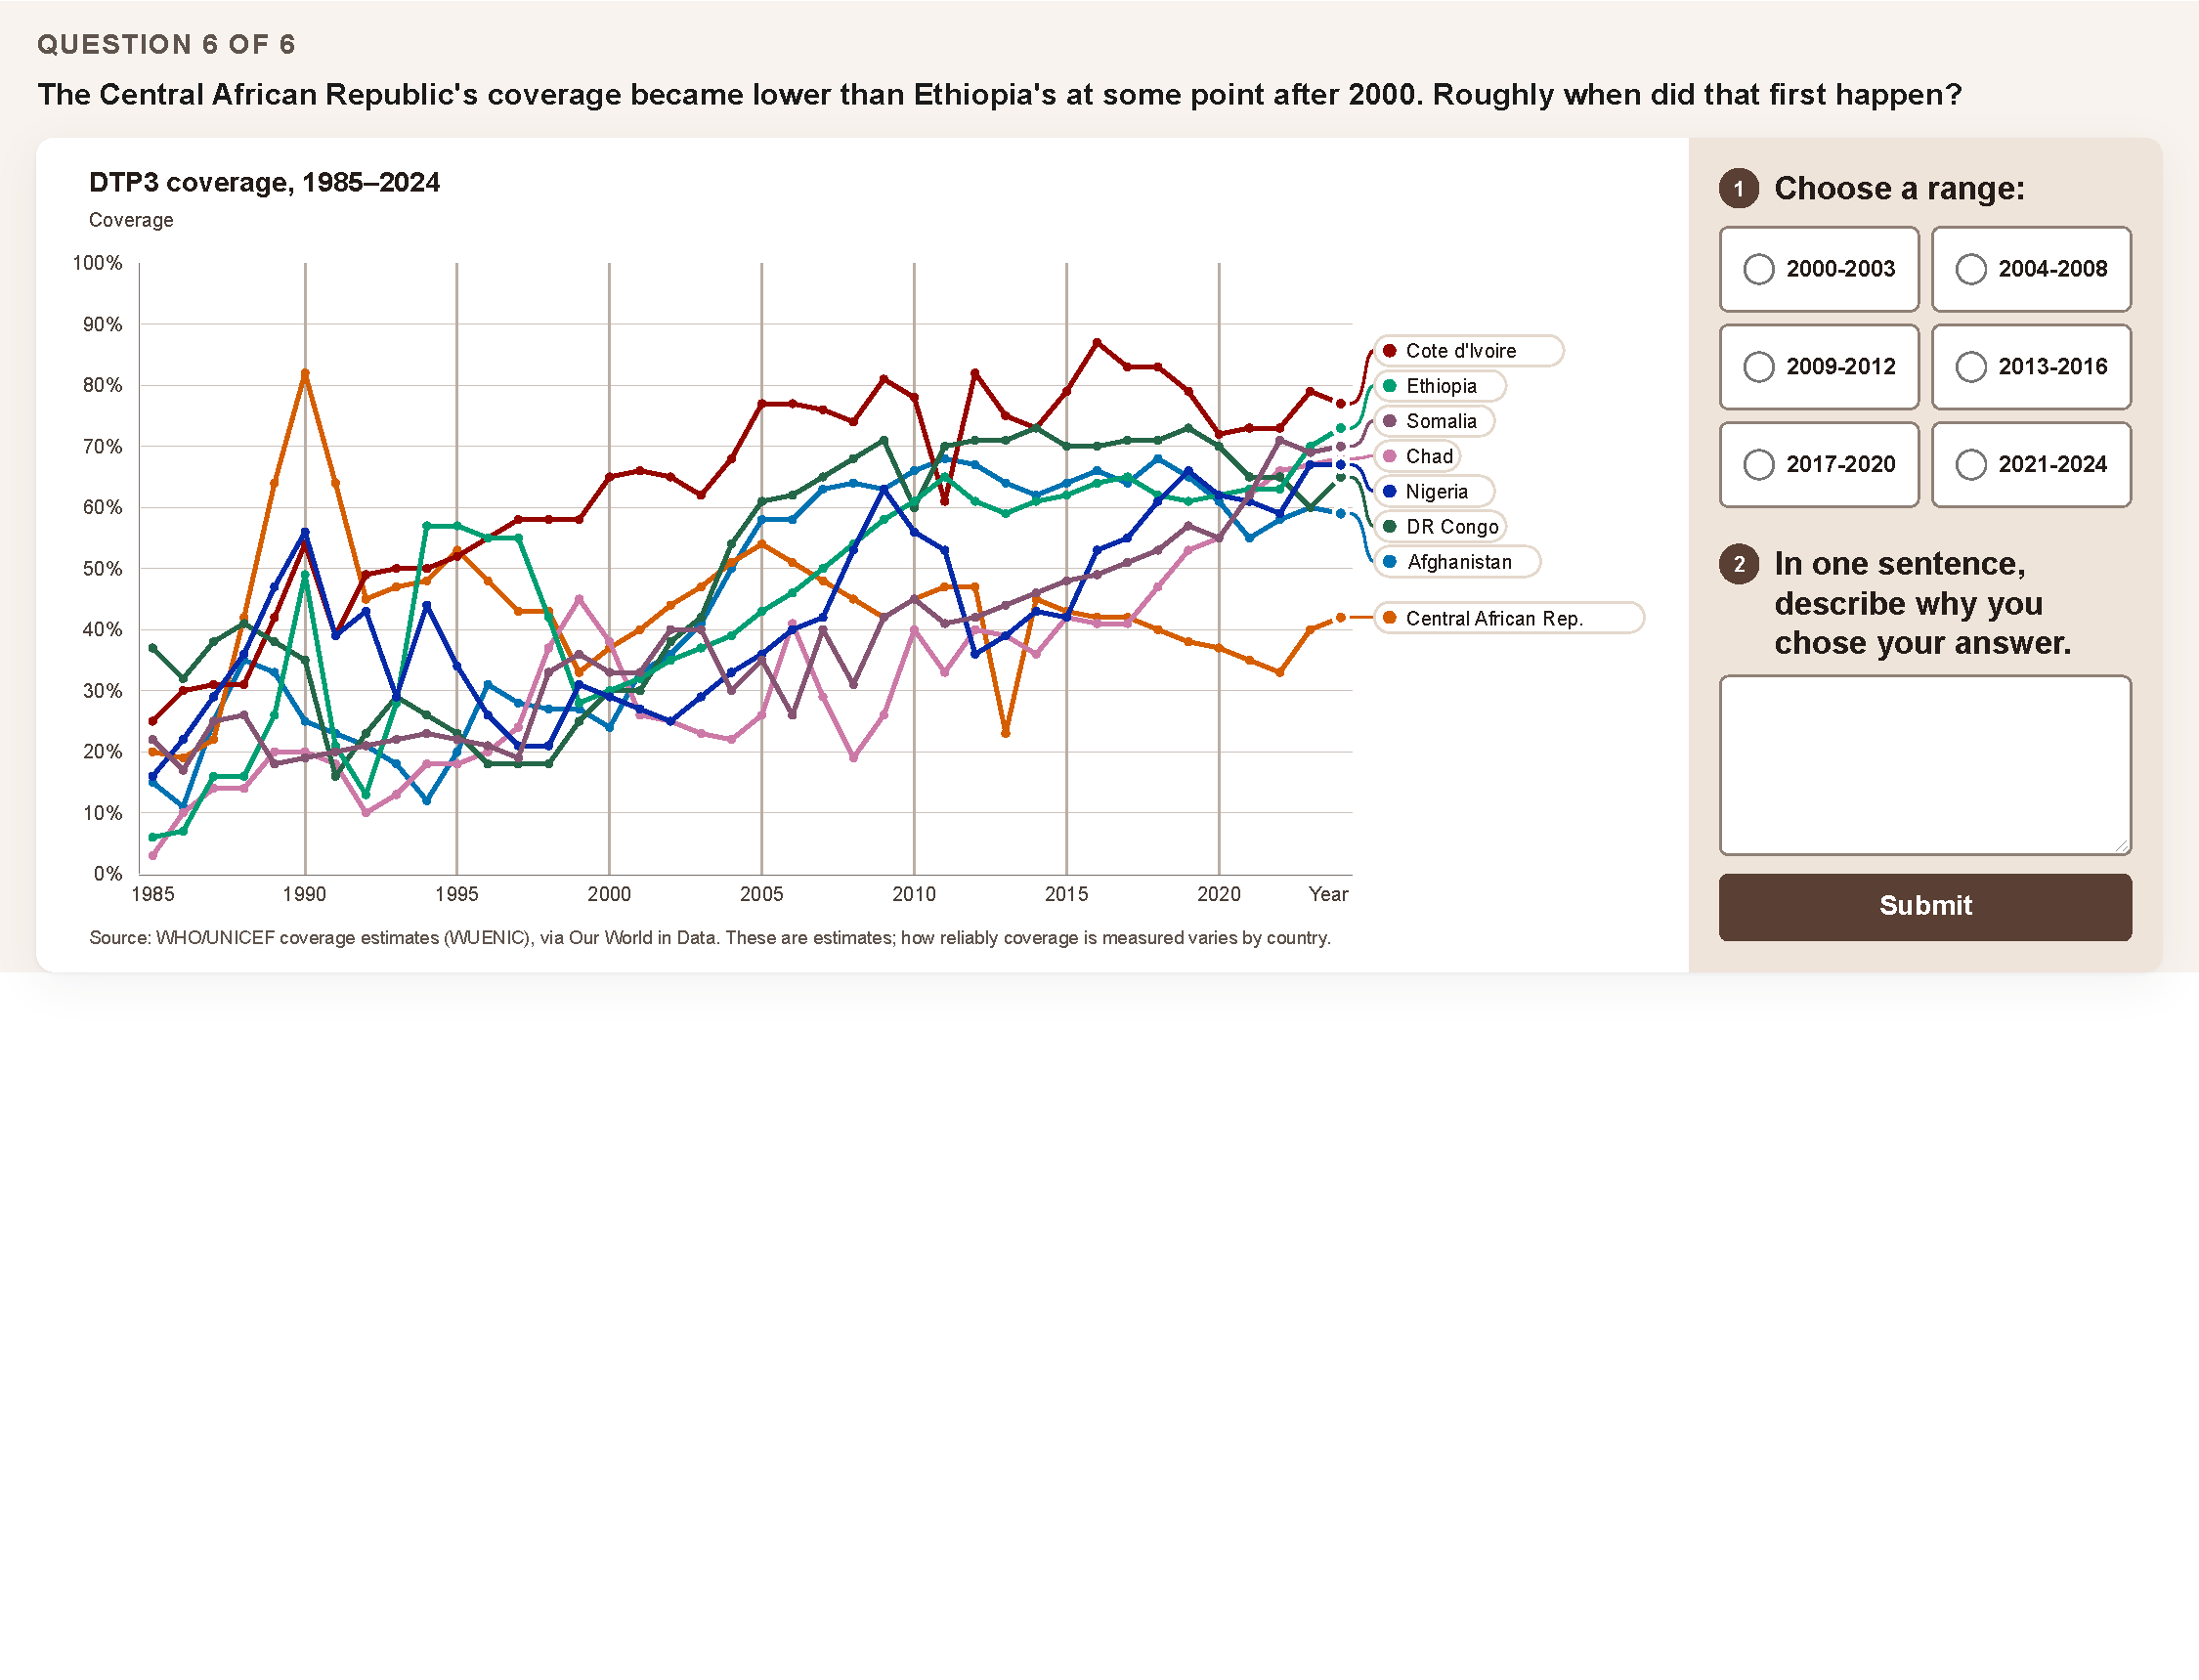
\includegraphics[page=1, trim=18bp 347.96bp 250.5bp 67.42bp, clip, width=\dimexpr\linewidth-2\fboxrule\relax]{figures/versions.pdf}}\\[6pt]
{\footnotesize\textbf{Interactive}}\\[2pt]
\fcolorbox{gridcolour}{white}{\includegraphics[page=2, trim=18bp 236.96bp 250.5bp 67.42bp, clip, width=\dimexpr\linewidth-2\fboxrule\relax]{figures/versions.pdf}}

    \caption{
        One item, A-T6, in both versions as participants saw it, cropped to the chart's card: the question above it and the answer panel to its right are not shown. The chart is the same figure in both. The static version shows it as an image that responds to nothing; the interactive version adds the controls beneath it, a tooltip on hover, and focusing a line by clicking it.
    }
    \label{fig:versions}
\end{figure}
% END CLAUDE DRAFT

% BEGIN CLAUDE DRAFT: Tasks
\subsection{Tasks}
\label{sec:tasks}

Each participant answered \stat{design/items} scored items with each version, \stat{design/totalitems} in all, after an unscored practice item. The items come in \stat{design/forms} parallel forms, A and B, with the same item types on the same chart types in the same order but different countries and years. A participant used one form with each version and never the same form twice, so no question was answered twice. Each item pairs a chart type with the control that should make it easier, after the low-level analytic tasks of Amar et al.~\cite{amar2005}:

\begin{itemize}
    \item \textbf{T1} (line chart, \stat{design/entities/T1} countries): describe how two named countries' coverage changed between \stat{design/askedfrom} and \stat{design/yearlast}, and how their trends compare.
    \item \textbf{T2} (bar chart, \stat{design/entities/T2} countries): which country had the \stat{design/T2/rank/A}-highest coverage (form B: the \stat{design/T2/rank/B}-highest).
    \item \textbf{T3} (scatter plot, \stat{design/entities/T3} countries, placed by their coverage in \stat{design/askedfrom} and \stat{design/yearlast}): which country improved the most.
    \item \textbf{T4} (heatmap, \stat{design/entities/T4} countries over \stat{design/heatmapyears} years): which country holds the single lowest cell (form B: the highest).
    \item \textbf{T5} (map, \stat{design/entities/T5} African countries): how many had coverage below \stat{design/T5/threshold}\%.
    \item \textbf{T6} (line chart, \stat{design/entities/T6} countries): roughly when one named country's coverage first passed another's after \stat{design/askedfrom}.
\end{itemize}

T2 to T6 offer \stat{design/options} options each, and T6's are year ranges. Static readers cannot read exact values, so no item asks for one, and every answer was checked against the data to survive the reading errors of a reader without hover: no answer turns on a difference of less than \stat{design/floor/position} percentage points on an axis or \stat{design/floor/colour} on a colour scale, and no scatter dot sits within \stat{design/floor/dots} points of another. Where such a control helps, it saves effort rather than making the question answerable.

T1 differs from the rest in two ways. It is the only written item, the one that asks for an interpretation of a time series rather than a value or a relation. In the interactive version it also carried \stat{design/extracontrols} controls that its question does not need, which no instruction named: a coverage range, a reordering of the country buttons, region filters, and switches for the points and name tags. They test whether more controls than a question needs make it harder. On T1, interactivity and the extra controls cannot be told apart, so any difference on T1 belongs to the overloaded interface, not to interactivity alone.
% END CLAUDE DRAFT

% BEGIN CLAUDE DRAFT: Procedure
\subsection{Procedure}
\label{sec:procedure}

Sessions ran in person on campus, and participants used their own computers. A session ran in this order: the consent form, a participant ID, instructions, the practice item, the first version's items and survey, a break, instructions for the other version, its items on the other form and its survey, questions about the participant's background, and a closing screen that asked them not to discuss the questions with anyone. Each participant's order of versions and forms came from a database sequence rather than a random draw, so the orders filled evenly: \stat{main/cells/int1-A} participants met the interactive version first on form A, \stat{main/cells/int1-B} first on form B, \stat{main/cells/int2-A} second on form A and \stat{main/cells/int2-B} second on form B.

Instructions came before both halves, so that a participant who met the interactive version second still had every control described before using it; the practice item, a line chart, taught the interface once. The instructions named every control except T1's extra ones, and the first screen asked for a full-screen window. Any question could be skipped after a confirmation. Signed consent was stored apart from the study data and could not be linked to it, and participants could withdraw their data within the period the consent form set.

The protocol had the researcher say the same few things in every session, answer any other question with ``please do whatever you would do on your own'', and record nothing but the application's own log. In practice the sessions departed from it. They were audio-recorded, and participants were often asked to think aloud; the researcher's answers to questions varied; and some debriefs disclosed answers, scores or the study's purpose while collection was still running \unverified. Table~\ref{tab:deviations} lists these and every other deviation. \todo{HSRRC's approval of the recordings: its date and how it was given.}
% END CLAUDE DRAFT

% BEGIN CLAUDE DRAFT: Deviations (table and caption, from paper/deviations.md)
\subsection{Deviations}
\label{sec:deviations}

Table~\ref{tab:deviations} lists every way the study as run departs from its pre-registration and protocol, and whether each came before or after the confirmatory tests.

\begin{table*}[t]
    \footnotesize
    \begin{tabular}{p{0.65\textwidth}p{0.17\textwidth}p{0.1\textwidth}}
        \toprule
        \textbf{Deviation} & \textbf{When} & \textbf{Tests} \\
        \midrule
        Collection closed at \stat{main/n}, one short of the target of \stat{design/targetn}. & 10 Nov. 2026 & before \\
        Participant 19 reinstated. Their interactive half was opened twice, leaving an empty session that the pre-registered rule counts as incomplete. The main analysis drops that session and re-runs every rule; the pre-registered analysis, without them, is reported beside it. & 10--11 Nov. 2026 & before \\
        One grader instead of two: an AI model drafted every code from blind sheets, and the author reviewed every one. No agreement statistic exists. The review changed \stat{review/t1/changed} of \stat{review/t1/codes} rubric codes and \stat{review/rq2/changed} of \stat{review/rq2/codes} justification codes. & 11 Nov. 2026, before any answer was read & before \\
        The uncertainty code dropped from reasoning depth. & 11 Nov. 2026, before unblinding & before \\
        The inference plan written after looks at the data: averages from part of the sample, then a poster of averages, before any test. & 3--11 Nov. 2026 & before \\
        The supervisor's answers to the plan's open questions. & \todo{date} & after \\
        Sessions audio-recorded, and participants asked informally to think aloud\textsuperscript{\dag}. & during collection & before \\
        Researcher input varied between sessions: clarifications, cues to use the controls, tools permitted\textsuperscript{\dag}. & during collection & before \\
        Answers, scores and the design disclosed in debriefs while collection was running\textsuperscript{\dag}. & during collection & before \\
        One joint session, two participants side by side on the same items\textsuperscript{\dag}. & during collection & before \\
        One item (A-T6) reworded after the first participant, naming the same crossing from the other line; its key unchanged. & 14 Oct. 2026 & before \\
        Windows smaller than the layout assumed: \stat{main/windows/compact} of \stat{main/windows/participants} were \stat{design/compactheight} pixels tall or less, so some interactive cards scrolled. & measured 11 Nov. 2026 & after \\
        The plan's equivalence test of accuracy, run with the main tests, not reported; left to future work (Section~\ref{sec:conclusion}). The plan's verdict on RQ3 does not change. & 22 Nov. 2026 & after \\
        \bottomrule
    \end{tabular}
    \caption{
        Deviations from the pre-registration and the protocol, in the order they arose. The confirmatory tests ran once, on 11 November 2026, and the last column says whether each deviation came before or after that run. \dag~Rests on a first, AI-assisted pass over the session recordings that has not yet been checked \unverified. Details are in \texttt{paper/deviations.md}.
    }
    \label{tab:deviations}
\end{table*}
% END CLAUDE DRAFT

\section{Evaluation Metrics}
\label{sec:evaluation}

% BEGIN CLAUDE DRAFT: Measures
\subsection{Measures}
\label{sec:measures}

\textbf{Accuracy (RQ1).} The proportion of the \stat{design/items} items a participant answered correctly with each version, a skipped answer scoring incorrect. T2 to T6 are scored against keys derived from the data by the rule each item states. T1 is scored against a rubric of \stat{design/t1parts} parts: (a) the first country's coverage rose; (b) the other's fell and then recovered; (c) one overtook the other, or they ended close. A description is correct when it states every part and contradicts none. How many parts it states correctly is a secondary score.

\textbf{Reasoning depth (RQ2).} Each justification of a T2 to T6 answer, and each T1 description, was coded for whether it cites values (levels, changes or years read from the chart, however approximate) and whether it compares countries (names a country other than the answer). A justification's depth is the number of these it does; a participant's depth is the mean over their T2 to T6 justifications in each version, and depth with T1 is a secondary. The coding was blind to version: the sheets held only an opaque identifier and the text, in shuffled order.

\textbf{Mental effort (RQ3).} After each version, participants rated the effort they had invested on the Paas scale~\cite{paas1992}, from \stat{design/paasmin}, ``very, very low mental effort'', to \stat{design/paaspoints}, ``very, very high mental effort''. The survey then asked \stat{design/surveyitems} statements on a \stat{design/likertpoints}-point agreement scale, among them one that also concerns effort (a7, ``Answering the questions took a lot of mental effort''), which is reported beside the Paas rating and never in its place. After the interactive version, \stat{design/controlsitems} statements asked about the controls, one of them whether the participant had hovered to see exact values; after the second version, participants said which version helped them answer more accurately and which they preferred.

\textbf{Time and the use of controls.} Time on each item came from the participant's browser clock, so that network delays and server start-up do not enter it; when a page reload reset that clock, the time was recorded as missing rather than as a wrong number. The application logged every use of a control except hovering, which it did not log.

\textbf{Exclusions,} fixed before collection. A participant without two complete halves leaves every analysis, and so does an answer given in under \stat{design/fastseconds} seconds. A time the clock could not measure, or above the \stat{design/trimpercentile}th percentile of all times, leaves only the time analysis.
% END CLAUDE DRAFT

\subsection{Analysis}
\label{sec:analysis}

% BEGIN CLAUDE DRAFT: Analysis
\textbf{Two analyses.} Participant 19's interactive half was opened twice within a second, which left an empty extra session, so the pre-registered rule for incomplete sessions, as written, removes all of this participant's answers. The main analysis drops the empty session and applies every rule unchanged ($n = \stat{main/n}$). The analysis as pre-registered ($n = \stat{pre/n}$) is reported beside it, and where a conclusion differs between the two, the paper says so.

\textbf{The main tests.} Each research question has one score per participant and version: the proportion correct over the \stat{design/items} items (RQ1), the mean depth of the T2 to T6 justifications (RQ2), and the Paas rating (RQ3). Each is tested on the participants' differences, interactive minus static, with the two-period crossover analysis of Section~\ref{sec:background}: the difference is regressed on the half in which the participant used the interactive version and on the form it showed, and the intercept estimates the effect of interactivity adjusted for both. Each estimate is reported with its 95\% confidence interval, $t$, its degrees of freedom, $p$ and $d_z$. Two checks do not assume normally distributed differences: a Wilcoxon signed-rank test for all three, and, for accuracy, which takes few values and is often equal in both versions, a permutation test that re-deals each participant's order \stat{design/permutations} times.

\textbf{Three tests.} Holm's correction holds the \stat{design/family} main tests together to a familywise error rate of $\alpha = \stat{design/alpha}$, so the smallest $p$ must clear \stat{design/holmfirst}. Only these tests may be called significant. The proposal's question, whether interactivity reduces effort rather than improving accuracy, can be answered yes only if the Paas rating falls significantly.

\textbf{Secondary outcomes} are estimated with the same model and never tested: time per item, as a ratio of geometric means; accuracy over answered items only; accuracy without the participants who had heard details of the study beforehand; T1's parts score; reasoning depth with T1; and how often justifications cited values or compared countries. Results by item and the survey are described, not tested, since no chart type carries enough items to be tested on its own.

\textbf{What this sample can detect.} With $n = \stat{main/n}$ and \stat{design/power}\% power, a main test detects an effect of $d_z = \stat{main/sensitivity/single}$ at $\alpha = \stat{design/alpha}$, and of $d_z = \stat{main/sensitivity/holm}$ at Holm's first step, so only large effects were likely to be found. A non-significant result is therefore reported as not detected, never as no effect~\cite{altman1995}.

\textbf{When the plan was written.} The measures and the exclusion rules were fixed before collection; the inference plan was not. It was drafted on 3 November 2026, after a look at the distributions and averages of the participants run by then, and written into the protocol on 11 November, after a poster of averages and before any test. The tests then ran once, that day. A plan fixed in advance is what keeps a test from being chosen for its result~\cite{cockburn2018}; this one was fixed before the tests but after those looks, and Table~\ref{tab:deviations} records it.

\textbf{Measures considered and not used.} NASA-TLX~\cite{hart1988} rates workload on several subscales, but with only two versions per participant the extra scales would have cost time without adding resolution, so the single Paas item measured effort. Eye tracking would show where participants looked, but collecting biometric data raises consent and privacy concerns beyond this study's scope. Insight-based evaluation~\cite{north2006,saraiya2006} counts the insights participants report, but a fixed rubric gives more reproducible scores. A formal think-aloud protocol~\cite{ericsson1993,carpendale2008} would show reasoning as it happens, but could not be run consistently across sessions in the time available; informal think-aloud entered the sessions anyway (Section~\ref{sec:procedure}). Agreement between two coders, measured by Cohen's $\kappa$~\cite{cohen1960}, was planned; with one grader it could not be computed.
% END CLAUDE DRAFT

\section{Results and Discussion}
\label{sec:results}

% BEGIN CLAUDE DRAFT: Results, lead-in
Every main result is given for the main analysis and, beside it, as pre-registered; no conclusion differs between the two. Tables~\ref{tab:tests} and~\ref{tab:secondary} give every estimate in full, and the text reports those the conclusions rest on.
% END CLAUDE DRAFT

\subsection{Sample and Exclusions}
\label{sec:sample}

% BEGIN CLAUDE DRAFT: Sample and exclusions
The main analysis has \stat{main/n} participants and the analysis as pre-registered \stat{pre/n}, since there the rule for incomplete sessions removes participant 19's \stat{pre/excl/incomplete_session/rows} answers (Table~\ref{tab:exclusions}). No answer fell under the \stat{design/fastseconds}-second rule, so every other answer counts toward accuracy. Times are thinner. Page reloads reset the browser's clock on \stat{main/excl/invalid_timing/rows} answers, from \stat{main/timing/invalidparticipants} participants, and the \stat{main/excl/top_one_percent/rows} longest times, all above \stat{main/timing/cutoff} seconds, were trimmed. That left \stat{main/timing/notime} participant with no usable time in one version, so the time analysis has $n = \stat{main/log_time/n}$. No session was logged through a database outage. Participants skipped \stat{main/skips/interactive/answers} answer with the interactive version and \stat{main/skips/static/answers} with the static one.
% END CLAUDE DRAFT

% BEGIN CLAUDE DRAFT: caption (the table is generated: tables/exclusions.tex)
\begin{table}[t]
    \centering
    \footnotesize
    % GENERATED by scripts/paper_figures.py. Do not edit by hand.
% The pre-registered exclusions, in the order they run, for both analyses.

\begin{tabular}{@{}>{\raggedright\arraybackslash}p{0.42\linewidth}>{\raggedright\arraybackslash}p{0.22\linewidth}rr@{}}
\toprule
Rule & Removes from & Main & Pre-reg. \\
\midrule
Did not finish both halves & Every outcome & \stat{main/excl/incomplete_session/rows} (\stat{main/excl/incomplete_session/participants}) & \stat{pre/excl/incomplete_session/rows} (\stat{pre/excl/incomplete_session/participants}) \\
Answered in under \stat{design/fastseconds}~s & Every outcome & \stat{main/excl/too_fast/rows} & \stat{pre/excl/too_fast/rows} \\
No usable time from the browser & Time only & \stat{main/excl/invalid_timing/rows} & \stat{pre/excl/invalid_timing/rows} \\
Time above the \stat{design/trimpercentile}th percentile & Time only & \stat{main/excl/top_one_percent/rows} & \stat{pre/excl/top_one_percent/rows} \\
Logged through a database outage & Time, re-run & \stat{main/excl/degraded_session/rows} (\stat{main/excl/degraded_session/sessions}) & \stat{pre/excl/degraded_session/rows} (\stat{pre/excl/degraded_session/sessions}) \\
\bottomrule
\end{tabular}

    \caption{
        The pre-registered exclusions, in the order they run: the answers each removed in the main analysis and as pre-registered, with the participants or sessions it covers in brackets. The third and fourth remove only an answer's time, and only from the time analysis. A session logged through a database outage would be kept, and the time analysis run again without it.
    }
    \label{tab:exclusions}
\end{table}
% END CLAUDE DRAFT

\subsection{Accuracy (RQ1)}
\label{sec:accuracy}

% BEGIN CLAUDE DRAFT: Accuracy
Accuracy with the interactive version differed from accuracy with the static one by \stat{main/accuracy/items/est} items of \stat{design/items} (95\% CI \stat{main/accuracy/items/ci}; Table~\ref{tab:tests}). In proportion correct the estimate is \stat{main/accuracy/est} \stat{main/accuracy/ci}, $t$(\stat{main/accuracy/df}) = \stat{main/accuracy/t}, $p$ = \stat{main/accuracy/p}, Holm $p$ = \stat{main/accuracy/holm}, $d_z$ = \stat{main/accuracy/dz}: not significant. This does not show that accuracy was unchanged (Section~\ref{sec:analysis}): the interval includes differences in either direction, most of them in the interactive version's favour.

The checks agree (Wilcoxon $p$ = \stat{main/accuracy/wilcoxon}; permutation $p$ = \stat{main/accuracy/permutation}), and the individual differences show how little room there was for one (Figure~\ref{fig:accuracy}). Of the \stat{main/n} participants, \stat{main/accuracy/diff/zero} scored the same with both versions, \stat{main/accuracy/diff/above} did better with the interactive one and \stat{main/accuracy/diff/below} with the static one; \stat{main/ceiling/static} got every item right with the static version, and \stat{main/ceiling/interactive} with the interactive one. As pre-registered, the estimate is \stat{pre/accuracy/items/est} items \stat{pre/accuracy/items/ci}, Holm $p$ = \stat{pre/accuracy/holm}, again not significant. The secondary estimates agree: \stat{main/accuracy_answered/est} over answered items only, and \stat{main/accuracy_no_heard/est} without the \stat{main/heard/yes} participant who had heard details of the study beforehand (Table~\ref{tab:secondary}).

\textbf{By item.} The items differed from one another far more than the versions did (Table~\ref{tab:items}, Figure~\ref{fig:items}). T5 was at ceiling, every answer correct with both versions, and T2 and T4 were near it, at \stat{main/item/T2/static/pct}\% and \stat{main/item/T4/static/pct}\% even with the static version. T1, the written item, was near the floor (Section~\ref{sec:overload}). The room for a difference lay mostly in T3 and T6. T6 rose from \stat{main/item/T6/static/pct}\% to \stat{main/item/T6/interactive/pct}\%, in both forms. T3 barely moved overall (\stat{main/item/T3/static/pct}\% and \stat{main/item/T3/interactive/pct}\%) and moved in opposite directions in the two forms: from \stat{main/item/T3/A/static/pct}\% to \stat{main/item/T3/A/interactive/pct}\% on form A, and from \stat{main/item/T3/B/static/pct}\% to \stat{main/item/T3/B/interactive/pct}\% on form B. With credit for the band next to the key, T6 reaches \stat{main/item/T6/static/adjacentpct}\% and \stat{main/item/T6/interactive/adjacentpct}\%: every interactive error, and some static ones, placed the crossing one band away. No answer chose 2000--2003, the band nearest the crossings before 2000 that the question set aside. Static accuracy on T2, T4 and T5 was far above what guessing among \stat{design/options} options would give, so the items' reading floors (Section~\ref{sec:tasks}) held without hover. The ceiling took power from the test, but it does not by itself explain the result. None of these differences was tested.
% END CLAUDE DRAFT

% BEGIN CLAUDE DRAFT: caption (the table is generated: tables/tests.tex)
\begin{table*}[t]
    \centering
    \footnotesize
    % GENERATED by scripts/paper_figures.py. Do not edit by hand.
% The three main tests (Holm family) and the equivalence test, both analyses.

\begin{tabular}{@{}lrlrrrrr@{}}
\toprule
Outcome & $n$ & Estimate [95\% CI] & $t$ (df) & $p$ & Holm $p$ & Wilcoxon $p$ & $d_z$ \\
\midrule
\multicolumn{8}{@{}l}{\emph{Main analysis: participant 19 reinstated}} \\
RQ1 accuracy (proportion correct) & \stat{main/accuracy/n} & \stat{main/accuracy/est} \stat{main/accuracy/ci} & \stat{main/accuracy/t} (\stat{main/accuracy/df}) & \stat{main/accuracy/p} & \stat{main/accuracy/holm} & \stat{main/accuracy/wilcoxon} & \stat{main/accuracy/dz} \\
\quad in items, of \stat{design/items} &  & \stat{main/accuracy/items/est} \stat{main/accuracy/items/ci} &  &  &  &  &  \\
\quad equivalence at $\pm$\stat{design/boundprop}: 90\% CI, TOST $p$ &  & \stat{main/tost/ci} &  & \stat{main/tost/p} & \multicolumn{3}{l}{\stat{main/tost/short}} \\
RQ2 reasoning depth (codes per justification) & \stat{main/depth/n} & \stat{main/depth/est} \stat{main/depth/ci} & \stat{main/depth/t} (\stat{main/depth/df}) & \stat{main/depth/p} & \stat{main/depth/holm} & \stat{main/depth/wilcoxon} & \stat{main/depth/dz} \\
RQ3 mental effort (Paas, \stat{design/paasmin}--\stat{design/paaspoints}) & \stat{main/paas/n} & \stat{main/paas/est} \stat{main/paas/ci} & \stat{main/paas/t} (\stat{main/paas/df}) & \stat{main/paas/p} & \stat{main/paas/holm} & \stat{main/paas/wilcoxon} & \stat{main/paas/dz} \\
\addlinespace
\multicolumn{8}{@{}l}{\emph{As pre-registered: without participant 19}} \\
RQ1 accuracy (proportion correct) & \stat{pre/accuracy/n} & \stat{pre/accuracy/est} \stat{pre/accuracy/ci} & \stat{pre/accuracy/t} (\stat{pre/accuracy/df}) & \stat{pre/accuracy/p} & \stat{pre/accuracy/holm} & \stat{pre/accuracy/wilcoxon} & \stat{pre/accuracy/dz} \\
\quad in items, of \stat{design/items} &  & \stat{pre/accuracy/items/est} \stat{pre/accuracy/items/ci} &  &  &  &  &  \\
\quad equivalence at $\pm$\stat{design/boundprop}: 90\% CI, TOST $p$ &  & \stat{pre/tost/ci} &  & \stat{pre/tost/p} & \multicolumn{3}{l}{\stat{pre/tost/short}} \\
RQ2 reasoning depth (codes per justification) & \stat{pre/depth/n} & \stat{pre/depth/est} \stat{pre/depth/ci} & \stat{pre/depth/t} (\stat{pre/depth/df}) & \stat{pre/depth/p} & \stat{pre/depth/holm} & \stat{pre/depth/wilcoxon} & \stat{pre/depth/dz} \\
RQ3 mental effort (Paas, \stat{design/paasmin}--\stat{design/paaspoints}) & \stat{pre/paas/n} & \stat{pre/paas/est} \stat{pre/paas/ci} & \stat{pre/paas/t} (\stat{pre/paas/df}) & \stat{pre/paas/p} & \stat{pre/paas/holm} & \stat{pre/paas/wilcoxon} & \stat{pre/paas/dz} \\
\bottomrule
\end{tabular}

    \caption{
        The three main tests, which Holm's correction treats as one family, in the main analysis and as pre-registered. Each estimate is interactive minus static, from the crossover analysis adjusted for half and form, with its 95\% confidence interval; accuracy is also given in items, of \stat{design/items}. Only these three tests can be called significant, at $\alpha = \stat{design/alpha}$ after Holm's correction.
    }
    \label{tab:tests}
\end{table*}
% END CLAUDE DRAFT

% BEGIN CLAUDE DRAFT: caption (the figure is generated: figures/accuracy.tex)
\begin{figure}[t]
    \centering
    % GENERATED by scripts/paper_figures.py. Do not edit by hand.
% Each participant's accuracy difference in items (main analysis), as a count per value; each analysis's estimate with its 95% CI.
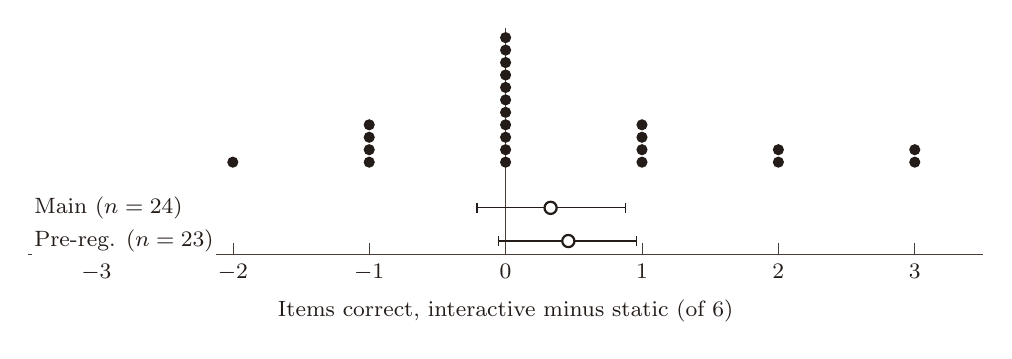
\begin{tikzpicture}
\begin{axis}[
  paper dots,
  y=4.5pt,
  xmin=-3.5, xmax=3.5,
  ymin=-6.4, ymax=11.8,
  xtick={-3,-2,-1,0,1,2,3},
  xlabel={Items correct, interactive minus static (of 6)},
]
\draw[axiscolour] (axis cs:0,-6.4) -- (axis cs:0,11.8);
\addplot[only marks, mark=*, mark size=1.8pt, inkcolour] coordinates {(-2,1) (-1,1) (-1,2) (-1,3) (-1,4) (0,1) (0,2) (0,3) (0,4) (0,5) (0,6) (0,7) (0,8) (0,9) (0,10) (0,11) (1,1) (1,2) (1,3) (1,4) (2,1) (2,2) (3,1) (3,2)};
\node[anchor=west, inner sep=1pt, xshift=1pt, fill=white, font=\footnotesize, text=inkcolour] at (axis cs:-3.5,-2.6667) {Main ($n=24$)};
\draw[inkcolour] (axis cs:-0.21,-2.6667) -- (axis cs:0.88,-2.6667);
\draw[inkcolour] (axis cs:-0.21,-3.0667) -- (axis cs:-0.21,-2.2667);
\draw[inkcolour] (axis cs:0.88,-3.0667) -- (axis cs:0.88,-2.2667);
\addplot[only marks, mark=*, mark size=2.2pt, inkcolour, mark options={fill=white, line width=0.8pt}] coordinates {(0.33,-2.6667)};
\node[anchor=west, inner sep=1pt, xshift=1pt, fill=white, font=\footnotesize, text=inkcolour] at (axis cs:-3.5,-5.3333) {Pre-reg. ($n=23$)};
\draw[inkcolour] (axis cs:-0.05,-5.3333) -- (axis cs:0.96,-5.3333);
\draw[inkcolour] (axis cs:-0.05,-5.7333) -- (axis cs:-0.05,-4.9333);
\draw[inkcolour] (axis cs:0.96,-5.7333) -- (axis cs:0.96,-4.9333);
\addplot[only marks, mark=*, mark size=2.2pt, inkcolour, mark options={fill=white, line width=0.8pt}] coordinates {(0.46,-5.3333)};
\end{axis}
\end{tikzpicture}

    \caption{
        Each participant's difference in accuracy, in items correct of \stat{design/items}, interactive minus static: one dot per participant of the main analysis. Beneath, the estimate (white dot) of the main analysis and of the pre-registered one (Pre-reg.), with its 95\% confidence interval. The estimates come from the crossover analysis, adjusted for half and form, so they need not equal the mean of the dots.
    }
    \label{fig:accuracy}
\end{figure}
% END CLAUDE DRAFT

% BEGIN CLAUDE DRAFT: caption (the table is generated: tables/items.tex)
\begin{table}[t]
    \centering
    \footnotesize
    % GENERATED by scripts/paper_figures.py. Do not edit by hand.
% Accuracy and median time by item and version, main analysis.

\begin{tabular}{@{}llrrrrr@{}}
\toprule
 &  &  & \multicolumn{2}{c}{Correct (\%)} & \multicolumn{2}{c}{Median time (s)} \\
\cmidrule(lr){4-5} \cmidrule(l){6-7}
Item & Chart & $n$ & Static & Interactive & Static & Interactive \\
\midrule
T1 & line & \stat{main/item/T1/static/n} & \stat{main/item/T1/static/pct} & \stat{main/item/T1/interactive/pct} & \stat{main/item/T1/static/seconds} & \stat{main/item/T1/interactive/seconds} \\
T2 & bar & \stat{main/item/T2/static/n} & \stat{main/item/T2/static/pct} & \stat{main/item/T2/interactive/pct} & \stat{main/item/T2/static/seconds} & \stat{main/item/T2/interactive/seconds} \\
T3 & scatter & \stat{main/item/T3/static/n} & \stat{main/item/T3/static/pct} & \stat{main/item/T3/interactive/pct} & \stat{main/item/T3/static/seconds} & \stat{main/item/T3/interactive/seconds} \\
T4 & heatmap & \stat{main/item/T4/static/n} & \stat{main/item/T4/static/pct} & \stat{main/item/T4/interactive/pct} & \stat{main/item/T4/static/seconds} & \stat{main/item/T4/interactive/seconds} \\
T5 & map & \stat{main/item/T5/static/n} & \stat{main/item/T5/static/pct} & \stat{main/item/T5/interactive/pct} & \stat{main/item/T5/static/seconds} & \stat{main/item/T5/interactive/seconds} \\
T6 & line & \stat{main/item/T6/static/n} & \stat{main/item/T6/static/pct} & \stat{main/item/T6/interactive/pct} & \stat{main/item/T6/static/seconds} & \stat{main/item/T6/interactive/seconds} \\
\bottomrule
\end{tabular}

    \caption{
        Accuracy and median time by item and version, main analysis; Appendix~\ref{app:preregistered} gives the table as pre-registered. Each row pools forms A and B. No item was tested on its own. Median times are over every answer whose time was recorded, the longest ones trimmed from the time analysis among them.
    }
    \label{tab:items}
\end{table}
% END CLAUDE DRAFT

% BEGIN CLAUDE DRAFT: caption (the figure is generated: figures/items.tex)
\begin{figure}[t]
    \centering
    % GENERATED by scripts/paper_figures.py. Do not edit by hand.
% Accuracy by item and version (main analysis).

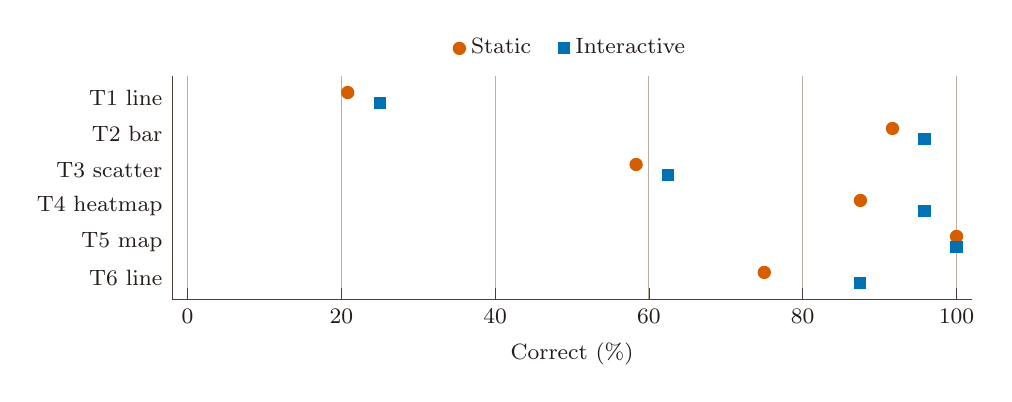
\begin{tikzpicture}
\begin{axis}[
  paper,
  width=\linewidth-56pt,
  y=13pt,
  xmin=-2, xmax=102, xtick={0,20,...,100},
  ymin=0.4, ymax=6.6,
  ytick={1,...,6},
  yticklabels={{T6 line},{T5 map},{T4 heatmap},{T3 scatter},{T2 bar},{T1 line}},
  ytick style={draw=none},
  xmajorgrids, grid style={gridcolour},
  xlabel={Correct (\%)},
  legend style={at={(0.5,1.03)}, anchor=south, /tikz/every even column/.append style={column sep=8pt}}, legend columns=2,
]
\addplot[only marks, mark=*, mark size=2.2pt, staticcolour] coordinates {(20.8333,6.15) (91.6667,5.15) (58.3333,4.15) (87.5,3.15) (100,2.15) (75,1.15)};
\addlegendentry{Static}
\addplot[only marks, mark=square*, mark size=2pt, interactivecolour] coordinates {(25,5.85) (95.8333,4.85) (62.5,3.85) (95.8333,2.85) (100,1.85) (87.5,0.85)};
\addlegendentry{Interactive}
\end{axis}
\end{tikzpicture}

    \caption{
        Percentage correct on each item, static (circles) and interactive (squares), main analysis, drawn slightly apart so that equal values stay visible. Descriptive: no item was tested on its own.
    }
    \label{fig:items}
\end{figure}
% END CLAUDE DRAFT

\subsection{Reasoning Depth (RQ2)}
\label{sec:depth}

% BEGIN CLAUDE DRAFT: Reasoning depth
A difference in reasoning depth was not detected. Justifications written with the interactive version carried \stat{main/depth/est} codes more, on average, than those written with the static one (95\% CI \stat{main/depth/ci}; Holm $p$ = \stat{main/depth/holm}), on a scale with a maximum of \stat{design/depthmax}, where the means were \stat{main/depth/static/mean} and \stat{main/depth/interactive/mean}. As pre-registered, the estimate is \stat{pre/depth/est} \stat{pre/depth/ci}. Counting T1's descriptions changes little: \stat{main/depth_with_t1/est} \stat{main/depth_with_t1/ci}. The two codes moved in opposite directions, which their sum hides. The share of justifications citing values changed by \stat{main/cites_values/est}, from \stat{main/cites_values/static/pct}\% to \stat{main/cites_values/interactive/pct}\%, consistent with the exact values that hover offers; the share comparing countries changed by \stat{main/compares_series/est}, from \stat{main/compares_series/static/pct}\% to \stat{main/compares_series/interactive/pct}\%. Both intervals include zero in the main analysis. As pre-registered, the interval for citing values, \stat{pre/cites_values/ci}, does not, but it is a secondary estimate, untested, and it changes with one participant (Table~\ref{tab:secondary}).
% END CLAUDE DRAFT

\subsection{Mental Effort (RQ3)}
\label{sec:effort}

% BEGIN CLAUDE DRAFT: Mental effort
A difference in rated mental effort was not detected (Figure~\ref{fig:effort}). The Paas rating changed by \stat{main/paas/est} points with the interactive version (95\% CI \stat{main/paas/ci}), $t$(\stat{main/paas/df}) = \stat{main/paas/t}, $p$ = \stat{main/paas/p}, Holm $p$ = \stat{main/paas/holm}, $d_z$ = \stat{main/paas/dz}; as pre-registered, by \stat{pre/paas/est} \stat{pre/paas/ci}, Holm $p$ = \stat{pre/paas/holm}. The interval runs from a drop of more than a point to a small rise, so the data cannot say whether rated effort changed. The estimated effect is about half the smallest one this design could reliably detect at Holm's first step ($d_z$ = \stat{main/sensitivity/holm}), so its failure to reach significance is not evidence that effort was unchanged.

The survey's own effort statement, a7, moved further. Mean agreement that answering took a lot of mental effort was \stat{main/survey/a7/static/mean} after the static version and \stat{main/survey/a7/interactive/mean} after the interactive one, on a scale to \stat{design/likertpoints}. It is reported beside the Paas rating, never in its place, and only described; Section~\ref{sec:survey} sets the two side by side.

The proposal's question is therefore left open. Its ``rather than'' could be answered yes only if rated effort fell significantly, and it did not, so the plan's verdict is ``\stat{main/rq3/verdict}''. As the plan prescribes for this case, the effect on accuracy is unclear: a difference was not detected, which is not evidence that there was none.
% END CLAUDE DRAFT

% BEGIN CLAUDE DRAFT: caption (the figure is generated: figures/effort.tex)
\begin{figure}[t]
    \centering
    % GENERATED by scripts/paper_figures.py. Do not edit by hand.
% Each participant's change in Paas and in a7 (main analysis), as a count per value; Paas with each analysis's estimate and 95% CI. a7 is descriptive: no interval.
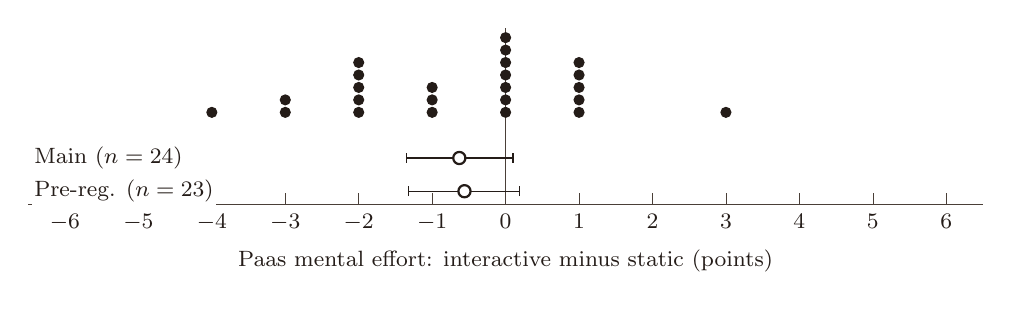
\begin{tikzpicture}
\begin{axis}[
  paper dots,
  y=4.5pt,
  xmin=-6.5, xmax=6.5,
  ymin=-6.4, ymax=7.8,
  xtick={-6,-5,-4,-3,-2,-1,0,1,2,3,4,5,6},
  xlabel={Paas mental effort: interactive minus static (points)},
]
\draw[axiscolour] (axis cs:0,-6.4) -- (axis cs:0,7.8);
\addplot[only marks, mark=*, mark size=1.8pt, inkcolour] coordinates {(-4,1) (-3,1) (-3,2) (-2,1) (-2,2) (-2,3) (-2,4) (-2,5) (-1,1) (-1,2) (-1,3) (0,1) (0,2) (0,3) (0,4) (0,5) (0,6) (0,7) (1,1) (1,2) (1,3) (1,4) (1,5) (3,1)};
\node[anchor=west, inner sep=1pt, xshift=1pt, fill=white, font=\footnotesize, text=inkcolour] at (axis cs:-6.5,-2.6667) {Main ($n=24$)};
\draw[inkcolour] (axis cs:-1.35,-2.6667) -- (axis cs:0.1,-2.6667);
\draw[inkcolour] (axis cs:-1.35,-3.0667) -- (axis cs:-1.35,-2.2667);
\draw[inkcolour] (axis cs:0.1,-3.0667) -- (axis cs:0.1,-2.2667);
\addplot[only marks, mark=*, mark size=2.2pt, inkcolour, mark options={fill=white, line width=0.8pt}] coordinates {(-0.63,-2.6667)};
\node[anchor=west, inner sep=1pt, xshift=1pt, fill=white, font=\footnotesize, text=inkcolour] at (axis cs:-6.5,-5.3333) {Pre-reg. ($n=23$)};
\draw[inkcolour] (axis cs:-1.32,-5.3333) -- (axis cs:0.19,-5.3333);
\draw[inkcolour] (axis cs:-1.32,-5.7333) -- (axis cs:-1.32,-4.9333);
\draw[inkcolour] (axis cs:0.19,-5.7333) -- (axis cs:0.19,-4.9333);
\addplot[only marks, mark=*, mark size=2.2pt, inkcolour, mark options={fill=white, line width=0.8pt}] coordinates {(-0.56,-5.3333)};
\end{axis}
\end{tikzpicture}

\medskip

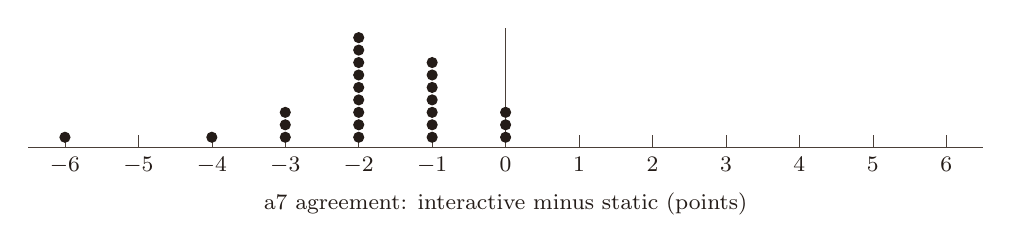
\begin{tikzpicture}
\begin{axis}[
  paper dots,
  y=4.5pt,
  xmin=-6.5, xmax=6.5,
  ymin=0.2, ymax=9.8,
  xtick={-6,-5,-4,-3,-2,-1,0,1,2,3,4,5,6},
  xlabel={a7 agreement: interactive minus static (points)},
]
\draw[axiscolour] (axis cs:0,0.2) -- (axis cs:0,9.8);
\addplot[only marks, mark=*, mark size=1.8pt, inkcolour] coordinates {(-6,1) (-4,1) (-3,1) (-3,2) (-3,3) (-2,1) (-2,2) (-2,3) (-2,4) (-2,5) (-2,6) (-2,7) (-2,8) (-2,9) (-1,1) (-1,2) (-1,3) (-1,4) (-1,5) (-1,6) (-1,7) (0,1) (0,2) (0,3)};
\end{axis}
\end{tikzpicture}

    \caption{
        Each participant's change in rated mental effort, interactive minus static, one dot per participant of the main analysis. Top: the Paas scale, from \stat{design/paasmin} to \stat{design/paaspoints}, with the estimate and 95\% confidence interval of the main analysis and of the pre-registered one (Pre-reg.). Bottom: a7, agreement from \stat{design/likertmin} to \stat{design/likertpoints} that answering took a lot of mental effort, which is descriptive and has no interval. The two scales differ, so their spreads cannot be compared point for point.
    }
    \label{fig:effort}
\end{figure}
% END CLAUDE DRAFT

\subsection{Time on Task (Exploratory)}
\label{sec:time}

% BEGIN CLAUDE DRAFT: Time on task
Time on task is exploratory: a secondary outcome, estimated and not tested. It is also the clearest effect in the data (Figure~\ref{fig:time}). An item took \stat{main/log_time/est} times as long with the interactive version (95\% CI \stat{main/log_time/ci}), about \stat{main/log_time/pct}\% longer and, within the interval, between \stat{main/log_time/lowpct}\% and \stat{main/log_time/highpct}\% longer; the estimate is the same as pre-registered (Table~\ref{tab:secondary}). The geometric mean per item was \stat{main/time/static/seconds} seconds with the static version and \stat{main/time/interactive/seconds} with the interactive one, and \stat{main/log_time/diff/above} of the \stat{main/log_time/diff/n} participants with usable times were slower with the controls. The interval excludes no difference, but making time a main test now would choose the test by its result, so it stays an estimate. Time also absorbs whatever else happened in a session: many participants were asked to think aloud, and talking lengthens tasks~\cite{fox2011} (Section~\ref{sec:limitations}).
% END CLAUDE DRAFT

% BEGIN CLAUDE DRAFT: caption (the table is generated: tables/secondary.tex)
\begin{table*}[t]
    \centering
    \footnotesize
    % GENERATED by scripts/paper_figures.py. Do not edit by hand.
% The secondary outcomes, both analyses: estimates, not tests of the hypotheses.

\begin{tabular}{@{}lrlrrlr@{}}
\toprule
 & \multicolumn{3}{c}{Main} & \multicolumn{3}{c}{As pre-registered} \\
\cmidrule(lr){2-4} \cmidrule(l){5-7}
Outcome & $n$ & Estimate [95\% CI] & $p$ & $n$ & Estimate [95\% CI] & $p$ \\
\midrule
Time per item (ratio, interactive to static) & \stat{main/log_time/n} & $\times$\stat{main/log_time/est} \stat{main/log_time/ci} & \stat{main/log_time/p} & \stat{pre/log_time/n} & $\times$\stat{pre/log_time/est} \stat{pre/log_time/ci} & \stat{pre/log_time/p} \\
Accuracy, answered items only & \stat{main/accuracy_answered/n} & \stat{main/accuracy_answered/est} \stat{main/accuracy_answered/ci} & \stat{main/accuracy_answered/p} & \stat{pre/accuracy_answered/n} & \stat{pre/accuracy_answered/est} \stat{pre/accuracy_answered/ci} & \stat{pre/accuracy_answered/p} \\
Accuracy, without those who had heard details & \stat{main/accuracy_no_heard/n} & \stat{main/accuracy_no_heard/est} \stat{main/accuracy_no_heard/ci} & \stat{main/accuracy_no_heard/p} & \stat{pre/accuracy_no_heard/n} & \stat{pre/accuracy_no_heard/est} \stat{pre/accuracy_no_heard/ci} & \stat{pre/accuracy_no_heard/p} \\
T1 parts score (of \stat{design/t1parts}) & \stat{main/t1_parts/n} & \stat{main/t1_parts/est} \stat{main/t1_parts/ci} & \stat{main/t1_parts/p} & \stat{pre/t1_parts/n} & \stat{pre/t1_parts/est} \stat{pre/t1_parts/ci} & \stat{pre/t1_parts/p} \\
Reasoning depth, with T1 & \stat{main/depth_with_t1/n} & \stat{main/depth_with_t1/est} \stat{main/depth_with_t1/ci} & \stat{main/depth_with_t1/p} & \stat{pre/depth_with_t1/n} & \stat{pre/depth_with_t1/est} \stat{pre/depth_with_t1/ci} & \stat{pre/depth_with_t1/p} \\
Justifications citing values (share) & \stat{main/cites_values/n} & \stat{main/cites_values/est} \stat{main/cites_values/ci} & \stat{main/cites_values/p} & \stat{pre/cites_values/n} & \stat{pre/cites_values/est} \stat{pre/cites_values/ci} & \stat{pre/cites_values/p} \\
Justifications comparing countries (share) & \stat{main/compares_series/n} & \stat{main/compares_series/est} \stat{main/compares_series/ci} & \stat{main/compares_series/p} & \stat{pre/compares_series/n} & \stat{pre/compares_series/est} \stat{pre/compares_series/ci} & \stat{pre/compares_series/p} \\
\bottomrule
\end{tabular}

    \caption{
        The pre-registered secondary outcomes, interactive minus static (time as a ratio), each with its 95\% confidence interval, in the main analysis and as pre-registered. They are estimates, not tests of the hypotheses: none is corrected for multiplicity, and none can be called significant, whatever its $p$.
    }
    \label{tab:secondary}
\end{table*}
% END CLAUDE DRAFT

% BEGIN CLAUDE DRAFT: caption (the figure is generated: figures/time.tex)
\begin{figure}[t]
    \centering
    % GENERATED by scripts/paper_figures.py. Do not edit by hand.
% Exploratory. Each participant's time ratio, interactive to static (main analysis), sorted by value; each analysis's estimate and 95% CI.

\begin{tikzpicture}
\begin{axis}[
  paper dots,
  xmode=log,
  y=3.2pt,
  xmin=0.5065, xmax=2.7005,
  ymin=-9, ymax=23.8,
  xtick={0.67,1,1.5,2},
  xticklabels={0.67,1,1.5,2},
  minor xtick={},
  xlabel={Time per item, interactive $\div$ static (log scale)},
]
\draw[axiscolour] (axis cs:1,-9) -- (axis cs:1,23.8);
\addplot[only marks, mark=*, mark size=1.5pt, inkcolour] coordinates {(0.5572,1) (0.6305,2) (0.7057,3) (0.8235,4) (0.8954,5) (0.9267,6) (1.0219,7) (1.0891,8) (1.0989,9) (1.1412,10) (1.1656,11) (1.2525,12) (1.3025,13) (1.3173,14) (1.3344,15) (1.3373,16) (1.4089,17) (1.5084,18) (1.5224,19) (1.6474,20) (1.7447,21) (1.982,22) (2.455,23)};
\node[anchor=west, inner sep=1pt, xshift=1pt, fill=white, font=\footnotesize, text=inkcolour] at (axis cs:0.5065,-3.75) {Main ($n=23$)};
\draw[inkcolour] (axis cs:1.05,-3.75) -- (axis cs:1.3,-3.75);
\draw[inkcolour] (axis cs:1.05,-4.3125) -- (axis cs:1.05,-3.1875);
\draw[inkcolour] (axis cs:1.3,-4.3125) -- (axis cs:1.3,-3.1875);
\addplot[only marks, mark=*, mark size=2.2pt, inkcolour, mark options={fill=white, line width=0.8pt}] coordinates {(1.17,-3.75)};
\node[anchor=west, inner sep=1pt, xshift=1pt, fill=white, font=\footnotesize, text=inkcolour] at (axis cs:0.5065,-7.5) {Pre-reg. ($n=22$)};
\draw[inkcolour] (axis cs:1.05,-7.5) -- (axis cs:1.3,-7.5);
\draw[inkcolour] (axis cs:1.05,-8.0625) -- (axis cs:1.05,-6.9375);
\draw[inkcolour] (axis cs:1.3,-8.0625) -- (axis cs:1.3,-6.9375);
\addplot[only marks, mark=*, mark size=2.2pt, inkcolour, mark options={fill=white, line width=0.8pt}] coordinates {(1.17,-7.5)};
\end{axis}
\end{tikzpicture}

    \caption{
        Exploratory. Each participant's time per item with the interactive version divided by their time with the static one (a ratio of geometric means), on a log scale, sorted: one dot per participant of the main analysis with a usable time in both versions. Beneath, the estimate and 95\% confidence interval of the main analysis and of the pre-registered one (Pre-reg.). Above 1, the interactive version took longer.
    }
    \label{fig:time}
\end{figure}
% END CLAUDE DRAFT

\subsection{The Overloaded Item, the Controls and Hover}
\label{sec:overload}

% BEGIN CLAUDE DRAFT: The overloaded item, the controls and hover
\textbf{T1, the overloaded item.} T1 was hard with either version: only \stat{main/item/T1/static/pct}\% of descriptions were correct with the static version, and \stat{main/item/T1/interactive/pct}\% with the interactive one, which carried \stat{design/extracontrols} controls the question did not need. Over the times the time analysis keeps, T1's median time was \stat{main/t1/static/seconds} and \stat{main/t1/interactive/seconds} seconds; Table~\ref{tab:items}'s medians, which keep every recorded time, differ for that reason. Of the \stat{main/t1extra/n} participants, \stat{main/t1extra/users} used at least one of the extra controls: the region filters (\stat{main/t1extra/regions/users} participants), the coverage range (\stat{main/t1extra/coverage/users}), the order of the country buttons (\stat{main/t1extra/order/users}) and the switches for points and name tags (\stat{main/t1extra/display/users}). The parts score, a secondary, changed by \stat{main/t1_parts/est} \stat{main/t1_parts/ci} of \stat{design/t1parts} parts. On T1 the overload and interactivity cannot be told apart, so any of these differences belongs to the overloaded interface, never to interactivity alone.

\textbf{The controls and hover.} The logs show which controls participants found with the interactive version. The bar chart's sort was used on T2 by \stat{main/controls/T2/sort} of \stat{main/controls/T2/n} participants, and the heatmap's row sort on T4 by \stat{main/controls/T4/sort}. The key's colours, built into the chart rather than placed beneath it, were used far less: on T3 by \stat{main/controls/T3/key}, on T4 by \stat{main/controls/T4/key} and on T5 by \stat{main/controls/T5/key}. On the line charts, the country buttons were used on T6 by \stat{main/controls/T6/chips}, and the chart was narrowed to start in 2000 or later, with the Years slider or by zooming, on T1 by \stat{main/from2000/T1/either} and on T6 by \stat{main/from2000/T6/either}. Hover was not logged. Participants' own rating of whether they hovered to see exact values (b4) averaged \stat{main/survey/b4/interactive/mean} of \stat{design/likertpoints}, so most say they did, though on no particular item. A logged control is evidence of use, but the absence of one is not evidence of no interaction: a correct interactive answer on T3, T4 or T6 may rest on a hover the logs cannot see.
% END CLAUDE DRAFT

\subsection{The Survey, Preference and the Exploratory Descriptives}
\label{sec:survey}

% BEGIN CLAUDE DRAFT: The survey, preference and the exploratory descriptives
\textbf{The survey.} Participants rated the interactive version far more favourably (Table~\ref{tab:survey}). Agreement that it was easy to compare countries (a6) rose from \stat{main/survey/a6/static/mean} to \stat{main/survey/a6/interactive/mean}, and a2 to a5, on understanding the charts, finding information, reading values and seeing changes, rose by similar margins. Confidence (a1) rose from \stat{main/survey/a1/static/mean} to \stat{main/survey/a1/interactive/mean}, and frustration (a8) fell from \stat{main/survey/a8/static/mean} to \stat{main/survey/a8/interactive/mean}. After both halves, \stat{main/c1/controls} of \stat{main/n} participants said the charts with controls helped them answer more accurately, and \stat{main/c2/controls} preferred them. These numbers are descriptive, and their context weighs on them. Many participants were the researcher's friends or co-workers \unverified, the study's purpose was described aloud before the tasks in some sessions \unverified, and everyone knew the researcher had built the system. Participants favour an artifact they believe the researcher made~\cite{dell2012}, and satisfaction tracks performance only weakly~\cite{hornbaek2007}. The preference is therefore a finding about how the versions felt, not evidence of how well they worked.

\textbf{Exploratory descriptives.} These were listed and defined after the tests and before any was computed; none is a test. Of T1's rubric parts, (c), that one country overtook the other or that they ended close, was the lowest of the three with both versions, credited in \stat{main/t1rubric/all/static/c}\% of static descriptions and \stat{main/t1rubric/all/interactive/c}\% of interactive ones. Paas and a7 agreed only weakly (Spearman's $\rho$ = \stat{main/paasa7/rho/all}): a7 fell for \stat{main/paasa7/a7lower} of \stat{main/paasa7/participants} participants and Paas for \stat{main/paasa7/paaslower}, and the ratings of \stat{main/paasa7/reversed} participants looked as if the Paas scale had been read backwards, though no one was excluded for it. The a7 rating fell further when the interactive version came second (a change of \stat{main/order/second/a7/diff}) than when it came first (\stat{main/order/first/a7/diff}), while the Paas rating changed by about the same either way (\stat{main/order/second/paas/diff} and \stat{main/order/first/paas/diff}). Of the \stat{main/c1acc/controls/n} who said the controls helped their accuracy, \stat{main/c1acc/controls/higher} scored higher with them, \stat{main/c1acc/controls/equal} the same and \stat{main/c1acc/controls/lower} lower. Finally, the author's review of the AI-drafted grading codes changed \stat{review/t1/changed} of \stat{review/t1/codes} rubric codes, \stat{review/t1/changed/interactive} of them on interactive answers, each crediting a part the draft had missed and making a description correct; it changed \stat{review/rq2/changed} of \stat{review/rq2/codes} justification codes. The grading rules gained \stat{rules/all} rules during grading. The review started from the draft, so these counts are not an agreement statistic.
% END CLAUDE DRAFT

% BEGIN CLAUDE DRAFT: caption (the table is generated: tables/survey.tex)
\begin{table*}[t]
    \centering
    \footnotesize
    % GENERATED by scripts/paper_figures.py. Do not edit by hand.
% The survey, main analysis: mean (SD) of each statement, and c1 and c2's counts.

\begin{tabular}{@{}lp{0.52\textwidth}rll@{}}
\toprule
 & Statement & $n$ & Static & Interactive \\
\midrule
\multicolumn{5}{@{}l}{\emph{After each version: agreement, \stat{design/likertmin}--\stat{design/likertpoints}}} \\
a1 & I am confident that my answers in this part were correct. & \stat{main/survey/a1/static/n} & \stat{main/survey/a1/static/mean} (\stat{main/survey/a1/static/sd}) & \stat{main/survey/a1/interactive/mean} (\stat{main/survey/a1/interactive/sd}) \\
a2 & The charts were easy to understand. & \stat{main/survey/a2/static/n} & \stat{main/survey/a2/static/mean} (\stat{main/survey/a2/static/sd}) & \stat{main/survey/a2/interactive/mean} (\stat{main/survey/a2/interactive/sd}) \\
a3 & I could quickly find the information I needed. & \stat{main/survey/a3/static/n} & \stat{main/survey/a3/static/mean} (\stat{main/survey/a3/static/sd}) & \stat{main/survey/a3/interactive/mean} (\stat{main/survey/a3/interactive/sd}) \\
a4 & I could read values from the charts as precisely as the questions required. & \stat{main/survey/a4/static/n} & \stat{main/survey/a4/static/mean} (\stat{main/survey/a4/static/sd}) & \stat{main/survey/a4/interactive/mean} (\stat{main/survey/a4/interactive/sd}) \\
a5 & It was easy to see where coverage increased or decreased. & \stat{main/survey/a5/static/n} & \stat{main/survey/a5/static/mean} (\stat{main/survey/a5/static/sd}) & \stat{main/survey/a5/interactive/mean} (\stat{main/survey/a5/interactive/sd}) \\
a6 & It was easy to compare countries with each other. & \stat{main/survey/a6/static/n} & \stat{main/survey/a6/static/mean} (\stat{main/survey/a6/static/sd}) & \stat{main/survey/a6/interactive/mean} (\stat{main/survey/a6/interactive/sd}) \\
a7 & Answering the questions took a lot of mental effort. & \stat{main/survey/a7/static/n} & \stat{main/survey/a7/static/mean} (\stat{main/survey/a7/static/sd}) & \stat{main/survey/a7/interactive/mean} (\stat{main/survey/a7/interactive/sd}) \\
a8 & I felt frustrated while answering the questions. & \stat{main/survey/a8/static/n} & \stat{main/survey/a8/static/mean} (\stat{main/survey/a8/static/sd}) & \stat{main/survey/a8/interactive/mean} (\stat{main/survey/a8/interactive/sd}) \\
a9 & I felt rushed while answering the questions. & \stat{main/survey/a9/static/n} & \stat{main/survey/a9/static/mean} (\stat{main/survey/a9/static/sd}) & \stat{main/survey/a9/interactive/mean} (\stat{main/survey/a9/interactive/sd}) \\
\addlinespace
\multicolumn{5}{@{}l}{\emph{After the interactive version only, \stat{design/likertmin}--\stat{design/likertpoints}}} \\
b1 & I could figure out how to use the chart controls without instructions. & \stat{main/survey/b1/interactive/n} & -- & \stat{main/survey/b1/interactive/mean} (\stat{main/survey/b1/interactive/sd}) \\
b2 & The chart controls helped me answer the questions. & \stat{main/survey/b2/interactive/n} & -- & \stat{main/survey/b2/interactive/mean} (\stat{main/survey/b2/interactive/sd}) \\
b3 & The chart controls were easy to use. & \stat{main/survey/b3/interactive/n} & -- & \stat{main/survey/b3/interactive/mean} (\stat{main/survey/b3/interactive/sd}) \\
b4 & I hovered over the charts to see exact values. & \stat{main/survey/b4/interactive/n} & -- & \stat{main/survey/b4/interactive/mean} (\stat{main/survey/b4/interactive/sd}) \\
\addlinespace
\multicolumn{5}{@{}l}{\emph{After the second version: participants choosing each answer}} \\
c1 & Which charts helped you answer more accurately? & & \multicolumn{2}{l}{} \\
 & \multicolumn{4}{l}{\quad With controls \stat{main/c1/controls}; Without controls \stat{main/c1/nocontrols}; No difference \stat{main/c1/nodifference}; Skipped \stat{main/c1/skipped}} \\
c2 & Which charts did you prefer using? & & \multicolumn{2}{l}{} \\
 & \multicolumn{4}{l}{\quad With controls \stat{main/c2/controls}; Without controls \stat{main/c2/nocontrols}; No difference \stat{main/c2/nodifference}; Skipped \stat{main/c2/skipped}} \\
\bottomrule
\end{tabular}

    \caption{
        The survey, main analysis; Appendix~\ref{app:preregistered} gives it as pre-registered. Mean agreement (SD) with each statement after each version, the statements about the controls after the interactive version only, and how many participants chose each answer to the two questions asked after the second version. Descriptive.
    }
    \label{tab:survey}
\end{table*}
% END CLAUDE DRAFT

\subsection{Qualitative Observations}
\label{sec:qualitative}

% BEGIN CLAUDE DRAFT: Qualitative observations
The sessions were audio-recorded and transcribed with Whisper~\cite{radford2023}, and names and places were removed from the transcripts. An AI model then made a first pass of thematic coding~\cite{braun2006} over the transcripts and the researcher's session notes. It was a single coder, not blind to version, and its excerpts have not yet been checked against the recordings \unverified. The talk is informal comment, not a think-aloud protocol~\cite{ericsson1993}, and how much each participant said varied widely, so silence is not an absence of reasoning. Each theme below therefore comes with an example and never with a count of the participants who raised it~\cite{mcdonald2019}.

\textbf{Getting rid of lines.} To participants, interactivity mostly meant filtering: hiding countries to cut through the crowded line charts, which they described as overwhelming in the static version. \todo{exemplar from paper/private/quotes.md, theme 1.} This fits the preference results, but it is not by itself evidence that filtering improved accuracy.

\textbf{The key read as a reference, not a control.} Several participants took the controls beneath the chart to be its only interactive part and never discovered that a colour in the key could be clicked, which matches how rarely the logs show the key in use. \todo{exemplar, theme 2.} Some found it by chance or from experience with other tools; the instructions described it, but few participants read them in full.

\textbf{Exact values change the method.} On the scatter plot (T3), participants with hover read values from the tooltip and subtracted them, where without it they judged distances by eye. \todo{exemplar, theme 3.} This is the clearest qualitative case that interactivity changed how a question was answered, even though T3's accuracy barely differed.

\textbf{Item wording behind errors.} Many errors in the talk came from the questions rather than the version: what ``the single lowest'' cell meant on T4, and colours whose meaning changed from one chart to the next. \todo{exemplar, theme 4.} These bear on the items' validity more than on interactivity.
% END CLAUDE DRAFT

\subsection{Discussion}
\label{sec:discussion}

% BEGIN CLAUDE DRAFT: Discussion
Interactivity clearly changed how the charts felt; whether it changed how well they were read, this study could not show. A difference in accuracy was not detected, and its interval leans toward the interactive version but includes no difference and a small disadvantage. Whether interactivity lowered the effort participants invested is unclear, since the Paas estimate pointed down but its interval included no change. The interactive version took longer, an exploratory estimate, and participants preferred it, in a sample inclined to prefer it.

The mini-project~\cite{rebollar2026mini}, with \stat{mini/n} participants split between the versions, found comparable accuracy, longer times with interaction (\stat{mini/time/interactive} against \stat{mini/time/static}) and lower reported load: agreement that the dashboard felt overwhelming fell by \stat{mini/overwhelming} points on a \stat{mini/likertpoints}-point scale. With a within-subjects design, parallel forms and times from the browser, accuracy and time behaved here as they did there. Lower load did not survive as a tested result, although the survey's own effort statement, a7, fell from \stat{main/survey/a7/static/mean} to \stat{main/survey/a7/interactive/mean}. One result reversed. The mini-project's static users were slightly more confident (\stat{mini/confidence/static} against \stat{mini/confidence/interactive}); here confidence rose with the controls, from \stat{main/survey/a1/static/mean} to \stat{main/survey/a1/interactive/mean}, while a difference in accuracy was not detected. Confidence outrunning accuracy is the outcome the proposal worried about. These data are consistent with it, though no test addressed it.

Several things may have kept a difference in accuracy from appearing, and none explains the result alone. The first is the design itself: every item passed a rule that kept its answer readable without hover, so the controls could make an answerable question easier but never make an unanswerable one answerable. The second is the items: T5 was at ceiling and T2 and T4 near it, so a difference could show easily only on T3 and T6. The third is discovery. Controls beneath the chart were widely used, but the clickable key, built into the chart, was used on T3 by \stat{main/controls/T3/key} of \stat{main/controls/T3/n} participants, consistent with the key being read as a reference rather than a control (Section~\ref{sec:qualitative}) and with what studies of how people discover interactivity lead one to expect~\cite{blascheck2019}. The fourth is hover, which was not logged, so on T3 and T6, where it might have mattered most, its use is unknown. Finally, interaction has costs of its own, in deciding what to do and in doing it~\cite{lam2008}. The extra time may have bought confidence rather than accuracy, much as an animated display once bought enjoyment rather than accuracy~\cite{robertson2008}.

For designers, three cautions follow, within this sample and this platform. A control needs a visible signifier to be used: those under the chart were found, and the one inside it mostly was not. Interactivity should not be expected to save time; here it cost time. And a reader's preference or confidence is weak evidence of how accurately a chart is read~\cite{hornbaek2007}, so a dashboard is better judged by what its readers get right. T1 suggests a fourth, weaker one. Its unneeded controls drew a minority of participants and did not visibly harm accuracy, but T1 sat near the floor with both versions, so it says little about the cost of an overloaded interface.
% END CLAUDE DRAFT

\subsection{Limitations}
\label{sec:limitations}

% BEGIN CLAUDE DRAFT: Limitations
\begin{itemize}
    \item \textbf{The sample} is small: \stat{main/n} participants, one short of the target, from one community, mostly undergraduates and many of them the researcher's friends or co-workers \unverified. The results describe this sample, not the wider and more varied population that uses dashboards; HCI studies lean heavily on samples like it~\cite{linxen2021}.
    \item \textbf{One platform.} Every chart was built with one library, so nothing here shows whether the findings hold on another.
    \item \textbf{One grader.} An AI model drafted every grading code and the author reviewed each one. The author knew the hypotheses, and without a second coder there is no measure of agreement. The sheets were blind to version, but a description that quotes exact values can hint at the interactive one.
    \item \textbf{The plan's timing.} The inference plan was written after looks at the data (Section~\ref{sec:analysis}), so the tests are less firmly confirmatory than a plan fixed before collection would have made them~\cite{cockburn2018}.
    \item \textbf{The items.} T5 was at ceiling and T2 and T4 near it, leaving little room for a difference, while T1 sat near the floor and confounds the overload with interactivity. The forms are not equivalent: T2 and T4 ask different questions in each form, T1's falling line falls much further on form A than on form B, and T6 asks about a line becoming lower on one form and higher on the other.
    \item \textbf{Hover.} Hover was not logged, so its use is known only from a self-report, and the year-over-year change in the tooltip cannot be separated from interactivity as a whole.
    \item \textbf{Windows.} Despite the request for a full-screen window, \stat{main/windows/compact} of \stat{main/windows/participants} windows were \stat{design/compactheight} pixels tall or less, so some interactive cards ran past the bottom of the screen where the static ones did not.
    \item \textbf{The protocol as run} differed from the plan (Table~\ref{tab:deviations}) \unverified. Many participants were asked to think aloud, which lengthens tasks~\cite{fox2011}; the researcher's clarifications and cues to the controls varied; some debriefs disclosed answers or the design while collection was running, so later participants may have heard them; and two participants took part side by side. Only \stat{main/heard/yes} participant reported having heard details beforehand, and setting that participant aside changed little (Section~\ref{sec:accuracy}), but the question catches only what participants report. No one was asked about colour vision.
    \item \textbf{The qualitative material} is a single AI-assisted pass, not yet checked against the recordings.
\end{itemize}
% END CLAUDE DRAFT

\section{Ethical Considerations}
\label{sec:ethics}

% BEGIN CLAUDE DRAFT: Ethical considerations
Visualizations shape how data inform decisions, and those who design and study them share responsibility for what readers come away believing~\cite{correll2019}. This study's charts showed childhood vaccination coverage, a domain where misreading a chart can feed decisions and arguments about public health. The ethics paper that preceded this one~\cite{rebollar2026ethics} set out the concerns; this section reports how the study met them and where it fell short.

\textbf{Who took part, and whose readings count.} The sample is small, young, mostly undergraduate and drawn largely from the researcher's own circle, as samples in HCI research often are~\cite{linxen2021,caine2016}. It leaves out the older, less formally educated and non-native-English readers who also use public dashboards, and the results say nothing about them. Scoring raises a quieter bias, because a rubric decides whose interpretation counts as correct~\cite{quadri2024}. T1's rubric credits three features of a pattern and, by rule, judges the pattern rather than the precision of its values, so a reader without exact values is not penalised for lacking them. A description built on context the rubric did not anticipate, such as a war or vaccine hesitancy, could still earn nothing for it.

\textbf{The researcher as builder.} The researcher built the system, recruited the participants and ran every session, and many participants knew the researcher personally. Participants tend to favour what they believe the researcher made~\cite{dell2012}, so the survey and preference results are reported as how the versions felt, and the tests rest on answers that could be checked against the data.

\textbf{Unequal data.} The WHO/UNICEF estimates combine countries' administrative reports with household surveys~\cite{burton2009}, and countries with weaker statistical systems are measured less reliably. Every chart's source line says that the values are estimates whose reliability varies by country. The items also drew heavily on low-coverage countries in Africa and Asia, because that is where the differences a reading task needs are found. Shown without context to readers far from those places, such charts risk a deficit framing of the countries they show. No item asks why coverage is low, and the paper draws no conclusion about any country.

\textbf{Accessibility.} The palette meets the contrast floors of WCAG 2.1~\cite{w3c2018wcag21} and keeps every pair of series colours apart under simulated colour blindness, and every control works from the keyboard except hovering and clicking a line. The study did not ask about colour vision, however, and made no provision for screen readers. Accessible dashboards have to be designed with blind and low-vision users from the start~\cite{srinivasan2023,costanzachock2020}. This study could not do that, so its results describe sighted users only.

\textbf{Consent, privacy and AI tools.} Consent was signed in the application and stored apart from the study data, without a participant identifier, so the two cannot be linked, and participants could withdraw their data within the period the consent form set. The sessions were audio-recorded, which the approved protocol said would not happen. \todo{HSRRC's approval of the recordings: its date and how it was given.} AI tools handled participant text in two places: grading, on sheets that carried an opaque identifier and the text alone, and the first pass over the session transcripts. \todo{Eduardo: say whether the AI saw the transcripts only after names and places were removed.} Neither approved form mentions AI tools; both restrict identifying data, and the grading sheets carried none. Participants' words appear in this paper only as short excerpts, never beside a background that could identify them, and the free text of the closing questions is never quoted.

\textbf{Where the data are.} \todo{what the paper says about where the data can be found: the rubric asks for the raw data in the repository, and the IRB forms keep it out.}
% END CLAUDE DRAFT

\section{Conclusion}
\label{sec:conclusion}

% BEGIN CLAUDE DRAFT: Conclusion
This study asked whether interactivity helps people interpret charts of a time series or only makes interpretation feel easier. Given two versions of the same charts that differed only in whether they responded, \stat{main/n} participants showed no detectable difference in accuracy between them (\stat{main/accuracy/items/est} items of \stat{design/items}, 95\% CI \stat{main/accuracy/items/ci}). Whether interactivity lowered the effort they invested remains open. The tested measure did not detect a change, while the survey's effort statement and participants' preferences favoured the controls strongly, and the interactive version took longer. The proposal's expectation, that interactivity reduces perceived load rather than improving accuracy, is therefore neither confirmed nor refuted: its half about effort did not reach the bar the plan set, and a difference in accuracy that was not detected is not evidence that there was none.

A next study should change what this one could not. It should log hover; give controls built into a chart a visible signifier; set items away from the ceiling; grade with a second, independent coder; fix the analysis plan before any data are seen; recruit beyond one campus and one circle of acquaintance; and repeat the comparison on a second platform. It should also test accuracy for equivalence against a bound fixed before collection~\cite{schuirmann1987,lakens2017}: such a test can show that a difference is smaller than the bound, where a test of difference, as reported here, can say only that none was detected. What this study already offers is a way to make the two versions identical by construction, so that whatever difference such a study finds can be laid at interactivity's door.
% END CLAUDE DRAFT

% BEGIN CLAUDE DRAFT: Use of AI tools (factual; for Eduardo to edit)
\section*{Use of AI Tools}

Claude, Anthropic's AI model, was used through Claude Code to write and test the study's software and analysis scripts, under the constraints the repository records. \todo{Eduardo: confirm this scope, and name the models if you want them named.} Claude (Claude Opus 5.5) drafted every grading code, the T1 rubric's and the justifications', from blind sheets that carried an opaque identifier and the text alone; the author reviewed every code, and the author's decision is final. The review changed \stat{review/t1/changed} of \stat{review/t1/codes} rubric codes and \stat{review/rq2/changed} of \stat{review/rq2/codes} justification codes. The session recordings were transcribed with OpenAI's Whisper (large-v3-turbo)~\cite{radford2023}, and Claude made a first pass of qualitative coding over the de-identified transcripts and the researcher's notes, which has not yet been checked. \todo{Eduardo: whether Whisper ran on your own computer or through a service, and what Claude saw before de-identification.} Claude Code also drafted the text of this paper: every section from the abstract to the conclusion, the deviations table, the captions, the appendices and this statement, each draft marked in its source for the author to rewrite. It found ten of the references and checked every reference added after the proposal against its registry record, and it wrote the scripts that generate every number, table and figure in the paper from the study's output and the application's code. \todo{Eduardo: once the drafts are rewritten, confirm or revise: ``The questions, the analysis plan, the interpretation and the conclusions are the author's.''}
% END CLAUDE DRAFT

\printbibliography

\appendix

\clearpage

\onecolumn

% BEGIN CLAUDE DRAFT: Appendix A
\section{Replication Instructions}
\label{app:replication}

The code is public at
\begin{center}
\url{https://github.com/EduardoRebollar/Interactivity-and-Interpretability-in-Data-Visualization-Dashboards}
\end{center}
It needs Python \stat{software/python} or later and uv (\url{https://docs.astral.sh/uv/}), which installs the exact versions recorded in \path{uv.lock}: among them Dash \stat{software/dash}, Plotly \stat{software/plotly}, pandas \stat{software/pandas}, pyarrow \stat{software/pyarrow}, psycopg \stat{software/psycopg}, pytest \stat{software/pytest} and Ruff \stat{software/ruff}. NumPy and SciPy are locked to a version for each Python release.

\paragraph{The study application.} From the repository's root:
\begin{lstlisting}[language=bash]
uv sync                                       # install the locked environment
uv run python scripts/download_data.py        # fetch the coverage data from Our World in Data
uv run python -m src.data                     # clean it into the complete grid
uv run python scripts/export_deploy_data.py   # write data/deploy/coverage.csv (also committed)
uv run python -m src.app                      # the study at http://127.0.0.1:8050
uv run pytest                                 # the test suite
\end{lstlisting}
Run locally, without a database, the application logs to files under \path{data/study_logs/} and serves \url{http://127.0.0.1:8050/preview}, which shows any item of either form in either version and records nothing. Which version a session gets follows from the participant ID, so entering different IDs reaches every order.

\paragraph{The analysis.} The study's own data are not in the repository (Ethical Considerations). \todo{Eduardo: what the paper says about access to the data.} With a database of study events, or a CSV exported from it, the pipeline runs in this order:
\begin{lstlisting}[language=bash]
uv run python scripts/score_study.py                        # score; mark the exclusions
uv run python scripts/code_justifications.py rubric-sheets  # blind sheets for T1 ...
uv run python scripts/code_justifications.py sheets         # ... and for the justifications
#   grade both sheets by docs/grading-rules.md
uv run python scripts/code_justifications.py rubric         # T1's verdicts
uv run python scripts/code_justifications.py depth          # reasoning depth
uv run python scripts/score_study.py                        # score again, with T1 coded
uv run python notebooks/significance.py                     # the confirmatory tests: once only
uv run python scripts/paper_descriptives.py                 # the exploratory descriptives
uv run python scripts/paper_numbers.py                      # paper/numbers.tex
uv run python scripts/paper_figures.py                      # paper/tables/ and paper/figures/
\end{lstlisting}
The confirmatory script ran once on this study's data, on 11 November 2026, and is not to be run on them again; \texttt{notebooks/significance.py --simulate} shows its output on made-up data. Each later step checks itself against that run and refuses to write if it disagrees. Figure~\ref{fig:versions} needs no study data, only Chrome or Edge: \texttt{scripts/paper\_figures.py --versions-only} draws it from the application's own screen code.

\paragraph{The paper.} \path{paper/main.tex} builds with \texttt{latexmk -pdf main} from \path{paper/}, or on Overleaf, using the template's \path{oxycomps.sty}, biblatex with Biber, and pgfplots for the figures.
% END CLAUDE DRAFT

% BEGIN CLAUDE DRAFT: Appendix B
\section{Code Architecture Overview}
\label{app:architecture}

The repository has four parts: the study application, which participants used; the offline analysis, which never ships with it; the scripts that run each step; and this paper. Data move through them in one direction:

\begin{enumerate}
    \item \textbf{Data.} \path{scripts/download_data.py} fetches the WHO/UNICEF estimates from Our World in Data. \path{src/data.py} cleans them into a complete grid of entity, year and vaccine, in which a value that was never reported stays missing, and \path{scripts/export_deploy_data.py} writes the committed \path{data/deploy/coverage.csv}.
    \item \textbf{The application} (\path{src/}). \path{runtime_data.py} reads that file with the standard library alone, so the deployed bundle carries no pandas. \path{figures.py} has one builder per chart type. No builder knows the version: the one switch between static and interactive is \texttt{graph\_config(interactive)}, which sets whether the browser draws the figure as an inert image, and a test checks that both versions produce identical figures for every item. \path{layout.py} draws the screens and the controls under each chart, \path{flow.py} is the session's sequence of stages, and \path{tasks.py} holds the items without their answers, since it is sent to the browser. \path{app.py} holds the callbacks, times each item in the browser, and guards Submit against double clicks. \path{logging.py} writes every event to Postgres, retrying through outages and keeping a copy in the browser until the database answers.
    \item \textbf{Scoring} (\path{analysis/}, never deployed). \path{keys.py} derives each answer from the data by the rule the item states, checks it against the protocol, and refuses an item whose answer a reader without hover could misread. \path{reshape.py} turns events into one row per answer, per half and per participant. \path{exclusions.py} applies the pre-registered rules, marking rows rather than dropping them, and \path{coding.py} writes and reads the blind coding sheets.
    \item \textbf{Inference and the paper.} \path{notebooks/significance.py} holds the confirmatory plan and ran once. \path{scripts/paper_descriptives.py} computes the exploratory descriptives, never a test. \path{scripts/paper_numbers.py} writes every number in this paper into \path{paper/numbers.tex}, which the paper reads through \texttt{\textbackslash stat}, and \path{scripts/paper_figures.py} writes its tables, which cite those numbers, and its figures, drawn by pgfplots from the same sources.
\end{enumerate}

\paragraph{Extending it.} A new item starts in \path{docs/study-design.md}, then \path{src/tasks.py}; \path{analysis/keys.py} derives its answer and refuses it if it fails the acceptance rule. A new chart type is one more builder in \path{src/figures.py}, and the test of identical figures covers it at once. A new control needs its event in \path{src/logging.py} and a column in \path{analysis/reshape.py}, since the logs are the study's data. \path{CLAUDE.md} records the project's constraints, and \path{docs/visual-spec.md} its visual decisions.
% END CLAUDE DRAFT

% BEGIN CLAUDE DRAFT: Appendix C
\section{Descriptive Tables as Pre-registered}
\label{app:preregistered}

Tables~\ref{tab:items-pre} and~\ref{tab:survey-pre} repeat Tables~\ref{tab:items} and~\ref{tab:survey} for the pre-registered analysis, without participant 19 ($n = \stat{pre/n}$).

\begin{table}[ht]
    \centering
    \footnotesize
    % GENERATED by scripts/paper_figures.py. Do not edit by hand.
% Accuracy and median time by item and version, as pre-registered.

\begin{tabular}{@{}llrrrrr@{}}
\toprule
 &  &  & \multicolumn{2}{c}{Correct (\%)} & \multicolumn{2}{c}{Median time (s)} \\
\cmidrule(lr){4-5} \cmidrule(l){6-7}
Item & Chart & $n$ & Static & Interactive & Static & Interactive \\
\midrule
T1 & line & \stat{pre/item/T1/static/n} & \stat{pre/item/T1/static/pct} & \stat{pre/item/T1/interactive/pct} & \stat{pre/item/T1/static/seconds} & \stat{pre/item/T1/interactive/seconds} \\
T2 & bar & \stat{pre/item/T2/static/n} & \stat{pre/item/T2/static/pct} & \stat{pre/item/T2/interactive/pct} & \stat{pre/item/T2/static/seconds} & \stat{pre/item/T2/interactive/seconds} \\
T3 & scatter & \stat{pre/item/T3/static/n} & \stat{pre/item/T3/static/pct} & \stat{pre/item/T3/interactive/pct} & \stat{pre/item/T3/static/seconds} & \stat{pre/item/T3/interactive/seconds} \\
T4 & heatmap & \stat{pre/item/T4/static/n} & \stat{pre/item/T4/static/pct} & \stat{pre/item/T4/interactive/pct} & \stat{pre/item/T4/static/seconds} & \stat{pre/item/T4/interactive/seconds} \\
T5 & map & \stat{pre/item/T5/static/n} & \stat{pre/item/T5/static/pct} & \stat{pre/item/T5/interactive/pct} & \stat{pre/item/T5/static/seconds} & \stat{pre/item/T5/interactive/seconds} \\
T6 & line & \stat{pre/item/T6/static/n} & \stat{pre/item/T6/static/pct} & \stat{pre/item/T6/interactive/pct} & \stat{pre/item/T6/static/seconds} & \stat{pre/item/T6/interactive/seconds} \\
\bottomrule
\end{tabular}

    \caption{
        Accuracy and median time by item and version, as pre-registered. Each row pools forms A and B, and no item was tested on its own.
    }
    \label{tab:items-pre}
\end{table}

\begin{table}[ht]
    \centering
    \footnotesize
    % GENERATED by scripts/paper_figures.py. Do not edit by hand.
% The survey, as pre-registered: mean (SD) of each statement, and c1 and c2's counts.

\begin{tabular}{@{}lp{0.52\textwidth}rll@{}}
\toprule
 & Statement & $n$ & Static & Interactive \\
\midrule
\multicolumn{5}{@{}l}{\emph{After each version: agreement, \stat{design/likertmin}--\stat{design/likertpoints}}} \\
a1 & I am confident that my answers in this part were correct. & \stat{pre/survey/a1/static/n} & \stat{pre/survey/a1/static/mean} (\stat{pre/survey/a1/static/sd}) & \stat{pre/survey/a1/interactive/mean} (\stat{pre/survey/a1/interactive/sd}) \\
a2 & The charts were easy to understand. & \stat{pre/survey/a2/static/n} & \stat{pre/survey/a2/static/mean} (\stat{pre/survey/a2/static/sd}) & \stat{pre/survey/a2/interactive/mean} (\stat{pre/survey/a2/interactive/sd}) \\
a3 & I could quickly find the information I needed. & \stat{pre/survey/a3/static/n} & \stat{pre/survey/a3/static/mean} (\stat{pre/survey/a3/static/sd}) & \stat{pre/survey/a3/interactive/mean} (\stat{pre/survey/a3/interactive/sd}) \\
a4 & I could read values from the charts as precisely as the questions required. & \stat{pre/survey/a4/static/n} & \stat{pre/survey/a4/static/mean} (\stat{pre/survey/a4/static/sd}) & \stat{pre/survey/a4/interactive/mean} (\stat{pre/survey/a4/interactive/sd}) \\
a5 & It was easy to see where coverage increased or decreased. & \stat{pre/survey/a5/static/n} & \stat{pre/survey/a5/static/mean} (\stat{pre/survey/a5/static/sd}) & \stat{pre/survey/a5/interactive/mean} (\stat{pre/survey/a5/interactive/sd}) \\
a6 & It was easy to compare countries with each other. & \stat{pre/survey/a6/static/n} & \stat{pre/survey/a6/static/mean} (\stat{pre/survey/a6/static/sd}) & \stat{pre/survey/a6/interactive/mean} (\stat{pre/survey/a6/interactive/sd}) \\
a7 & Answering the questions took a lot of mental effort. & \stat{pre/survey/a7/static/n} & \stat{pre/survey/a7/static/mean} (\stat{pre/survey/a7/static/sd}) & \stat{pre/survey/a7/interactive/mean} (\stat{pre/survey/a7/interactive/sd}) \\
a8 & I felt frustrated while answering the questions. & \stat{pre/survey/a8/static/n} & \stat{pre/survey/a8/static/mean} (\stat{pre/survey/a8/static/sd}) & \stat{pre/survey/a8/interactive/mean} (\stat{pre/survey/a8/interactive/sd}) \\
a9 & I felt rushed while answering the questions. & \stat{pre/survey/a9/static/n} & \stat{pre/survey/a9/static/mean} (\stat{pre/survey/a9/static/sd}) & \stat{pre/survey/a9/interactive/mean} (\stat{pre/survey/a9/interactive/sd}) \\
\addlinespace
\multicolumn{5}{@{}l}{\emph{After the interactive version only, \stat{design/likertmin}--\stat{design/likertpoints}}} \\
b1 & I could figure out how to use the chart controls without instructions. & \stat{pre/survey/b1/interactive/n} & -- & \stat{pre/survey/b1/interactive/mean} (\stat{pre/survey/b1/interactive/sd}) \\
b2 & The chart controls helped me answer the questions. & \stat{pre/survey/b2/interactive/n} & -- & \stat{pre/survey/b2/interactive/mean} (\stat{pre/survey/b2/interactive/sd}) \\
b3 & The chart controls were easy to use. & \stat{pre/survey/b3/interactive/n} & -- & \stat{pre/survey/b3/interactive/mean} (\stat{pre/survey/b3/interactive/sd}) \\
b4 & I hovered over the charts to see exact values. & \stat{pre/survey/b4/interactive/n} & -- & \stat{pre/survey/b4/interactive/mean} (\stat{pre/survey/b4/interactive/sd}) \\
\addlinespace
\multicolumn{5}{@{}l}{\emph{After the second version: participants choosing each answer}} \\
c1 & Which charts helped you answer more accurately? & & \multicolumn{2}{l}{} \\
 & \multicolumn{4}{l}{\quad With controls \stat{pre/c1/controls}; Without controls \stat{pre/c1/nocontrols}; No difference \stat{pre/c1/nodifference}; Skipped \stat{pre/c1/skipped}} \\
c2 & Which charts did you prefer using? & & \multicolumn{2}{l}{} \\
 & \multicolumn{4}{l}{\quad With controls \stat{pre/c2/controls}; Without controls \stat{pre/c2/nocontrols}; No difference \stat{pre/c2/nodifference}; Skipped \stat{pre/c2/skipped}} \\
\bottomrule
\end{tabular}

    \caption{
        The survey, as pre-registered. Descriptive.
    }
    \label{tab:survey-pre}
\end{table}
% END CLAUDE DRAFT

\end{document}
